\documentclass[UTF8,AutoFakeBold,AutoFakeSlant,zihao=-4,oneside,openany]{ctexbook}
% UTF8,AutoFakeBold,AutoFakeSlant,zihao=-4,oneside,openany ctexbook
% \usepackage{xeCJK}
% \usepackage{titletoc}
% \usepackage{fontspec} % unicode,但不能用暂时
% \usepackage{newunicodechar} % update unicode
\usepackage{stmaryrd} % $\lightning$
% \usepackage{setspace}
% \usepackage{graphicx} % 可以生成镜像文字
% \usepackage{fancyhdr}
% \usepackage{pdfpages} % 插入pdf页
% \usepackage{booktabs}
% \usepackage{multirow}
% \usepackage{caption}
\usepackage{tikz} % 画图
% \usepackage{etoolbox}
% \usepackage{xcolor}
% \usepackage{array}
\usepackage{amsmath} % 基本数学符号
\usepackage{amssymb} % 基本数学符号
\usepackage{mathrsfs} % \mathfrak{}
\usepackage{float} % 取消figure置顶:[H]
% \usepackage{enumerate} % 自定义列举标号样式:[(i).]
\usepackage[shortlabels]{enumitem} % enumerate自定义起始编号:[start = 42]
% \usepackage{dutchcal} % 小写花体,但大写cal也会变
\usepackage{cite} % 引用
\usepackage{color} % 搞颜色
\usepackage{mathtools} % 左上下标:\prescript{}{}{}
% \usepackage{booktabs} % 修改表格线段的粗细
% \usepackage{datetime} % 显示时间:\xxivtime \, \today
% \usepackage{scrtime} % 显示时间:\thistime \, \today
\usepackage{hyperref} % 超链接,目录默认
\usepackage{anyfontsize} % 允许任意字体大小
% \usepackage{lmodern} % 允许任意字体大小,不如anyfontsize
\usepackage{blindtext} % 允许隐藏文本
\usepackage{ifthen} % \ifthenelse 判断结构
\usepackage{eso-pic} % 在指定位置加入图片指令
\usepackage{amsxtra} % sp stuff
% \usepackage{esint} % 更多积分号:\fint
% \usepackage{stix} % \intbar,库报错
% \usepackage{MnSymbol} % \storkedint,库报错
% \usepackage{geometry} % 纸张
\usepackage{verbatim} % 多行注释:\begin{comment},库报错
% \usepackage{undertilde} % 下方波浪号:\utilde{}
\usepackage{accents}

% 纸张
\begin{comment}
\geometry{
  a4paper,
  total={170mm,257mm},
  left=20mm,
  top=20mm,
  }
\end{comment}

% 每页添加回到目录的链接
\newboolean{linktoc}
\setboolean{linktoc}{true} % true: 显示连接,false: 不显示链接

\newcommand\AtPageUpperRight[1]{\AtPageUpperLeft{%
 \put(\LenToUnit{\paperwidth},\LenToUnit{-0.3\paperheight}){#1}%
 }}%
\begin{comment}
\newcommand\AtPageLowerRight[1]{\AtPageLowerLeft{%
 \put(\LenToUnit{\paperwidth},\LenToUnit{0.3\paperheight}){#1}%
 }}%
\end{comment}

\ifthenelse{\boolean{linktoc}}%
{%
\AddToShipoutPictureBG{%
   \AtPageUpperRight{\put(-140,216){\hyperref[toc]{Go to TOC}}}
   % \AtPageLowerRight{\put(-70,0){\hyperref[toc]{Go to TOC}}}
    }%
}%
{}%

\newtheorem{sol}{Solution}
\newtheorem{rmk}{Rmk}
\newtheorem{df}{Def}
\newtheorem{ppt}{Property}
\newtheorem{prop}{Prop}
\newtheorem{lem}{Lemma}
\newtheorem{thm}{Thm}
\newtheorem{thk}{Thinking}
\newtheorem{conc}{Conculsion}
\newtheorem{pf}{Proof}
\newtheorem{eg}{Example}
\newtheorem{coro}{Corollary}

\newcommand \dbar {\hspace{0.4em} \bar{} \hspace{-0.4em} d} % 定义符号:dbar

% \newcommand*{\intbar}{\mathop{\ooalign{$\int$\cr$-$}}} % 定义符号:intbar,不好用

\setlength{\parindent}{0pt} % 取消首行缩进

\setcounter{tocdepth}{4} % 设置目录显示的章节深度
\setcounter{secnumdepth}{3} % 设置章节的编号深度

\begin{document}

\begin{Large}
  \textsc{Notes}
\end{Large}

\begin{comment}

To Do:

Ruler:规定书写规则和语法表(先规定,之后慢慢改)。

何时不用句号?

小段之间如何分割?首行缩进?

做一个词义检索的东西

$\le$ yes $\leq$ no

$, \quad \forall$

Names:Poincaré,Céa,Hölder

-()作为subsubsub或定理引理,其他用:

两种方法:证明Hilbert空间中集合稠密,定义或取正交补为零。

\end{comment}

\tableofcontents\label{toc}

% \input{parts/infinitesimal generator.tex}

% \input{parts/PDE.tex}

\vspace{5pt} \hrule \vspace{5pt}

\chapter{SDE}

\section{随机分析基础}

\subsection{概率与概率空间}

概率空间$(\Omega, \mathcal{F}, P)$:样本空间$\Omega$,$\sigma$-代数$\mathcal{F}$(补和可列并封闭),概率测度$P$(可列可加)。

随机变量$X: (\Omega, \mathcal{F}, P) \to (E, \mathcal{E})$。

随机过程$X_{\cdot}: (T \times \Omega, \mathcal{B}(T) \otimes \mathcal{F}, L \times P) \to (E, \mathcal{E})$。

生成$\sigma$-代数$\sigma(\mathcal{U})$,拉回$\sigma$-代数$\sigma(X) = X^{-1}(\mathcal{E})$,前推测度$\mu_{X} = P \circ X^{-1}$。

期望$E[X] = \int_{\Omega} X dP = \int_{\Omega} X(\omega) P(d\omega)$,随机过程的期望是一个随机变量。

概率分布$F(x) = P(X \le x) = P \circ X^{-1} ((-\infty, x]) = \mu_X((-\infty, x]) = \mu_X(A_x)$

随机变量函数的期望(变量替换公式):
\[
  \begin{aligned}
    E[f(X)] &= \int_{\Omega} f(X) dP = \int_{\Omega} f(X(\omega)) P(d\omega)\\ &= \int_{E} f(x) \mu_X(dx) = \int_{\mathbb{R}} y m_X(dy)
  \end{aligned}
\]

独立性的定义:事件的独立性,集合的独立性,随机变量的独立性。

独立性的使用:$P(A \cap B) = P(A) P(B), E(X 1_B) = E(X) P(B), E(XY) = E(X) E(Y)$。

\subsection{三种收敛性}

$L^p$-收敛:$\lim \|X_n - X\|_p = \lim \|X_n - X\|_p^p = \lim E(X_n - X)^p = 0$

a.e.-收敛:$P(\omega, \lim |X_n(\omega) - X(\omega)| > \varepsilon) = 0$,即不收敛的概率为0

依概率收敛:$\lim P(\omega, |X_n(\omega) - X(\omega)| > \varepsilon) = 0$

$L^p$-收敛$\Rightarrow$依概率收敛

a.e.-收敛$\Rightarrow$依概率收敛

依概率收敛$\Rightarrow$存在子列a.e.-收敛

$L^p$ not a.e.: $f_n = 1_{[\frac{n - 2^k}{2^k}, \frac{n - 2^k}{2^k} + \frac{1}{2^k})} \overset{L^p}{\to} 0, \overset{a.e.}{\not \to} 0, 1 \le p < \infty, L^\infty \Rightarrow$ uniform a.e.

a.e. not $L^p$: $f_n = n^{\frac{1}{p}} 1_{[0, \frac{1}{n})} \overset{a.e.}{\to} 0, \overset{L^p}{\not \to} 0$

\subsection{条件期望}

----- 条件期望的定义性质 -----

给定$\mathcal{F}$-可测的随机变量X以及$\mathcal{F}$的子$\sigma$-代数$\mathcal{C}$,以下两条性质能够唯一决定一个新的随机变量$E(X|\mathcal{C})$ s.t.

\begin{enumerate}
  \item 关于$\mathcal{C}$可测
  \item $\int_B E(X|\mathcal{C}) dP = \int_B X dP, \quad \forall B \in \mathcal{C}$
\end{enumerate}

称为条件期望。

----- 条件期望的投影性质 -----

$E(X|\mathcal{C})$是$X \in H = L^2(\Omega, \mathcal{F}, P)$在$K = L^2(\Omega, \mathcal{C}, P)$(前者的闭线性子空间)上的正交投影 s.t.

\begin{enumerate}
  \item 若X是$\mathcal{C}$可测的,即$X \in K$,则$E(X|\mathcal{C}) = X$。(可测取自己)
  \item 若$\mathcal{C} \subset \mathcal{A} \subset \mathcal{F}$,则$E(E(X|\mathcal{C})|\mathcal{A}) = E(E(X|\mathcal{A})|\mathcal{C}) = E(X|\mathcal{C})$。
\end{enumerate}

另外两条积分性质:

\begin{enumerate}
  \item 若X与$\mathcal{C}$独立,则$E(X|\mathcal{C}) = E(X), P_{\mathcal{C}}$ a.e.。pf by def。(独立没关系)
  \item 若Y是$\mathcal{C}$可测的,则$E(YX|\mathcal{C}) = Y E(X|\mathcal{C}), P_{\mathcal{C}}$ a.e.。(可测当常数)
\end{enumerate}

pf: 几乎处处意义下的相等用积分相等来证明,即证
\[
  E(\eta \text{ LHS})) = E(\eta \text{ RHS})), \quad \forall \eta \in K
\]

由积分的建立过程(示性,简单,非负可测,一般可测),只要对于示性函数$\eta = 1_B, \forall B \in \mathcal{C}$成立即可

1. $E(1_B E(X|\mathcal{C})) = E(1_B X) = E(1_B E(X))$

2. $E(1_B E(1_C X|\mathcal{C})) = E(1_B 1_C X) = E(1_B 1_C E(X|\mathcal{C})), \quad \forall C \in \mathcal{C}$

条件期望的严格定义(Radon导数)需要用到Radon-Nikodym定理(见严士健 7.2节)

Kolmogorov存在性定理:若f.d.d.族是对称的和相容的,则存在概率空间及其上的随机过程使得其f.d.d.由上给出。(说明随机过程的f.d.d.是随机过程概率特征的完整描述)

\subsection{Brownian Motion}

标准BM:

0. $B_0 = 0$, a.e.

1. 正态增量,$B_t - B_s \sim N(0, (t - s)I)$

2. 独立增量,$B_t - B_s$ ind of $B_s - B_0$

3. 轨道连续

----- BM的f.d.d. -----

令$p(t, x, y) = {(2 \pi t)}^{- \frac{n}{2}}exp(-\frac{(y - x)^2}{2t}), B_i = B_{t_i}, W_i = W_{t_i} = B_i - B_{i - 1}$,则有
\[
  \begin{aligned}
    E^x[h(B_1, B_2)] &= E^x[h(W_1 + x, W_2 + W_1 + x)]\\
    (\text{by def}) &= \iint h(z_1 + x, z_2 + z_1 + x)f_{W_1, W_2}(z_1, z_2) dz_1 dz_2\\
    (\text{ind}) &= \iint h(z_1 + x, z_2 + z_1 + x)f_{W_1}(z_1)f_{W_2}(z_2) dz_1 dz_2\\
    &= \iint h(y_1, y_2)p(t_1, x, y_1)p(t_2 - t_1, y_1, y_2) dy_1 dy_2
  \end{aligned}
\]

归纳可得BM的f.d.d.。

----- 轨道性质 -----

两个相同状态空间的随机过程互为修正,若其轨道几乎处处相等。

Kolmogorov连续性定理:保证BM存在连续修正。

BM增量的四阶矩:$E^x[|B_t - B_s|^4] = n(n + 2)|t - s|^2$。

p阶变差过程$\langle X, X \rangle_{t}^{(p)}(\omega)=\lim_{\Delta t_{k} \rightarrow 0} \sum_{t_{k} \leqslant t}|X_{t_{k+1}}(\omega)-X_{t_{k}}(\omega)|^{p}$。(变差反应了充分小时间内的振动)

BM的一阶变差$\langle B, B \rangle_{t}^{(1)}(\omega) = \infty$,二阶变差$\langle B, B \rangle_{t}^{(2)}(\omega) = t$, a.e.。

pf see ppt SDE\_1-2 p30-31(二阶变差计算,先证$L^2$意义下收敛,用到随机变量独立则随机变量的函数形式独立,由此消去交叉项,$L^2$-收敛则依概率收敛则存在子列a.e.-收敛。一阶变差用反证法,用到BM在有界时间区间内一致连续,一阶变差有限推出二阶变差为零,矛盾)

----- Gauss过程 -----

BM是Gauss过程,即$\forall 0 \le t_1 \le \dots \le t_k$,随机向量$(B_1, \dots, B_k)$服从高维正态分布。

等价于(用于判断)线性组合$\forall a_i, \sum_i a_i B_i$服从一维正态分布。

pf: 线性组合用增量$W_i = B_i - B_{i - 1}$的形式来写,则$\sum_i a_i B_i = \sum_j b_j W_j + b_0 B_0$服从一维正态分布。

若$B_t = (B_t^{(1)}, \dots, B_t^{(n)})$是n维BM,则$\{B_t^{(i)}\}$是相互独立的一维BM。

BM是鞅和强马氏过程。

\section{Ito积分}

\subsection{Ito积分的建立}

能且只能用BM来表示“噪声"。

----- 流和适应 -----

可测空间$(\Omega, \mathcal{F})$上的流$\mathcal{F}_t$是一族递增的$\mathcal{F}$的子$\sigma$-代数,随机过程$X_t$的自然流$\mathcal{F}_t^0 := \sigma(X_t)$是由$X_t$拉回的一族递增$\sigma$-代数。

随机过程$X_t$是$\mathcal{F}_t$-适应的,若$\forall t \in T$,$\sigma(X_t) \subset \mathcal{F}_t$。
 
----- Ito积分的建立 -----

定义一个“好”的函数空间$\mathcal{V} = \{ f(t, \omega):[0, \infty) \times \Omega \to \mathbb{R} \}$,其中f s.t.
\begin{enumerate}
  \item $f(t, \omega)$是$\mathcal{B}([0, \infty)) \times \mathcal{F}$-可测的
  \item $f(t, \omega)$是$\mathcal{F}_{t}$(BM的自然流)-适应的
  \item $E\left[\int_{0}^{T} f(t, \omega)^{2} d t\right]<\infty$
\end{enumerate}

2. 可弱化为关于某个BM适应的流适应。

3. 可弱化为二阶矩几乎处处有限,此时Ito积分是局部鞅。

建立思路:利用BM二阶变差有限,我们希望这个积分在$L^2$意义下能被基本函数(取左端点的阶梯函数)的积分逼近,于是由$L^2$空间的完备性可得$I[f](w)$。

基本函数,有界连续函数,有界函数,一般函数。

\begin{enumerate}
  \item 对于基本函数$\phi(t, \omega)=\sum_{j} e_{j}(\omega) \cdot 1_{[t_{j}, t_{j+1})}(t)$,$e_j(\omega) = \phi(t_j, \omega)$是$\mathcal{F}_{t_j}$-可测的,Ito积分即求和
  \[
    \int_{S}^{T} \phi(t, \omega) d B_{t}(\omega)=\sum_{j} e_{j}(\omega)\left[B_{t_{j+1}}-B_{t_{j}}\right](\omega)
  \]
  
  Ito等距公式:若$f \in \mathcal{V}$,则有
  \[
    E\left[\left(\int_{S}^{T} f(t, \omega) d B_{t}(\omega)\right)^{2}\right]=E\left[\int_{S}^{T} f(t, \omega)^{2} d t\right]
  \]

  \item 有界连续函数由基本函数逼近,控制收敛定理。
  \item 有界函数由有界连续函数(有界函数的磨光)逼近,控制收敛定理。(磨光算子的逼近性质,这里的精妙之处在于没有损失可测性)
  \item 一般函数由有界函数逼近,控制收敛定理。
\end{enumerate}

注:连续函数说的就是轨道连续,因为Ito积分是对时间积分,也就是在轨道上积分,另一方面样本空间上也没有拓扑,没法谈连续。

最后定义Ito积分(在$L^2$意义下取极限)
\[
  \int_{S}^{T} f(t, \omega) d B_{t}(\omega):=\lim \int_{S}^{T} \phi_{n}(t, \omega) d B_{t}(\omega), \quad \forall f \in \mathcal{V}
\]

推论一(Ito等距公式):Ito积分$I: \mathcal{V} \to I[\mathcal{V}]$是等距映射。

推论二:若基本函数列$\phi_n \overset{L^2}{\to} f$,则由Ito等距公式$I[f] = \lim I[\phi_n]$。

Ito积分是对时间积分(基本,有界连续,连续,一般),期望是对空间积分(示性,简单,非负可测,一般可测)。

Fubini定理:二元可测则积分可换序。

Stratonovich积分由Ito积分表示:
\[
  \int_{0}^{t} \sigma(s, X_{s}) \circ d B_{s} = \frac{1}{2} \int_{0}^{t} \sigma^{\prime}(s, X_{s}) \sigma(s, X_{s}) d s+\int_{0}^{t} \sigma(s, X_{s}) d B_{s}.
\]

\subsection{Ito积分的性质}

基本性质

0. 线性性,区间可加性

1. 零均值性:$E(I[f]) = 0$

2. 可测性:$I[f](w) = \int_S^T f(t, \omega) dB_t$是$\mathcal{F}_T$-可测的

pf: 由Ito积分的建立过程(基本,有界连续,有界,一般),只要证对于基本函数成立,显然。

----- 鞅 -----

随机过程$M_t$关于流$\mathcal{M}_t$是鞅,若有

1. 适应性:$M_t$是$\mathcal{M}_t$-适应的

2. 可积性:$E|M_t| < \infty, \quad \forall t \ge 0$

3. 公平性:$E(M_t | \mathcal{M}_s) = M_s, \quad  \forall 0 \le s < t$

鞅的期望不变:$E(M_s) = E(E(M_t | \mathcal{M}_s)) = E(M_t) = E(M_0)$。

BM关于$\mathcal{F}_t$是鞅。

pf: 1. 显然。2. $(E|B_{t}|)^{2} \le E[|B_{t}|^{2}]=nt<\infty$. 3. $E[B_{t} | \mathcal{F}_{s}]=E[B_{t}-B_{s} | \mathcal{F}_{s}]+E[B_{s} | \mathcal{F}_{s}]=0+B_{s}=B_{s}$.

Chebyshev ineq: $1_{|x| \ge \lambda} \le \frac{|x|^p}{\lambda^p} \Rightarrow P(|x| \ge \lambda) \le \frac{1}{\lambda^p} E(|x|^p)$

Doob's ineq: 若$X_t$为右连续鞅,则有
\[
  P\left[\sup_{0 \leq t \leq T}|X_{t}| \geq \lambda\right] \leq \frac{1}{\lambda^{p}} E\left[|X_{T}|^{p}\right]
\]

Doob's ineq 用来证明Ito积分是鞅,具体来说是证$I[\phi_n]$关于$\omega$一致连续,从而$I[f] = \lim I[\phi_n]$关于t连续。

之前建立的Ito积分是在固定时间区间上的,相当于定积分,出来之后是一个随机变量,之后我们讨论更一般的不定积分,即$I[f](t, \omega) = \int_0^t f(s, \omega) d B_{s}$,出来之后还是一个随机过程。

定理:Ito积分存在连续修正。

pf:简单起见假设所有系数函数都是有界的,对于一般情形逼近即可。

S0. 设基本函数列$\phi_n \overset{L^2}{\to} f$,则由Ito等距公式$I_n := I[\phi_n] \overset{L^2}{\to} I[f]$。

S1. 证$I_n$是右连续鞅(为了用Doob鞅不等式),适应性由Ito积分的可测性,可积性由Ito等距公式,公平性由定义直接计算,连续性由基本函数的积分即求和。

S2. $I_n - I_m$也是右连续鞅,由Doob鞅不等式(p = 2)
\[
  P\left[\sup_{0 \le s \le t}|(I_n - I_m)(s, \omega)| \geq \lambda\right] \le \frac{1}{\lambda^{2}} E\left[|(I_n - I_m)(t, \omega)|^{2}\right] \to 0
\]

则存在一个子列$n_k$ s.t.
\[
  P\left[\sup_{0 \le s \le t}|(I_{n_{k + 1}} - I_{n_k})(s, \omega)| \ge \lambda\right] < 2^{-k}
\]

Borel-Cantelli引理:如果一堆事件的概率和有限,则无穷个事件发生的概率为零,或者如果一堆区域的面积和有限,则被无穷个区域覆盖的区域为零测集。

由Borel-Cantelli引理
\[
  P\left[\sup_{0 \le s \le t}|(I_{n_{k + 1}} - I_{n_k})(s, \omega)| \geq \lambda, \text{i.o.}\right] = 0
\]

于是对于几乎所有的$\omega, \exists n, \forall k > n, \sup_{0 \le s \le t}|(I_{n_{k + 1}} - I_{n_k})(s, \omega)| < \lambda$,即$I_{n_k}(t, \omega)$在[0, t]上对于几乎所有的$\omega$一致收敛,其极限函数$J(t, \omega)$连续。

一致收敛:$f_n \rightrightarrows f$, if $\forall \varepsilon > 0, \exists N$ s.t. $\forall n > N, |f_n(t) - f(t)| \le \varepsilon, \forall t$。一致收敛的连续函数列的极限函数连续。

Ito积分是连续鞅,由$I_n$是连续鞅,取极限即可。

要证明Ito积分的性质只要对基本函数进行验证即可。

\section{Ito公式和鞅表示定理}

\subsection{Ito公式}

----- 一维Ito公式 -----

一维Ito过程:$dX_t = udt + vdB_t$,其中u和v关于t分别$L^1$和$L^2$ a.e. 可积。

一维Ito公式:若$Y_t = g(t, X_t)$,则有
\[
  d Y_{t}=\frac{\partial g}{\partial t}(t, X_{t}) d t+\frac{\partial g}{\partial x}(t, X_{t}) d X_{t}+\frac{1}{2} \frac{\partial^{2} g}{\partial x^{2}}(t, X_{t})(d X_{t})^{2}
\]

在$L^2$意义下有$d t \cdot d t=d t \cdot d B_{t}=d B_{t} \cdot d t=0,  d B_{t} \cdot d B_{t}=d t$。

----- 高维Ito公式 -----

高维Ito公式:若$\undertilde{Y}(t, \omega) = \undertilde{g}(t, \undertilde{X}(t, \omega))$,则有
\[
  d Y_{k}=\frac{\partial g_{k}}{\partial t}(t, X) d t+\sum_{i} \frac{\partial g_{k}}{\partial x_{i}}(t, X) d X_{i}+\frac{1}{2} \sum_{i, j} \frac{\partial^{2} g_{k}}{\partial x_{i} \partial x_{j}}(t, X) d X_{i} d X_{j}
\]

在$L^2$意义下有$dB_t^{(i)} \cdot dB_t^{(j)} = \delta^{i}_j dt$。

----- 分部积分公式 -----

一般分部积分公式:若$X_t, Y_t$为Ito过程,则有
\[
  d(X_{t} Y_{t})=X_{t} d Y_{t}+Y_{t} d X_{t}+d X_{t} \cdot d Y_{t}
\]

pf:对$g(t, x, y) = xy$用二维Ito公式。

若$f_t$为连续有界变差过程,则有
\[
  d(f_t B_{t})= f_t dB_t + B_{t} d f_{t}
\]

$d B_t$约等于$d \sqrt{t}$。

\subsection{鞅表示定理}

Doob-Dynkin引理:设$X, Y: \Omega \to \mathcal{E}$,则Y是$\sigma(X)$-可测的 iff $\exists g: \mathcal{E} \to \mathcal{R}$ s.t. $Y = g(X)$。

鞅收敛定理:1. 若鞅列$\{X_n\}$一致有界($\sup_n E(X_n) < \infty$),则极限a.e.存在(对几乎所有$\omega$,$\lim_n X_n(\omega)$存在)。2. 进一步,若$\{X_n\}$一致可积(= 一致有界 + 积分一致绝对连续),则极限在$L^1$意义下存在。(鞅收敛定理可以看作是一致可积性的应用,鞅收敛定理见ASPp61-61Thm2.2-2.3,一致可积性见APTp221Thm8.3.18,或厄克森达尔p268-270附录C)

鞅收敛定理的一个推论(见厄克森达尔p270推论C.9)的应用如下:

引理1:固定$T > 0$,则$\left\{\phi\left(B_{t_{1}}, \cdots, B_{t_{n}}\right) ; t_{i} \in[0, T], \phi \in C_{0}^{\infty}\left(\mathbb{R}^{n}\right), n \in \mathbb{N} \right\}$在$L^{2}\left(\mathcal{F}_{T}, P\right)$中是稠密的。

注:这里的$\sigma$-代数$\mathcal{H}_n = \sigma(B_1, \dots, B_n)$,$\mathcal{F}_{T} = \mathcal{H}_{\infty}$,即包含所有$\mathcal{H}_n$的最小$\sigma$-代数。

pf:1. $\forall g \in L^2(\mathcal{F}_{T}, P)$,由鞅收敛定理的推论,可以由$g=E\left[g | \mathcal{F}_{T}\right]=\lim_{n \rightarrow \infty} E\left[g | \mathcal{H}_{n}\right]$逼近。2. 由Doob-Dynkin引理,后者可以写成$E\left[g | \mathcal{H}_{n}\right]=g_{n}\left(B_{t_{1}}, \cdots, B_{t_{n}}\right)$。3. $g_n$能被紧支函数$\phi_n$逼近。

引理2:指数鞅$\exp \left\{\int_{0}^{T} h(t) d B_{t}(\omega)-\frac{1}{2} \int_{0}^{T} h^{2}(t) d t\right\}, h \in L^{2}[0, T]$的线性组合全体(构成的集合)在$L^{2}\left(\mathcal{F}_{T}, P\right)$中是稠密的。

pf:设$g \in L^2(\mathcal{F}_{T}, P)$与上述集合正交,证g只能是0。这里的h不妨取成阶梯函数的形式。另外需要用到Fourier变换,因此要先解析延拓到复数域上。

Ito表示定理(固定时间形式的鞅表示定理):设$F \in L^{2}(\mathcal{F}_{T}, P)$,则存在唯一的一个随机过程$f(t, \omega) \in \mathcal{V}(0, T)$使得$F(\omega)=E[F]+\int_{0}^{T} f(t, \omega) d B(t)$。

pf:先证引理2中的指数鞅满足Ito表示定理,而任意$F \in L^{2}(\mathcal{F}_{T}, P)$可以由其逼近(在$L^{2}(\mathcal{F}_{T}, P)$意义下),再由Ito等距公式,可以在$L^{2}(T \times \Omega)$下逼近。关键是证找到的$f(t, \omega) \in \mathcal{V}(0, T)$收敛,需要用Ito积分的期望性质并再用一次Ito等距公式。最后证唯一性(在$L^{2}(T \times \Omega)$意义下),还是用Ito等距公式。

注:1. 过程$f(t, \omega)$可看成$F(\omega)$的Frechét导数。2. 上述定理可以推广到P是n维空间($\mathbb{R}^n$)的情形。

鞅表示定理:在Ito表示定理的基础上,若$M_t$还是$\mathcal{F}_t$(BM自然流)-鞅,则$\exists!g(s, \omega)$ s.t. $\forall t \ge 0, g \in \mathcal{V}^{(n)}(0, t)$,且有
\[
  M_{t}(\omega)=E\left[M_{0}\right]+\int_{0}^{t} g(s, \omega) d B(s), \text{ a.e., } \forall t \ge 0.
\]

pf:先由Ito表示定理,对于每个固定的t,可以找到对应的$f_t$。再由鞅的期望性质证不同时刻的$f_t$在几乎处处意义下其实是一样的。

\section{SDE}

\subsection{SDE求解}

1. 人口增长模型:$d N_{t}=r N_{t} d t+\alpha N_{t} d B_{t}$

解:$N_{t}=N_{0} \exp \left(\left(r-\frac{1}{2} \alpha^{2}\right) t+\alpha B_{t}\right)$。

若$N_{0}$与$B_{t}$独立,则$E N_{t}=E\left[N_{0}\right] e^{r t}$。pf:直接计算即可。

比如你要算$Y_t$的期望,先用Ito公式算$Y_t$的微分,然后再积分会得到关于$Y_t$的积分方程,最后解这个方程就好了。

重对数律,判断收敛速度。

2. 电路电荷模型,引入随机向量,将高维问题转化为一维问题,跟ODE中处理方式相同。

3. 单位圆上的BM(略)

\subsection{解的存在唯一性定理}

给定SDE:$d X_{t}=b\left(t, X_{t}\right) d t+\sigma\left(t, X_{t}\right) d B_{t}, X_{0}=Z$,其中初值(是一个随机变量)Z关于$\mathcal{F}_{\infty}$独立,且二阶矩有限。

若线性增长条件:$|b(t, x)|+|\sigma(t, x)| \leq C(1+|x|), \forall t \in[0, T]$以及Lipschitz条件:$|b(t, x)-b(t, y)|+|\sigma(t, x)-\sigma(t, y)| \leq D|x-y|, \forall t \in[0, T]$关于t一致成立,则上述SDE的解存在唯一。

注:1. 线性增长条件也称非爆炸条件,若不满足可能会出现爆炸(有限时间内函数值趋向无穷)导致解不存在。

2. Lipschitz条件,若不满足解可能不唯一。上述Lipschitz条件蕴含对于b和$\sigma$的Lipschitz条件分别成立(用的时候用单个的)。

3. 解有很好的性质:轨道连续,$\mathcal{F}_{t}^{Z}$适应,$E\left[\int_{0}^{T}|X_{t}|^{2} d t\right]<\infty$。$\mathcal{F}_{t}^{Z}$是由Z和BM生成的流。

唯一性证明:Ito等距,Lipschitz条件,Gronwall ineq。

存在性证明:Picard迭代$Y_{t}^{(k+1)}=X_{0}+\int_{0}^{t} b\left(s, Y_{s}^{(k)}\right) d s+\int_{0}^{t} \sigma\left(s, Y_{s}^{(k)}\right) d B_{s}$,类似唯一性的计算可得$Y_t^{(n)}$在$L^2(T \times \Omega)$意义下为Cauchy列,故收敛,得到$X_t$,最后由Ito等距公式验证其满足原方程(就是说现在你有$Y_t^{(n)}$收敛到$X_t$了,你想两边取极限,但是那两个积分是不是收敛到相应的$X_t$的形式呢,是证这个)。

可测性:每个$Y_t^{(n)}$是$\mathcal{F}_{t}^{Z}$可测的,故其极限$X_t$也是$\mathcal{F}_{t}^{Z}$可测的。

连续性:确定部分的连续性由积分的绝对连续性保证,随机部分(Ito积分)则存在连续修正。

\subsection{强解与弱解}

强解:$X_t$是$\mathcal{F}_t^Z$适应的,(由Doob-Dynkin引理)$X_t$由$B_t$唯一决定,即$X_t$可以写成$B_t$的泛函形式$X_t = F(B_t, 0 \le t \le T)$。

于是上述存在唯一性定理说的是强解。

弱解:$X_t$满足方程即可。

弱唯一性:弱解在概率分布相同意义下唯一。

轨道唯一性:弱解在轨道相同意义下唯一。

若b和$\sigma$满足线性增长条件和Lipschitz条件,则SDE的弱解唯一。

Tanaka公式:
\[
  |B_{t}|=|B_{0}|+\int_{0}^{t} \operatorname{sign}\left(B_{s}\right) d B_{s}+L(t, 0),
\]

其中$L(t, x)=\lim _{\epsilon \rightarrow 0} \frac{1}{2 \epsilon} \int_{0}^{t} 1_{(x-\epsilon, x+\epsilon)}\left(B_{s}\right) d s$在$L^{2}(\Omega, P)$中存在, 称为$B_{t}$在点x处的局部时。

pf:对$g_{\varepsilon}(x)=\left\{\begin{array}{ll}
  |x|, & |x| \geq \varepsilon \\
  \frac{1}{2}\left(\varepsilon+\frac{x^{2}}{\varepsilon}\right), & |x|<\varepsilon .
\end{array}\right. , X_t = B_t$使用Ito公式,再令$\varepsilon \to 0$。

Tanaka方程:$\left\{\begin{array}{ll}
  d X_{t}=\operatorname{sign}\left(X_{t}\right) d B_{t} \\
  X_{0}=0
\end{array}\right.$的弱解存在唯一,而强解不存在。

pf:BM是方程的弱解,故存在唯一。由Tanaka公式,方程的解$X_t$的自然流比BM的自然流要大,故不可能是强解。($X_t$要想是BM的自然流可测的,其自然流肯定要小一点,因为自然流是说我至少需要这么多集合来让我可测。)

\section{扩散过程}

\subsection{Ito扩散与Markov性质}

随机过程$X_t$是时齐的,若$P\left(X_{s+h} \in B | X_{s}=x\right)=P\left(X_{h} \in B | X_{0}=x\right)$,即条件概率只和时间跨度有关,与具体时刻无关。

Ito扩散$X_t$是一个随机过程,满足SDE $d X_{t}=b\left(X_{t}\right) d t+\sigma\left(X_{t}\right) d B_{t}$,其中b称漂移系数,$\sigma$称扩散系数,二者满足存在唯一性定理中的线性增长条件和Lipschitz条件。

用$X_t^{s, x}$表示初始时刻为s且$X_s = x$的上述扩散方程的解。

Ito扩散是时齐的。pf by def。

注:Ito积分的时间平移公式:$\int_s^{s + h} \sigma(X_{u}^{s, x}) dB_u = \int_0^h \sigma(X_{s + u}^{s, x}) d\widetilde{B}_u, \widetilde{B}_u = B_{s + u} - B_s$。$\widetilde{B}_u$仍为BM,与$B_u$同分布。

由于时齐性质,初始时刻不妨为0,上述记号变为$X_t^x$,另外$Q^x$表示$X_0^x$诱导的概率分布测度(所谓概率分布,就是随机变量推到状态空间的概率测度),$E^{x}\left[f_{1}\left(X_{t_{1}}\right) \cdots f_{k}\left(X_{t_{k}}\right)\right]=E\left[f_{1}\left(X_{t_{1}}^{x}\right) \cdots f_{k}\left(X_{t_{k}}^{x}\right)\right]$表示$Q^x$下的期望(也是一个变量替换公式,见ASPp94Notes)。$\mathcal{F}_t$表示BM的自然流,$\mathcal{M}_t$表示Ito扩散的自然流。

$Q^x$下的期望,说明$Q^x$是$\Omega$上的测度,但是概率分布又是$\mathbb{R}^n$上的测度,其实是一个。那个等式应该可以理解为一个变量替换公式。

由于我们要求存在唯一性定理中的条件成立,Ito扩散作为SDE的解是强解,所以是$\mathcal{F}_t$可测的,故$\mathcal{M}_t \subset \mathcal{F}_t$。

Markov性质(关于流$\mathcal{F}_t$):
\[
  E^{x}\left[f\left(X_{t+h}\right) | \mathcal{F}_{t}^{(m)}\right](\omega)=E^{X_{t}(\omega)}\left[f\left(X_{h}\right)\right].
\]

pf(Ito扩散的Markov性质):\[
  \begin{aligned}
    E^{x}\left[f\left(X_{t+h}\right) | \mathcal{F}_{t}\right] & =E^{x}\left[f\left(F\left(X_{t}, B_{u}-B_{t}, t<u \leq t+h\right)\right) | \mathcal{F}_{t}\right] \\
    & =E^{x}\left[f\left(F\left(X_{t}, B_{u}-B_{t}, t<u \leq t+h\right)\right) | X_{t}\right] \\
    & =E^{x}\left[f\left(X_{t+h}\right) | X_{t}\right] \\
    & =E^{X_{t}(\omega)}\left[f\left(X_{h}\right)\right]
  \end{aligned}
\]
第一和三个等号:由强解的定义,$X_{t+h} = F\left(X_{t}, B_{u}-B_{t}, t<u \leq t+h\right)$。第二个等号:BM的增量独立性质$X_{t}$是$\mathcal{F}_t$可测的。第四个等号:时齐性质。

\subsection{强Markov性质}

随机变量$\tau$是关于流$\mathcal{N}_t$的停时,若$\{\omega, \tau(\omega) \le t\} \in \mathcal{N}_t, \forall t \in T$。

开集U的首次逃离时(闭集的首次进入时)$\tau_U = \inf \{t > 0, X_t \notin U\}$。

$\sigma$-代数$\mathcal{N}_{\tau} = \{ A \in \mathcal{N}_{\infty}: A \cap \{ \tau \le t \} \in \mathcal{N}_t, \forall t \in T \}$

$\mathcal{N}_{t}=\mathcal{F}_{t}$时,$\mathcal{F}_{\tau}$即$\{B_{s \wedge \tau}, s \geq 0\}$生成的$\sigma$-代数。($B_{s \wedge \tau}$看成函数复合)

\begin{conc}
  \textbf{(Week 3-1)} 存在唯一性定理的存在性证明,Picard序列,强解和弱解,Tanaka公式,Tanaka方程弱解存在唯一而强解不存在,Ito扩散,时齐性质,Markov性质,停时,开集的首次逃离时。
\end{conc}

BM的强马氏性:马氏性里面的固定时间可以换成随机时间,即停时\[
  E^x[f(X_{\tau + h}) | \mathcal{F}_\tau](\omega) = E^{X_\tau(\omega)}[f(X_h)], (0, \tau + h, \tau \Rightarrow 0, h)
\]

推广到k个时刻
\[
  E^{x}\left[f_{1}\left(X_{\tau+h_{1}}\right) \cdots f_{k}\left(X_{\tau+h_{k}}\right) | \mathcal{F}_{\tau}\right] = E^{X_{\tau}}\left[f_{1}\left(X_{h_{1}}\right) \cdots f_{k}\left(X_{h_{k}}\right)\right] .
\]

BM的增量里面的固定时间换成随机时间$\widetilde{B}_v = B_{\tau + v} - B_\tau$(BM与停时的复合的增量)仍是高斯增量,且与$\mathcal{F}_\tau$独立。

推移算子$\theta_t, \theta_t(g(X_s)) = g(X_{s + t})$。

强Markov性质用平移算子可以表述为$E^{x}\left[\theta_{\tau} \eta | \mathcal{F}_{\tau}\right]=E^{X_{\tau}}[\eta]$。

首中分布,调和测度和平均值性质

调和测度:由Dicichlet边界的调和方程确定的测度,见Wiki。

\subsection{无穷小生成元}

设$\left\{X_{t}\right\}$是一个$\mathbb{R}^{n}$上的时齐的Ito扩散(b和$\sigma$没有t),$X_{t}$的无穷小生成元$A: D(A) \to C_0$定义为
\[
  A f(x)=\lim _{t \rightarrow 0} \frac{E^{x}\left[f\left(X_{t}\right)\right]-f(x)}{t}, \quad x \in \mathbb{R}^{n}
\]

由SDE的解$X_t^x$可以确定一个转移半群$P_t(f) = E^{x}\left[f\left(X_{t}\right)\right]$,这样就可以和Revuz那本书联系起来了。

计算公式:设Ito扩散$dX_t = b(X_t)dt + \sigma(X_t)dB_t$,$f \in C_0^2$,则
\[
  A f(x)=\sum_{i} b_{i}(x) \frac{\partial f}{\partial x_{i}}+\frac{1}{2} \sum_{i, j}\left(\sigma \sigma^{T}\right)_{i j}(x) \frac{\partial^{2} f}{\partial x_{i} \partial x_{j}}.
\]

证明就是用Ito公式再取期望,算的时候会出来三项,前两项就是上面这个形式,只要证第三项(形式上是Ito积分)是零,因为要取期望,只要证Ito积分被积部分在$\mathcal{V}$里面,需要费一番周折,见厄克森达尔p103证明。

\subsection{Dynkin公式}

\begin{thm}(Dynkin公式)
  设$f \in C_{0}^{2}\left(\mathbb{R}^{n}\right)$,$\tau$是停时 s.t. $E^{x} \tau<\infty$,则
  \[
    E^{x} f\left(X_{\tau}\right)=f(x)+E^{x}\left[\int_{0}^{\tau} A f\left(X_{s}\right) d s\right] .
  \]
\end{thm}

两个例题,具体的就不写了,主要是怎么选这个试验函数f,如果是方程里是Laplace算子,对应的过程就是BM,这时候一般选$\Delta f = c/n$或$\Delta f = 0$(调和函数),感觉就是为了用Dynkin公式的时候让那个积分好算。那找f的过程是不是就是一个解确定方程的过程?

\subsection{特征算子}

时齐的Ito扩散$X_{t}$的特征算子$\mathcal{A}$定义为
\[
  \mathcal{A} f(x)=\lim_{U \rightarrow 0} \frac{E^{x}\left[f\left(X_{\tau_U}\right)\right]-f(x)}{E^x \tau_U}, \quad x \in \mathbb{R}^{n}
\]

其中极限表示一族收缩到点x的一族开集$U_k$。

特征算子比生成元算子更加广泛,即$D(A) \subset D(\mathcal{A})$,可以看成是生成元算子的推广。一般来说生成元算子作用对象要求有一定的光滑性,特征算子则不需要,甚至可以不连续。(见厄克森达尔p108例7.5.6)

而且在$D(A)$上,$\mathcal{A}f(x) = Af(x)$,即有
\[
  \mathcal{A} f(x)=\sum_{i} b_{i}(x) \frac{\partial f}{\partial x_{i}}+\frac{1}{2} \sum_{i, j}\left(\sigma \sigma^{T}\right)_{i j}(x) \frac{\partial^{2} f}{\partial x_{i} \partial x_{j}} .
\]

证明用到Dynkin公式。

\subsection{Kolmogorov向后方程}

\begin{thm}(Kolmogorov向后方程)
  \begin{enumerate}
    \item (PDE的概率解)设$f \in C_{0}^{2}\left(\mathbb{R}^{n}\right)$,令
    \[
      u(t, x)=E^{x}\left[f\left(X_{t}\right)\right],
    \]
    则对每个t,$u(t, \cdot) \in D_{A}$,且u是以下PDE的解
    \[
      \begin{aligned}
        \frac{\partial u}{\partial t}&=A u, \quad t>0, x \in \mathbb{R}^{n} \\
        u(0, x)&=f(x), \quad x \in \mathbb{R}^{n}
      \end{aligned}
    \]
    \item (唯一性)若$w(t, x) \in C^{1,2}\left(\mathbb{R} \times \mathbb{R}^{n}\right)$是满足上述两个等式的有界函数,则$w(t, x)=u(t, x)=E^{x}\left[f\left(X_{t}\right)\right]$ .
  \end{enumerate}
\end{thm}

pf: 1. 用定义式计算即可,应该是在逐点意义下。2. 注意到,若时间延拓$Y_t = (t, X_t)$,则$A_Y f = \frac{\partial f}{\partial t} + A_X f$。之后对时间延拓后的随机过程使用Dynkin公式,可得唯一性,即概率解的形式唯一。

技术上由于Dynkin公式中要求有限停时,因此用的时候先用$k \wedge \tau$,完了之后让$k \to \infty$即可,效果是一样的。

这个定理主要建立了PDE和随机过程之间的联系,于是可以用概率方法研究方程。主要的桥梁就是生成元算子(特征算子),有了过程,算生成元算子就可以得到对应的方程,反过来有了方程,就要去找这个生成元算子对应的过程,然后找的话就是用生成元算子那个计算公式找系数,大概是这样。

\subsection{半群与预解式}

之前提到,由SDE的解$X_t^x$可以确定一个转移半群$P_tf(x) = E^{x}\left[f\left(X_{t}\right)\right] = \int_E P_t(x, dy) f(y) = \int_\Omega f(X_t(\omega)) dQ^x(\omega)$。Revuz书上预解算子定义为$U_p f = \int_0^{\infty} e^{-p t} P_tf(x) dt$。

半群性质$P_{s + t} = P_s P_t \Rightarrow \int P_{s + t}(x, dz) f(z) = \int P_s(x, dy) \int P_t(y, dz) f(z)$,即$P_s P_t f(x) = E^x[ (P_t f)(X_s) ] = E^x[ E^{X_s} f(X_t) ] = E^x[ E(f(X_{t + s}) | \mathcal{F}_s) ] = E^x[f(X_{s + t})]$。(注意马氏性有个推移算子在里面)

对$\alpha>0, f \in C_{b}\left(\mathbb{R}^{n}\right)$,定义预解算子$R_{\alpha} g(x)=E^{x}\left[\int_{0}^{\infty} e^{-\alpha t} g\left(X_{t}\right) d t\right] = \int_0^\infty e^{-\alpha t} E^x[g(X_t)] dt = \int_0^{\infty} e^{-\alpha t} P_t g(x) dt$,所以两个是一样的。

预解算子可以看成半群的Laplace变换,也可以看成生成元算子的预解式,即$R_\lambda = (\lambda I - A)^{-1}$。

$R_{\alpha} g$有界连续。

pf is omitted.(下半连续,Fatou引理)

预解算子的性质
\begin{enumerate}
  \item 若$f \in C_{0}^{2}\left(\mathbb{R}^{n}\right)$,则$\forall \alpha>0, R_{\alpha}(\alpha-A) f=f$。
  \item 若$g \in C_{b}\left(\mathbb{R}^{n}\right)$,则$\forall \alpha>0, R_{\alpha} g \in D_{A}$且$(\alpha-A) R_{\alpha} g=g$。
\end{enumerate}

pf is omitted.(主要用之前讲的各种公式计算,Dynkin公式,马氏性,半群性质)

与几何中的无穷小生成元:转移半群是E上函数空间$\mathcal{F}(E)$上的“流”,打引号是因为这里是这个流不可逆,所以叫半群,几何里面是单参数变换群,总之是一个意思。那生成元算子就是$\mathcal{F}(E)$上的向量场$A \in \mathfrak{X}(\mathcal{F}(E)), Af \in T_f \mathcal{F}(E)$。随机过程在哪?

\subsection{Feynmann-Kac公式}

\begin{thm}(Feynman-Kac公式,Kolmogorov向后方程的推广)
  \begin{enumerate}
    \item (PDE的概率解)设$f \in C_{0}^{2}\left(\mathbb{R}^{n}\right), q \in C\left(\mathbb{R}^{n}\right)$,q下有界。令
    \[
      v(t, x)=E^x\left[ Z_t f(X_t) \right]=E^{x}\left[\exp \left(-\int_{0}^{t} q\left(X_{s}\right) d s\right) f\left(X_{t}\right)\right]
    \]
    则v是以下PDE的解
    \[
      \begin{aligned}
        \frac{\partial v}{\partial t}&=A v-q v \\
        v(0, x)&=f(x)
      \end{aligned}
    \] 
    \item (唯一性)若$w(t, x) \in C^{1,2}\left(\mathbb{R} \times \mathbb{R}^{n}\right)$对每个紧集$K \subset \mathbb{R}$,在$K \times \mathbb{R}^{n}$上有界,且$w(t, x)$是上述方程的解,则$w(t, x)=v(t, x)$。
  \end{enumerate}
\end{thm}

证明思路和Kolomogrov向后方程一致。

Ito公式计算(最后那个$Z_t$不是随机积分,不用Ito公式,就是一般微分)
\[
  \begin{aligned}
    dX_t &= bdt + \sigma dB_t \\
    (dX_t)^2 &= \sigma^2 dt \\
    dY_t &= d(f(X_t))\\
    &= \partial_x f dX_t + \frac{1}{2} \partial_{xx} f (dX_t)^2 \\
    &= \partial_x f bdt + \partial_x f \sigma dB_t + \frac{1}{2} \partial_{xx} f \sigma^2 dt \\
    &= Af dt + \partial_x f \sigma dB_t\\
    dZ_t &= d\left(\exp \left(-\int_{0}^{t} q(X_{s}) ds\right)\right)\\
    &= Z_t \left( -q(X_t) \right) dt
  \end{aligned}
\]

消灭与消灭过程

\subsection{鞅问题}

上述计算中$d(f(X_t)) = Af dt + \partial_x f \sigma dB_t$的积分形式为
\[
  f(X_t) = f(x) + \int_0^t Af(X_s) ds + \int_0^t \partial_x f(X_s) \sigma(X_s) dB_s,
\]

这启示我们
\[
  M_t = f(X_t) - f(x) - \int_0^t Af(X_s) ds
\]

是Ito积分,故为鞅,且是$\mathcal{M}_t$(Ito扩散自然流)适应的。
使用坐标过程的看法在无穷乘积空间上看,$\omega \in \Omega = E^T, \omega: T \to E, \omega(t) = X_t(\omega), (\Omega, \mathcal{F}, P) \overset{X_0}{\to} (E, \mathcal{E}, Q^x) \overset{X_0 \circ \phi^{-1}}{\longrightarrow} (E^T, \mathcal{E}^T, \widetilde{Q}^x),$
\[
  M_t = f(\omega_t) - f(\omega_0) - \int_0^t Af(\omega_s) ds
\]

是$E^T$上关于$\mathcal{E}^T$的$\widetilde{Q}^x$鞅。

上面的处理没有新的东西,就是对于Ito扩散(SDE的解),可以定义生成元算子A(是一个椭圆算子)和无穷乘积空间上的鞅$M_t$,换句话说,由随机过程(一般是Markov过程)可以找到对应的算子。那么反过来,很多时候我们想由方程找对应的随机过程,那么自然想问是不是所有的椭圆算子L(其系数是局部有界和$\mathcal{E}^T$可测的)都能找到随机过程$X_t$与之对应,答案是,如果能找到$E^T$上的测度$\widetilde{P}^x$使得
\[
  M_t = f(\omega_t) - f(\omega_0) - \int_0^t Lf(\omega_s) ds
\]

是鞅(此时称$\widetilde{P}^x$解决了算子L的鞅问题),那么能够找到$X_t$是SDE的弱解,进一步如果$\widetilde{P}^x$是唯一的(此时称鞅问题是好处理的),那么$X_t$就能升级成Markov过程。

另外鞅问题解的存在唯一性与之前一般SDE解的存在唯一性结论有所不同,比如Lipschitz连续不再是必要的。

证明思路是找一列“好”的椭圆算子$L_n \to L$,得到一列测度$\widetilde{P}^x_n$,然后在某个拓扑下收敛到我们想要的L对应的那个测度。

随机过程和测度的对偶关系:本来是要找SDE的解,是一个随机过程,现在等价于找一个怎么怎么样的测度。

鞅问题的解与原方程的弱解相互确定。

过程的概率分布可以诱导轨道空间的测度(测度拉回)。

\subsection{Ito过程何时是Ito扩散}

\begin{thm}(Ito过程何时是Ito扩散)

  设$X_t$为Ito扩散,即
  \[
    dX_t = b(X_t)dt + \sigma(X_t)dB_t,
  \]
  $Y_t$为Ito过程,即
  \[
    dY_t = u(t, Y_t)dt + v(t, Y_t)dB_t.
  \]
  则$X_t$与$Y_t$拥有相同的概率分布 iff 对几乎所有的$(t, \omega)$
  \[
    E^{x}\left[u(t, \cdot) | \mathcal{N}_{t}\right]=b\left(Y_{t}^{x}\right), \quad v v^{T}(t, \omega)=\sigma \sigma^{T}\left(Y_{t}^{x}\right),
  \]
  其中$\mathcal{N}_{t}$是$Y_t$的自然流。
\end{thm}

pf: $\Leftarrow$ 设A是$X_t$的生成元算子,对于Ito过程$Y_t$可以定义$M_t = f(Y_t) - \int_0^t Af(Y_s) ds$,证$M_t$关于$\mathcal{N}_t$是鞅,然后由鞅问题的唯一性可得$X_t$与$Y_t$概率分布相同(因为$E^T$上测度一样,用f推到$\mathbb{R}$上还是一样)。

$\Rightarrow$ Ito扩散是Markov过程,但是Ito过程不一定是,而生成元算子是对于半群说的,所以Ito过程不一定有这个东西。现在$X_t$和$Y_t$概率分布相同,前者是Markov过程,那后者也应该是,所以从两种不同算法算形式上的生成元,让他俩相等,得到那两个式子。

可测性部分$v v^{T}(t, \cdot)$是$\mathcal{N}_{t}$可测的,意思是说存在一个$\mathcal{N}_{t}$适应过程$W(t, \omega)$ ,使得对几乎所有的$(t, \omega)$,$v v^{T}(t, \omega)=W(t, \omega)$。

pf is omitted.(见厄克森达尔p127引理8.4.4)

特别地,一个Ito过程$d Y_{t}=u(t, \omega) d t+v(t, \omega) d B_{t}$是BM iff 
\[
  E^{x}\left[u(t, \cdot) | \mathcal{N}_{t}\right]=0, \quad v v^{T}(t, \omega)=I_{n}.
\]

更特别地,一个Ito过程$d Y_t = v(t, Y_t)dB_t$是BM iff $vv^T = I$。

“是BM”应该理解为在概率分布相同。

最后三节内容主要关注的问题就是,随机积分(BM的积分),即Ito过程,和BM的关系。这一节的结论就是,当Ito过程的系数满足某些条件时,其在概率分布相同的意义下就是BM。

\subsection{随机时变}

给定随机过程$c(t, \omega) \ge 0$是$\mathcal{F}_t$适应的。定义随机时变(是一个随机过程)$\beta(t, \omega) = \int_0^t c(s, \omega) ds$,其也是$\mathcal{F}_t$适应的。$\beta(t, \omega)$的右逆过程$\alpha_{t}=\inf \left\{s: \beta_{s}>t\right\}$,其关于$\mathcal{F}_t$是一族停时,这是因为$\{\omega: \alpha(t, \omega)<s\}=\{\omega: t<\beta(s, \omega)\} \in \mathcal{F}_{s}$。

\begin{thm}(BM的Levy特征)

  $X_t$相对于测度Q是BM iff $X_t$相对于测度Q是鞅,且二阶变差(是一个随机过程)$\langle X_i, X_j \rangle = \delta_{ij} t$ a.e.(一维情形即$\langle X \rangle_t = t$),最后一句话可以换成$\langle X_i, X_j \rangle - \delta_{ij} t$相对于测度Q是鞅。
\end{thm}

直接按照定义验证BM不好弄,转化为证明鞅的问题就容易许多。

设Ito过程$d Y_{t}=v(t, \omega) d B_{t}, Y(0) = 0$,假定对某个过程$c(t, \omega) \geq 0$有$v v^{T}(t, \omega)=c(t, \omega) I_{n}$,则停止过程$Y_{\alpha_{t}}$是BM。

这里$Y_{\alpha_{t}}$应该理解为函数复合,即$Y_{\alpha_{\cdot}}(t, \omega) = Y_{\alpha_t(\omega)}(\omega)$,是一个随机过程。

pf: $Y_t = \int_0^t v(s, \omega) dB_s, Y_{\alpha_t} = \int_0^{\alpha_t} v(s, \omega) dB_s.$ 现在验证BM的Levy特征。$E[Y_{\alpha_t} | \mathcal{F}_{\alpha_s}] = E\left[\int_0^{\alpha_t} v(s, \omega) dB_s | \mathcal{F}_{\alpha_s}\right] = Y_{\alpha_s}.$(可测取自己,独立没关系)$\langle Y_{\alpha_{t}} \rangle=\int_{0}^{\alpha_{t}} v v^{T}(s, \omega) d s = \int_{0}^{\alpha_{t}} c(s, \omega)I_n d s = \beta(\alpha_t, \omega)I_n = tI_n.$ 

Ito过程$dY_t = u(t, Y_t) dt + v(t, Y_t) dB_t, Y_0 = 0$,即$Y_t = \int_0^t u(s, Y_s) ds + \int_0^t v(s, Y_s) = A_t + M_t$的变差过程$\langle Y \rangle_t = \langle A \rangle_t + 2\langle A, M \rangle_t + \langle M \rangle_t = 0 + 0 + \int_0^t v v^T(s, \omega)ds = \int_0^t v v^T(s, \omega)ds$。(证明见Stackexchange: `Calculation of the quadratic variation of an Itô process.')

或者由Ito公式$d\langle Y \rangle_t = dY_t^2 = 2Y_t dY_t + (dY_t)^2 = 2Y_t u dt + 2Y_t v dB_t + vv^T dt$

\begin{thm}(Ito过程的时变何时是Ito扩散)

  设$X_t$和$Y_t$分别是初值相同的Ito扩散和Ito过程,$\beta_{t}=\int_{0}^{t} c(s, \omega) d s$  是一个时变,且有右逆$\alpha_{t}$。假定对几乎所有的$(t, \omega)$,有
  \[
    u(t, \omega)=c(t, \omega) b\left(Y_{t}\right), \quad v v^{T}(t, \omega)=c(t, \omega) \cdot \sigma \sigma^{T}\left(Y_{t}\right),
  \]

  则$X_{t}$和$Y_{\alpha_{t}}$的概率分布相同。(注意不是充要)
\end{thm}

pf: 利用鞅解的唯一性,$X_t$是生成元算子A的鞅解,只要证$Y_t$也是就行了。鞅问题是找测度,但其实测度已经有了,就是使得$X_t$是鞅的那个,所以只要证$Y_t$是鞅。这个计算和之前的区别主要在于时间是随机的,课上说是因为强马氏性可以把随机时间当成固定时间处理,但是你Ito过程哪来强马氏性啊。感觉这里处理随机时间应该是用Ito积分的时变公式。

Ito积分的时变公式,见厄克森达尔p131定理8.5.7。

两个推论:1. 设$d Y_{t}=\sum_{i=1}^{n} v_{i}(t, \omega) d B_{i}(t, \omega), Y_{0}=0$,其中$B_t$  是n维BM,$\beta_{s}=\int_{0}^{s} \sum_{i=1}^{n} v_{i}^{2}(r, \omega) d r$,$\alpha_t$是其右逆,则$\widehat{B}_{t}:=Y_{\alpha_{t}}$是一维BM。

2. 给定$c(t, \omega) \geq 0$,则$Y_{t}=\int_{0}^{t} \sqrt{c(s, \omega)} d B_{s}$是n维BM。(这个形式出处见Ito积分的时变公式)

\subsection{Girsonov定理}

\begin{lem}(Bayes公式)

  设$\mu$和$\nu$是可测空间$(\Omega, \mathcal{G})$上的两个概率测度,且存在某个$f \in L^{1}(\mu), f: \Omega \to \mathbb{R}$使得$d \nu=f(\omega) d \mu$,X是一个随机变量,满足
  \[
    E_{\nu}[|X|]=\int_{\Omega}|X(\omega)| f(\omega) d \mu(\omega)<\infty,
  \]
  则对任意$\sigma$-代数$\mathcal{H} \subset \mathcal{G}$,有
  \[
    E_{\nu}[X | \mathcal{H}] \cdot E_{\mu}[f | \mathcal{H}]=E_{\mu}[f \cdot X | \mathcal{H}].
  \]
\end{lem}

f应该也是个随机变量,不知道为啥用f。

pf by def.(条件期望的两条定义式,可测性和期望性质)

测度的(绝对)连续:P和Q是$(\Omega, \mathcal{F}, \{\mathcal{F}_t\}_{t \ge 0})$上的两个概率测度,则对任意固定时间T,$Q \ll P$若$P(A) = 0 \Rightarrow Q(A) = 0, \forall A \in \mathcal{F}_T$。即P这个测度测出来要大一点。由Radon-Nikodym 定理,其等价于存在一个$\mathcal{F}_{T}$可测的随机变量$Z_{T}$在$\mathcal{F}_{T}$上有$d Q=Z_{T}(\omega) d P$,记作$\frac{d Q}{d P}=Z_{T}$(小的对大的导),称$Z_{T}$是Q相对于P的Radon-Nikodym导数。

定义绝对连续和Radon-Nikodym导数不依赖流,只需要$\sigma$-代数。

\begin{lem}
  设$Q \ll P|_{\mathcal{F}_{T}}$,在$\mathcal{F}_{T}$上$\frac{d Q}{d P}=Z_{T}$,则$\forall t \in[0, T]$,$Q|_{\mathcal{F}_{t}} \ll P|_{\mathcal{F}_{t}}$,令
  \[
    Z_{t}:=\frac{\left.d Q\right|_{\mathcal{F}_{t}}}{\left.d P\right|_{\mathcal{F}_{t}}}
  \]

  则$Z_{t}$相对于$\mathcal{F}_{t}$和P是鞅。
\end{lem}

\begin{pf}
  因为在$\mathcal{F}_{T}$上$Q \ll P, \mathcal{F}_{t} \subset \mathcal{F}_{T}$,显然在$\mathcal{F}_{t}$上$Q \ll P$,选择$F \in \mathcal{F}_{t}$,则
  \[
    \begin{aligned}
      E_{P}\left[1_{F} \cdot E_{P}\left[Z_{T} | \mathcal{F}_{t}\right]\right] & =E_{P}\left[E_{P}\left[1_{F} \cdot Z_{T} | \mathcal{F}_{t}\right]\right] \\
      & =E_{P}\left[1_{F} \cdot Z_{T}\right]=E_{Q}\left[1_{F}\right]=E_{P}\left[1_{F} \cdot Z_{t}\right],
    \end{aligned}
  \]

  故$E_{P}\left[Z_{T} | \mathcal{F}_{t}\right]=Z_{t}, \text { a.e.} P$。
\end{pf}

这种证明方法还挺常见,相当于用内积证弱意义下的相等。其实之前说过,这里的等号都应该看成是几乎处处意义下的相等,只是一直没有注意。

\begin{thm}(Girsonov定理 I)
  
  设Ito过程$d Y(t)=a(t, \omega) d t+d B(t), t \le T, Y_{0}=0$(这里$T \le \infty$是固定的),指数鞅(参数就是漂移系数)
  \[
    M(t)=\exp \left(-\int_{0}^{t} a(s, \omega) d B_{s}-\frac{1}{2} \int_{0}^{t} a^{2}(s, \omega) d s\right), \quad 0 \leq t \leq T.
  \]

  设$M_{t}$关于$\mathcal{F}_{t}$和P是鞅,定义  $\mathcal{F}_{T}$上的测度Q如下
  \[
    d Q=M_{T} d P, \text{ (其称为Girsonov变换)}
  \]

  则Q是$\mathcal{F}_{T}$上的概率测度,且对$0 \leq t \leq T$,$Y(t)$相对于Q是布朗运动。
\end{thm}

指数鞅的Ito公式,令$f(x) = e^{-x}, dX_t = -a(t, X_t) dB_t - \frac{1}{2} a^2(t, X_t) dt$,则
\[
  \begin{aligned}
    dM(t) = df(X_t) &= -M(t)dX_t + \frac{1}{2}M(t)(dX_t)^2\\
    &= -M(t)(-a(t, X_t) dB_t - \frac{1}{2} a^2(t, X_t) dt) + \frac{1}{2}M(t) a^2(t, X_t) dt\\
    &= M(t) a(t) dB_t
  \end{aligned}
\]

Novikov条件能够保证$M_{t}$关于$\mathcal{F}_{t}$是鞅
\[
  E_{P}\left[\exp \left(\frac{1}{2} \int_{0}^{T} a^{2}(s, \omega) d s\right)\right]<\infty.
\]

鞅的期望不变,更一般地,对任意有界可测函数f,$E[fM_T] = E[fM_t]$。

pf: 证$Y_t$相对于Q是BM,用BM的Levy特征验证两个鞅。先证$K_t = M_t Y_t$相对于P是鞅,然后用Bayes公式。

仍然是关于随机积分和BM之间的关系,之前是说系数怎么怎么样,这里则是说可以通过改测度达到同样的效果,有点活动标架的意思在里面。

得到的这个概率测度Q是在$\mathcal{F}_T$这个$\sigma$-代数上的,那也就是在整个流上都能测,因为能测大的就能测小的。

\begin{thm}(Girsonov定理 II)

  若Ito过程变为$d Y(t)=\beta(t, \omega) d t+\theta(t, \omega) d B(t), t \leq T$,即扩散系数$\sigma$不为常数,可以凑一个I中的形式$d Y(t)=\alpha(t, \omega) d t+\theta(t, \omega)(u(t, \omega)dt + d B(t))$,然后做Girsonov变换(指数鞅以$u(t, \omega)$为系数),可得$\mathcal{F}_T$上的概率测度Q,则$\widehat{B}_t$ s.t. $d\widehat{B}_t = u(t, \omega)dt + d B(t)$在Q下是BM,$d Y(t)=\alpha(t, \omega) d t+\theta(t, \omega) d \widehat{B}(t)$。
\end{thm}

好像你这意思就得是常系数,不然只能做到这个份上,因为其实这个定理没有告诉什么新的东西。

\begin{thm}(Girsonov定理 III)

  设$X(t)=X^{x}(t), Y(t)=Y^{x}(t)$分别为如下形式的Ito扩散和Ito过程:
  \[
    \begin{aligned}
      &d X(t)=b\left(X_{t}\right) d t+\sigma\left(X_{t}\right) d B_{t}, \quad t \leq T, \\
      &d Y(t)=\left[\gamma(t, \omega)+b\left(Y_{t}\right)\right] d t+\sigma\left(Y_{t}\right) d B_{t}, \quad t \leq T,
    \end{aligned}
  \]

  其中这里b和$\sigma$满足线性增长条件和Lipschitz条件。还是凑形式$d Y(t)=\left[\gamma(t, \omega)+b\left(Y_{t}\right)\right] d t+\sigma\left(Y_{t}\right) d B_{t} = b(Y_t) d t+\sigma(Y_t)(u(t, \omega)dt + d B(t))$,然后做Girsonov变换(指数鞅以$u(t, \omega)$为系数),可得$\mathcal{F}_T$上的概率测度Q,则$\widehat{B}_t$ s.t. $d\widehat{B}_t = u(t, \omega)dt + d B(t)$在Q下是BM,$d Y(t)=b(Y_t) d t+\sigma(Y_t) d \widehat{B}(t)$,即$Y_t$在Q下的分布律和$X_t$在P下的分布律相同。
\end{thm}

Girsonov定理 III可被用于产生SDE的弱解

\begin{eg}
  考虑SDE$d X_{t}=a\left(X_{t}\right) d t+d B_{t}, \quad X_{0}=x$,其中$a: \mathbb{R}^n \to \mathbb{R}^n$是有界可测函数。这里并没有给出a的连续性条件,注意第五章的存在唯一性是说满足一定光滑性和那两个增长条件则强解存在唯一,这里使用Girsonov定理来产生上述SDE的弱解。

  令$Y_t = B_t$,则$dY_t = a(Y_t) dt - a(Y_t) dt + dB_t$,由Girsonov定理可以找到概率测度Q s.t. $d\widehat{B}_t =  - a(\omega)dt + d B(t)$在Q下是BM,$dY_t = a(Y_t) dt + d\widehat{B}_t$,故$(Y_t, \widehat{B}_t)$在Q下是上述SDE的弱解。
\end{eg}

那个作业题8.15,现在只是说形式上可以那么算,具体该怎么写还不知道。

最后三节的中心议题就是随机积分和BM的关系。

第一节就是随机积分的系数满足什么样条件的时候是一个BM。

第二节就是通过一个时间变换可以变成BM。

第三节就是漂移项可以通过测度变换变成BM。

\section{边界值问题}

D是$\mathbb{R}^n$中连通开集,
\[
  L=\sum_{i=1}^{n} b_{i}(x) \frac{\partial}{\partial x_{i}}+\sum_{i, j=1}^{n} a_{i j}(x) \frac{\partial^{2}}{\partial x_{i} \partial x_{j}}
\]

是$C^2(\mathbb{R}^n)$中的(半)椭圆算子,即$a_{ij}$(半)正定。

\subsection{组合Dirichlet-Poisson问题解的唯一性}

设$\phi \in C(\partial D), g \in C(D)$是给定的函数,求$w \in C^{2}(D)$使得

1. $L w=-g$, in D.

2. $\lim_{x \rightarrow y, x \in D} w(x)=\phi(y), \quad y \in \partial D$.

求解思想:一开始的思路跟之前Feymann-Kac公式的思路差不多,由PDE得到生成元算子,构造对应SDE,然后找到随机过程$X_t$,用这个过程可以写出上述问题的概率解。($X_{t}$的生成元算子A与L在$C_{0}^{2}\left(\mathbb{R}^{n}\right)$上相同,简言之$\frac{1}{2} \sigma(x) \sigma^{T}(x)=\left[a_{i j}(x)\right]$)

\begin{thm}(唯一性定理1)
  设$\phi$有界,g满足$E^{x}\left[\int_{0}^{\tau_{D}}|g\left(X_{t}\right)| d t\right]<\infty$(控制收敛定理)。$w \in C^{2}(D)$是有界解且满足
  
  1. $L w=-g$, in D.
  
  2'. $\lim_{t \rightarrow \tau_{D}} w\left(X_{t}\right)=\phi\left(X_{\tau_{D}}\right) 1_{\tau_{D}<\infty}, \quad y \in \partial D$. 
  
  则
  \[
    w(x)=E^{x}\left[\phi\left(X_{\tau_{D}}\right) \cdot 1_{\tau_{D}<\infty}\right]+E^{x}\left[\int_{0}^{\tau_{D}} g\left(X_{t}\right) d t\right] .
  \]
\end{thm}

pf: Dynkin公式,条件2',控制收敛定理。

条件2'实际上比条件2要弱,因此原问题的有界解也可以写成上形式。如果我们考虑有限停时,即$\tau_D < \infty$,则有界解的形式为
\[
  w(x)=E^{x}\left[\phi\left(X_{\tau_{D}}\right)\right]+E^{x}\left[\int_{0}^{\tau_{D}} g\left(X_{t}\right) d t\right].
\]

形式上,第一部分代表击中边界项,第二部分代表区域内部积分项。

\subsection{Dirichlet问题}

\begin{df}(Dirichlet问题)
  
  设$\phi \in C(\partial D)$,求$u \in C^{2}(D)$ s.t.

  (1) $L u=0$, in D.

  (2) $\lim _{x \rightarrow y, x \in D} u(x)=\phi(y), \quad y \in \partial D$.
\end{df}

\begin{df}(Poisson问题)

  设$g \in C(\partial D)$,求$v \in C^{2}(D)$ s.t.

  (1) $L v=-g$ in D.

  (2) $\lim_{x \rightarrow y, x \in D} v(x)=0, \quad y \in \partial D .$
\end{df}

\begin{eg}(Dirichlet问题)
  \begin{enumerate}
    \item (经典Dirichlet问题)$L = \frac{1}{2}\Delta, X_t^x = B_t^x, w(x)=E^{x}\left[\phi\left(B_{\tau_{D}}\right)\right] .$
    \item (经典热传导方程)$L=\frac{\partial}{\partial s}+\frac{1}{2} \frac{\partial^{2}}{\partial x^{2}}, D = (0, T) \times \mathbb{R}, X_t^{s, x} = (s + t, B_t^x)$, $w(s, x)=E^{s, x} \phi\left(X_{\tau_{D}}\right)= E^{s, x} \phi(X_{T - s}) = E\left[\phi\left(T, B_{T - s}^{x}\right)\right]$.(这里$\tau_D$可以写出表达式,作业题中也有)
  \end{enumerate}
\end{eg}

解决唯一性问题之后我们自然要问存在性是否成立,其结果和分析中是一致的,即要想得到存在性需要边界上“足够好”(反例略)。这时候一般有两条路,一条就是加条件去证强意义下的存在性,比如PDE中的正则性定理。还有一条路就是放宽标准去证弱意义下的存在性。具体来说,边界值条件弱化为随机边界条件,生成元算子变为特征算子。

这里的弱应该理解为弱导数的弱,即对于光滑性不再提出太高的要求,只要几乎处处就可以了。

\begin{df}(X调和)

  设f在D上是一个局部有界且可测的函数。若$\forall x \in D$和任意有界开集$U \subset \subset D$,有
  \[
    f(x)=E^{x}\left[f\left(X_{\tau_{U}}\right)\right],
  \]
  
  则称f在D内为X调和的。
\end{df}

\begin{lem}(f关于X调和 iff $\mathcal{A} f=0$)

  \begin{enumerate}
    \item 设f在D内是X调和的,则在D内,$\mathcal{A} f=0$。(就是特征算子定义式分子上的两项)
    \item 相反的,若$f \in C^{2}(D)$且在D内$\mathcal{A} f=0$(或更强地,关于L调和),则f是X调和的。(由Dynkin公式可得,注意特征算子的证明就是用Dynkin公式,然后算的时候还要用停时截断那个技巧)
  \end{enumerate}
\end{lem}

分析上的调和更强,即f关于L调和$\Rightarrow$f关于$\mathcal{A}$调和$\Leftrightarrow$f关于X调和。

\begin{lem}(之前定义的Dirichlet问题的概率解是X调和的)

  设$\phi$是$\partial D$上的有界可测函数,记
  \[
    u(x)=E^{x}\left[\phi\left(X_{\tau_{D}}\right)\right], \quad x \in D
  \]

  则其是X调和的。
\end{lem}

pf: 用强马氏性倒。

\begin{df}(随机Dirichlet问题)
  给定$\partial D$上的有界可测函数$\phi$,求定义于D上的函数u(不再要求光滑性)使得
  
  (1) u是X调和的。
  
  (2) $\lim_{t \rightarrow \tau_{D}} u\left(X_{t}\right)=\phi\left(X_{\tau_{D}}\right)$.
\end{df}

事实上,u在弱导数意义下关于L调和等价于u关于X调和。

\begin{thm}(随机Dirichlet问题解的存在唯一性定理)
  
  (存在性)$u(x) = E^x[\phi (X_{\tau_D})]$是上述随机Dirichlet问题的解。

  (唯一性)若g满足上述随机Dirichlet问题,则$g(x) = E^x[\phi (X_{\tau_D})]$。
\end{thm}

反正想到我就说一下,等号在几乎处处意义下成立。

pf: 存在性:强马氏性,证明是鞅(一番周折:用定义,强马氏性三连倒),鞅收敛定理,Doob鞅不等式。

唯一性:由条件二,控制收敛定理,

在边界值问题中条件二,即边界上的收敛性不是一件容易的事情,如上就需要借助很多鞅的东西。

\begin{lem}(0-1律)
  设$H \in \cap_{t>0} \mathcal{M}_{t} = \mathcal{M}_{0+}$,则要么$P^{x}(H)=0$要么$P^{x}(H)=1$。
\end{lem}

pf:(Revuz书p95定理2.15)
\[
  \begin{aligned}
    P^{x}(H) &= \int_{E^T} 1_H(\omega) P_{\varepsilon_x}(d\omega) = \int_E 1_H \circ X_0^{-1}(y) \varepsilon_x(dy)\\ 
    &= 1_H \circ X_0^{-1}(x) = \left\{ \begin{array}{ll}
      1, & X_0^{-1}(x) \in H\\
      0, & X_0^{-1}(x) \notin H
    \end{array} \right.
  \end{aligned}
\]

特别地,设$y \in \partial E = \mathbb{R}^n$,则有
\[
  P^{y}\left[\tau_{D}=0\right]=0 \quad \text { 或 } \quad P^{y}\left[\tau_{D}=0\right]=1.
\]

即以y为起点的随机过程,要么所有轨道都直接离开D,要么所有轨道都在D内停留某个正时间之后再离开D,就是说不会出现有的轨道直接离开,有的轨道停留一会。我们将第一种情况的边界点记为相对这个随机过程的正则点。

注意有的时候竖轴是时间轴,那就只能向前流,有的时候就只有空间轴。

正方形区域上的BM边界点都是正则点,这是因为如果不是正则点,所有轨道都会在区域内部停留一会,但由高斯分布的对称性,将有轨道直接离开,矛盾。

BM的正则点:若满足外部圆锥条件。

\begin{df}(广义Dirichlet问题)
  
  给定区域$D \subset \mathbb{R}^{n}$,L和$\phi$  如前,求函数$u \in C^{2}(D)$使得
  
  (1) $L u=0$ in D.
  
  (2) $\lim_{x \rightarrow y, x \in D} u(x)=\phi(y)$对任意的正则点$y \in \partial D$。
\end{df}

\begin{thm}
  设L在D内是一致椭圆,即$\left(a_{i j}\right)$正定。(应该按照FEM中的一致椭圆定义,即CT中的严格正算子)设$\phi$是$\partial D$上的有界连续函数,则$u(x)=E^{x}\left[\phi\left(X_{\tau_{D}}\right)\right]$是广义Dirichlet问题的解。
\end{thm}

证明是对于L为Laplace算子,即随机过程是BM的情形给出的,需要用到以下引理,具体不要求掌握。

\begin{lem}
  设边界点$y \in \partial D$是正则点,若$x_{n} \in D$且$x_{n} \rightarrow y$,则对于任给$t>0$,
  \[
    \lim _{n \rightarrow \infty} \mathbb{P}^{x_{n}}\left(\tau_{D} \leq t\right)=0 .
  \]
\end{lem}

在随机分析中,为了满足边界条件,边界的正则性已经是达到最优了。

\subsection{Piosson问题}

广义Poisson问题,广义说的是边界条件限制在边界的正则点上成立。

\begin{df}(广义Poisson问题)
  
  给定区域$D \subset \mathbb{R}^{n}$上的连续函数g,求函数$v \in C^{2}(D)$使得
  
  (1) $L v= -g$ in D.
  
  (2) $\lim_{x \rightarrow y, x \in D} v(x)=0$对任意的正则点$y \in \partial D$。
\end{df}

将椭圆算子弱化为特征算子,称为随机Poisson问题。

\begin{thm}(随机Poisson问题解的存在性定理)
  
  设对于任给的$x \in D, E^{x}\left[\int_{0}^{\tau_{D}}|g\left(X_{s}\right)| d s\right] < \infty$。定义
  \[
    v(x)=E^{x}\left[\int_{0}^{\tau_{D}} g\left(X_{s}\right) d s\right],
  \]

  则$\mathcal{A} v=-g$且$\lim _{t \rightarrow \tau_{D}} v\left(X_{t}\right)=0$。
\end{thm}

pf: 第一个条件我只会强马氏性的形式计算,技术上在算那个推移算子的时候需要用到值域划分,最后再取极限,跟那个有停时截断的技术感觉差不多。第二个条件就需要停时截断,还有强马氏性和鞅收敛定理。

注:对任意随机过程$\eta$,$\xi_k = E[\eta | \mathcal{F}_{\tau_k}]$关于$\mathcal{F}_{\tau_k}$是鞅。由鞅收敛定理,若$\tau_k \to \tau_D$,则$\xi_k \to E[\eta | \mathcal{F}_{\tau_D}]$。

\begin{thm}(随机Poisson问题解的唯一性定理)
  
  设D是正则区域,若存在一个函数$v \in C^{2}(D)$及常数C使得
  \[
    |v(x)| \leq C\left(1+E^{x} \int_{0}^{\tau_{D}}|g\left(X_{s}\right)| d s\right), \quad x \in D
  \]
  并且$L v=-g$ in D,$\lim _{x \rightarrow y, x \in D} v(x)=0$,其中$y \in \partial D$为正则点,则$v(x)=E^{x}[\int_{0}^{\tau_{D}} g\left(X_{s}\right) d s]$。
\end{thm}

pf: Dynkin公式和控制收敛定理。

\begin{thm}(组合随机Dirichlet和Poisson问题解的存在唯一性定理)
  
  设$\tau_{D}<\infty$,$\phi \in C(\partial D)$有界可测,$g \in C(D)$满足
  \[
    E^{x} \int_{0}^{\tau_{D}}|g\left(X_{s}\right)| d s<\infty, \quad x \in D.
  \]

  定义
  \[
    w(x)=E^{x}\left[\phi\left(X_{\tau_{D}}\right)\right]+E^{x} \int_{0}^{\tau_{D}} g\left(X_{s}\right) d s, \quad x \in D .
  \]
  
  则w满足$\mathcal{A} w=-g$ in D,以及$\lim _{t \rightarrow \tau_{D}} w\left(X_{t}\right)=\phi\left(X_{\tau_{D}}\right)$。而且若存在一个函数$w_{1} \in C^{2}(D)$使得
  \[
    |w_{1}(x)| \leq C\left(1+E^{x} \int_{0}^{\tau_{D}}|g\left(X_{s}\right)| d s\right), \quad x \in D
  \]
  
  同时$w_{1}$是组合问题的解,则$w_{1}=w$。
\end{thm}

\begin{thm}(什么时候随机问题的解是经典问题的解)
  
  若L在D内一致椭圆,$g \in C^{\alpha}(D)$有界,区域边界是正则的,则随机问题的解是经典问题的解,即可以把特征算子变回椭圆算子。
\end{thm}

\subsection{Green测度}

\begin{df}(区域上的预解算子)
  \[
    \begin{aligned}
      \mathcal{R}_\alpha g(x) &= E^x\left[\int_0^{\tau_D} e^{-\alpha s}g(X_s) ds\right]\\
      \mathcal{R} g(x) &= E^x\left[\int_0^{\tau_D} g(X_s) ds\right]
    \end{aligned}
  \]

  有
  \[
    \begin{aligned}
      (\alpha I - \mathcal{A}) \mathcal{R}_\alpha g &= g\\
      - \mathcal{A} \mathcal{R} g &= g.
    \end{aligned}
  \]
\end{df}

上述性质表明区域上的预解算子是特征算子的右逆,事实上也是左逆。

\[
  \begin{aligned}
    & \qquad X_t = b dt + \sigma d B_t, \quad Y_t = e^{-\alpha t} f(X_t)\\
    dY_t &= -\alpha Y_t dt + e^{-\alpha t} f'(X_t) dX_t + \frac{1}{2} e^{-\alpha t} f''(X_t) (dX_t)^2\\
    &= -\alpha Y_t dt + e^{-\alpha t} f'(X_t) b dt + \frac{1}{2} e^{-\alpha t} f''(X_t) \sigma^2 dt + \dots dB_t\\
    &= -\alpha Y_t dt + e^{-\alpha t} Lf(X_t) dt + \dots dB_t\\
    &E^x[Y_t] = f(x) + E^x\left[ \int_0^t -\alpha Y_s + e^{-\alpha t} Lf(X_s) ds \right]\\
    f(x) &= E^x\left[ e^{-\alpha t} f(X_t) \right] - E^x\left[ \int_0^t -\alpha e^{-\alpha s} f(X_s) + e^{-\alpha t} Lf(X_s) ds \right]\\
    &= 0 + \mathcal{R}_\alpha (\alpha I - L) f(x)
  \end{aligned}
\]

故也为左逆,注意那个零是因为$f \in C_0^2(D)$。于是对于算子方程来说,有$u(x) = -L^{-1} g(x) = \mathcal{R} g(x) = E^x\left[\int_0^{\tau_D} g(X_s) ds\right]$。

\begin{df}(Green测度)$G(x, \cdot)$定义为
  \[
    G(x, H)=E^{x} \left[ \int_{0}^{\tau_{D}} 1_{H}\left(X_{s}\right) d s \right], \quad H \subset \mathbb{R}^{n}
  \]
  
  即跑出去之前的平均停留时间。或对有界连续函数f 
  \[
    \int f(y) G(x, d y)=E^{x} \left[ \int_{0}^{\tau_{D}} f\left(X_{s}\right) d s \right] = \mathcal{R} f(x).
  \]
\end{df}

G即转移核,Green测度就是转移测度。

\begin{coro}
  设$E^{x} \tau_{D}<\infty$,$f \in C_{0}^{2}\left(\mathbb{R}^{n}\right)$则
  \[
    f(x)=E^{x} f\left(X_{\tau_{D}}\right)-\int_{D} L f(y) G(x, d y).
  \]

  特别地,若$f \in C_{0}^{2}(D)$,则第一项为零。
\end{coro}

证明由Dynkin公式即可。

\section{最优停时方面的应用}

\subsection{时齐情形}

报酬函数$g(x) = E^x[g(X_\tau)]$是$\mathbb{R}^n$上的正函数,最优停时问题是任给x,看成关于$\tau$的最值问题。时齐情形是说g与时间t无关,非时齐就是g也是t的函数,还有一种情形包含利率函数的积分项。

超均值函数:若可测函数f满足对任意停时$\tau$以及x,有$f(x) \ge E^x[f(X_\tau)]$(Dynkin公式前两项),则f关于$X_t$是超均值函数。

下半连续:若$\lim_{x_n \to y} \inf f(x_n) \ge f(y)$。

上调和 = 超均值 + 下半连续。

上调和 iff $\mathcal{A}f \le 0$。(若$f \in C^2$,则$Lf = \mathcal{A}f$)

引理:1. 上调和函数的线性组合是上调和的。

2. 超均值函数列的下极限函数,若可测,则也是超均值函数。pf by def.

3. 若上调和函数列$f_i \uparrow f$,则f上调和。(控制收敛定理)

4. (上鞅性质)若f是超均值的且$\sigma \leq \tau$是停时,则$E^{x} f\left(X_{\sigma}\right) \geq E^{x} f\left(X_{\tau}\right)$。先由强马氏性证$f(X_t)$相对于$\mathcal{F}_t$是上鞅,然后用Doob停止定理,把固定时间变成停时。上鞅的期望下降。

5. 若f是超均值的,H是一个Borel集,则$\tilde{f}(x):=E^{x} f\left(X_{\tau_{H}}\right)$是超均值的。证明用强马氏性和引理4.。

控制函数,最小超均值控制函数$\bar{h}$,最小上调和控制函数$\widehat{h}$。

过分函数:一个下半连续函数f若满足
\[
  f(x) \geq E^{x} f\left(X_{s}\right), \quad s \geq 0, x \in \mathbb{R}^{n}
\]

则称相对$X_t$的过分函数。

即把上调和函数定义中的停时变成固定时间了,但事实上这两个是等价的。证明是用Dynkin公式和用停时截断逼近停时。

(最小上调和控制函数的构造)设$g=g_{0}$是$\mathbb{R}^{n}$上非负的下半连续函数,归纳定义
\[
  g_{n}(x)=\sup _{t \in S_{n}} E^{x}\left[g_{n-1}\left(X_{t}\right)\right]
\]

这里$S_{n}=\left\{k 2^{-n}: 0 \leq k \leq 4^{n}\right\}$(时间变长,分割变细),则$g_{n} \uparrow \widehat{g}$,且$\widehat{g}$是g的最小上调和控制函数,以及$\widehat{g}=\bar{g}$。

pf: 首先由单调性可得在离散时间是“过分”的,然后由下半连续和Fatou引理得在任意时间都是“过分”的,因此是过分函数,进而是上调和函数,最后其他的控制函数都能够控制他,所以是最小的。

最优停时存在性定理:Omitted。

最优停时唯一性定理:Omitted。

总之就是存在唯一,自己看ppt去。

最优停时可以写成是某个区域的首次逃离时,下面考虑如何构造这样的区域D。

设$\mathcal{A}$是$X_{t}$的特征算子,$g \in C^{2}\left(\mathbb{R}^{n}\right)$。定义
\[
  U=\{x: \mathcal{A} g(x)>0\}, \quad D=\left\{x: g(x)<g^{*}(x)\right\} .
\]
则$U \subset D$。

证明由Dynkin公式。

这个D很重要,因为最后就是$g^{\ast}(x) = E^x g{X_{\tau_D}}$。

$\mathbb{R}^2$上BM的上调和函数是常数。

\subsection{非时齐情形}

定义$Y_{t}^{s, x}=\left(s+t, X_{t}^{x}\right)$

其特征算子$\hat{\mathcal{A}} \phi(s, x)=\frac{\partial \phi}{\partial s}(s, x)+\mathcal{A} \phi(s, x), \quad \phi \in C^{2}\left(\mathbb{R} \times \mathbb{R}^{n}\right)$,算特征算子就用(高维)Ito公式。

设报酬函数$g(t, \xi)=e^{-\alpha t+\beta \xi}$,则$Y_t$的特征算子为$\hat{\mathcal{A}} g(s, x)=\frac{\partial g}{\partial s}+\frac{1}{2} \frac{\partial^{2} f}{\partial x^{2}}=\left(-\alpha+\beta^{2} / 2\right) g$。若$\beta^{2} \leq 2 \alpha$,$\hat{\mathcal{A}} g \leq 0$,则$g^{\ast} = g$。若$\beta^{2} > 2 \alpha$,$\hat{\mathcal{A}} g > 0$恒成立,于是$D = \mathbb{R}^2$,$\tau^{\ast}$不存在,即股票稳赚不用抛。此时由Dynkin公式计算或者指数鞅的性质可证$g^{\ast} = \infty$。

\subsection{带积分项情形}

最优停时问题
\[
  \Phi(y)=\sup _{\tau} \mathbb{E}^{y}\left[\int_{0}^{\tau} f\left(Y_{t}\right) d t+g\left(Y_{\tau}\right)\right]=\mathbb{E}^{y}\left[\int_{0}^{\tau^{*}} f\left(Y_{t}\right) d t+g\left(Y_{\tau^{*}}\right)\right]
\]

定义Ito扩散$d Z_{t}=\left(\begin{array}{c}
  d Y_{t} \\
  d W_{t}
\end{array}\right)=\left(\begin{array}{l}
  b\left(Y_{t}\right) \\
  f\left(Y_{t}\right)
\end{array}\right) d t+\left(\begin{array}{l}
  \sigma\left(Y_{t}\right) \\
  0
\end{array}\right) d B_{t}$。

其特征算子$\mathcal{A}_{Z} \phi(z)=\mathcal{A}_{Z} \phi(y, w)=\mathcal{A}_{Y} \phi(y, w)+f(y) \frac{\partial \phi}{\partial w}, \quad \phi \in C^{2}\left(\mathbb{R}^{k+1}\right)$。

一个例子:$\Phi(x)=\sup _{\tau} \mathbb{E}^{x}\left[\int_{0}^{\tau} \theta e^{-\rho t} X_{t} d t+e^{-\rho \tau} X_{\tau}\right]$,这里$d X_{t}=\alpha X_{t} d t+\beta X_{t} d B_{t}, \quad X_{0}=x>0$。

(基本设置)令$Y_{t}^{(s, x)}=\left(s+t, X_{t}^{x}\right), W_{t}=\int_{0}^{t} \theta e^{-\rho u} X_{u} d u, Z_{t}=\left(Y_{t}, W_{t}\right)$,以及$ f(y)=f(s, x)=\theta e^{-\rho s} x, g(y)=g(s, x)=e^{-\rho s} x, \tilde{g}(s, x, w)=g(s, x)+w=e^{-\rho s} x+w .$

(分类讨论)略

这个生成元算子是怎么算的?

这里$d Z_{t}=\left(\begin{array}{c}
  d t \\
  d X_t \\
  d W_{t}
\end{array}\right)=\left(\begin{array}{c}
  1 \\
  0 \\
  f(t)
\end{array}\right) d t+\left(\begin{array}{l}
  0 \\
  1 \\
  0
\end{array}\right) d X_{t} = \left(\begin{array}{c}
  1 \\
  \alpha X_t \\
  f(t)
\end{array}\right) d t+\left(\begin{array}{l}
  0 \\
  \beta X_t \\
  0
\end{array}\right) d B_{t}$。于是由生成元算子定义$\mathcal{A}_{Z} \phi(z) = 1 \cdot \frac{\partial \phi}{\partial t} + \alpha x \frac{\partial \phi}{\partial x} + f(t) \frac{\partial \phi}{\partial w} + \frac{1}{2} (\beta x)^2 \frac{\partial^2 \phi}{\partial x^2} = \frac{\partial \phi}{\partial t} + 
\mathcal{A}_X f + f(t) \frac{\partial \phi}{\partial w}$。


\section{随机控制方面的应用}

随机问题化成确定性问题。

Omitted.

\newpage

\section{一些}

一些映射:
\begin{enumerate}[(1).]
  \item 随机变量$X: (\Omega, \mathcal{F}, P) \to (E, \mathcal{E}, \mu_{X})$,
  
  变量替换公式:$E(X) = \int_\Omega X dP = \int_E x d\mu_X$。
  \item 可测函数$f: (E, \mathcal{E}, \mu_X) \to (\mathbb{R}, \mathcal{B}(\mathbb{R}), m_X)$,
  
  变量替换公式:$E[f(X)] = \int_\Omega f(X)dP = \int_E f(x) d\mu_X = \int_\mathbb{R} y dm_X$。
  \item 随机过程$X_{\cdot}: (T \times \Omega, \mathcal{B}(T) \otimes \mathcal{F}, L \times P) \to (E, \mathcal{E})$。
  \item 轨道$X_{\cdot}(\omega): T \to E$。
  \item 可测映射$\phi: (\Omega, \mathcal{F}, P) \to (E^T, \mathcal{E}^T), \phi(\omega) = X_{\cdot}(\omega)$。
  \item 坐标过程$Y_t: (E^T, \mathcal{E}^T, P_x/P_\nu) \to (E, \mathcal{E}, \varepsilon_x/\nu), Y_t \circ \phi (\omega) = X_t(\omega)$。
  \item 停时$\tau: (\Omega, \mathcal{F}) \to (T, \mathcal{B}(T))$。
  \item 停止过程(是一个随机变量)$X_\tau: (\Omega, \mathcal{F}) \to (E, \mathcal{E}), X_\tau (\omega) = X_{\tau(\omega)}(\omega)$。
  \item 推移算子$\theta_h: (E^T, \mathcal{F}_{t + h}) \to (E^T, \mathcal{F}_t)$。
  \item 初值函数$i: E \to \mathbb{R}, x \mapsto E^x[X]$.
  \item 转移半群$P_t: E \times \mathcal{E} \to \mathbb{R}_+$ 或 $P_t: \mathcal{F}(E) \to \mathcal{F}(E)$
  \item 生成元算子$A: D(A) \subset \mathcal{F}(E) \to C_0 \subset \mathcal{F}(E)$
  \item 特征算子$\mathcal{A}: D(\mathcal{A}) \subset \mathcal{F}(E) \to \mathcal{F}(E)$
\end{enumerate}

一些公式:
\begin{enumerate}
  \item 一维Ito公式:若$Y_t = g(t, X_t)$,则
  \[
    d Y_{t}=\frac{\partial g}{\partial t}\left(t, X_{t}\right) d t+\frac{\partial g}{\partial x}\left(t, X_{t}\right) d X_{t}+\frac{1}{2} \frac{\partial^{2} g}{\partial x^{2}}\left(t, X_{t}\right)\left(d X_{t}\right)^{2},
  \]
  \item 一般分部积分公式:若$X_t, Y_t$为Ito过程,则
  \[
    d\left(X_{t} Y_{t}\right)=X_{t} d Y_{t}+Y_{t} d X_{t}+d X_{t} \cdot d Y_{t}.
  \]
  \item 马氏性:$E^{x}\left[f\left(X_{t+h}\right) | \mathcal{F}_{t}\right](\omega)=E^{X_{t}(\omega)}\left[f\left(X_{h}\right)\right].$,强马氏性(用推移算子来写):$E^{x}\left[\theta_{\tau} \eta | \mathcal{F}_{\tau}\right]=E^{X_{\tau}}[\eta]$。(强)马氏性(用转移半群来写):
  \item $X_{t}$的无穷小生成元$A: D(A) \to C_0$定义为
  \[
    A f(x)=\lim _{t \rightarrow 0} \frac{E^{x}\left[f\left(X_{t}\right)\right]-f(x)}{t}, \quad x \in E = \mathbb{R}^{n}
  \]
  \item 生成元算子计算公式:设Ito扩散$X_t = b(X_t)dt + \sigma(X_t)dB_t$,$f \in C_0^2$,则
  \[
    A f(x)=\sum_{i} b_{i}(x) \frac{\partial f}{\partial x_{i}}+\frac{1}{2} \sum_{i, j}\left(\sigma \sigma^{T}\right)_{i j}(x) \frac{\partial^{2} f}{\partial x_{i} \partial x_{j}}.
  \]
  另一种解释:对$f(X_t)$用Ito公式
  \[
    \begin{aligned}
      df(X_t) &= \frac{\partial f}{\partial x} dX_t + \frac{1}{2} \frac{\partial^2 f}{\partial x^2} (dX_t)^2\\
      &= \frac{\partial f}{\partial x} bdt + \frac{1}{2} \frac{\partial^2 f}{\partial x^2} \sigma^2 dt + \frac{\partial f}{\partial x} \sigma dB_t\\
      &= Af(X_t) dt + \frac{\partial f}{\partial x} \sigma dB_t
    \end{aligned}
  \]
  积分取期望可得
  \[
    E^x[f(X_t)] = f(x) + E^x\left[ \int_0^t Af(X_s) ds \right]
  \]
  \item Dynkin公式:设$f \in C_{0}^{2}\left(\mathbb{R}^{n}\right)$,$\tau$是停时 s.t. $E^{x} \tau<\infty$,则
  \[
    E^{x} f(X_{\tau})=f(x)+E^{x}\left[\int_{0}^{\tau} A f\left(X_{s}\right) d s\right] .
  \]
  \item 特征算子:设时齐的Ito扩散$X_{t}$,则
  \[
    \mathcal{A} f(x)=\lim_{U \rightarrow 0} \frac{E^{x}\left[f\left(X_{\tau_U}\right)\right]-f(x)}{E^x \tau_U}, \quad x \in \mathbb{R}^{n}
  \]
\end{enumerate}




\vspace{5pt} \hrule \vspace{5pt}

\chapter{MOM}

\section{Some Convex Analysis}

convex set, convex function

convex optimization: both cost function and feasible region are convex, the latter requires: equality constrains are linear and inequality constrains are concave.

Cones

convex cone, sepcial cases: closed/open half-spaces

fixing $b$ and $\beta$, \{$\langle  x, b \rangle = \beta$\} is a dividing surface/line($bx = \beta$) of the whole space ($\mathbb{R}^2$)

normal vector $x^{\ast}$ \textbf{to a convex set $C$ at a point $a \in C$} if $\langle x^{\ast}, x - a \rangle \le 0, \forall x \in C$.

normal cone $N_C (a)$ = \{normal vectors $x^{\ast}$ to a convex set $C$ at a point $a \in C$\}

tangent cone $T_C (a)$ = \{tangent vectors $v_a$ to a convex set $C$ at a point $a \in C$\}

polar cone $C^{\circ} = \{y \in \mathbb{R}^n | \langle y, x \rangle \le 0, \forall x \in C\}$

dual cone $C^{\ast} = \{y \in \mathbb{R}^n | \langle y, x \rangle \ge 0, \forall x \in C\} = - C^{\circ}$

\section{Unconstrained Optimization}

Global minimizer, Local minimizer, Strict local minimizer, Isolated local minimizer (the only one locally).

A strict local minimizer but not an isolated one: zero point in figure `0.06'.

Taylor's Expansion: $f(x+p)=f(x)+\nabla f(x+t p)^{T} p$, for some $t \in(0,1)$ if $f \in C^1$, $f(x+p)=f(x)+\nabla f(x)^{T} p+\frac{1}{2} p^{T} \nabla^{2} f(x+t p) p$, for some $t \in(0,1)$ if $f \in C^2$.

\subsection{Recognizing a local minimum}

First-order necessary conditions: Gradient equals zero, that is, a stationary point.

Second-order necessary conditions: Gradient equals zero and Hessian is positive semidefinite.

Both prove by contradiction, find a smaller one using Taylor expansion.

Second-order sufficient conditions: Gradient equals zero and Hessian is positive definite.

Proof: Again using Taylor expansion and  \textbf{continuity of Hessian}.

Convex case: If f is convex, then a local minimizer is also a global one, and any stationary point is a global minimizer.

Both prove by contradiction, find the contradiction using convexity of f.

Nonsmooth problems

subgradient or generlized gradient, see Convex Analysis and Minimization ...

\vspace{15pt}

\subsection{Two strategies: Line Search and Trust Region}

\subsubsection{Line search strategy}

Main idea for line search strategy: $x_{k+1}=x_{k}+\alpha_{k} p_{k}$.

- Choose a direction $p_{k}$

- Find a step length $\alpha_{k}$ along $p_{k}$ 

Step length is determined by: $\min _{\alpha>0} \phi(\alpha):=f\left(x_{k}+\alpha p_{k}\right)$. (看成关于$\alpha_k$的优化问题)

- Exact line search: $\alpha_{k}$ is a global minimizer of the equation above.(达到最小,一般来说计算量很大)

- Inexact line search: $\alpha_{k}$ achieves adequate reduction in f at minimal cost.(“足够”小就行了)

Steepest descent direction: $p_k = - \nabla f_k$.

def: descent direction $p_k$ if $\nabla f(x_k)^{T} p_k < 0$.

\begin{conc}
  \textbf{(Week 1)} 一些凸分析中的定义,区分各种锥;极小值点(minimizer)的定义,如何区分:一二阶充分或必要条件,Taylor展开式;线搜索算法,精确和非精确,梯度下降法。
\end{conc}

Newtion's direction: $p_{k}^{N}=-\nabla^{2} f_{k}^{-1} \nabla f_{k}$. ($p_{k}^{N}$ is indeed a descent direction)

How: Taylor's expansion: $f(x+p)=f(x)+\nabla f(x)^{T} p+\frac{1}{2} p^{T} \nabla^{2} f(x) p + O(||p||^2)$, 看成关于p的最优化问题,则$\nabla f(x)+\nabla^{2} f(x) p = 0 \Rightarrow p = -\nabla^{2} f^{-1} \nabla f$。需要计算Hessian,计算量和存储量大,而且Hessian可能不存在或者退化。

Quasi-Newtion direction: Approximate $\nabla^{2} f_{k}$ by $B_{k}$. $B_{k}$ is symmetric and $\Delta B_{k}$ has low rank. And by def: $B_{k+1} s_{k}=y_{k}$ where $s_{k}=x_{k+1}-x_{k}, y_{k}=\nabla f_{k+1}-\nabla f_{k}$.

SR1(rank 1) and BFGS(rank 2):

SR1: 
\[
  B_{k+1}=B_{k}+\frac{\left(y_{k}-B_{k} s_{k}\right)\left(y_{k}-B_{k} s_{k}\right)^{T}}{\left(y_{k}-B_{k} s_{k}\right)^{T} s_{k}}
\]

BFGS:
\[
  B_{k+1}=B_{k}-\frac{B_{k} s_{k} s_{k}^{T} B_{k}}{s_{k}^{T} B_{k} s_{k}}+\frac{y_{k} y_{k}^{T}}{y_{k}^{T} s_{k}}
\]

How: 修正矩阵,DFP修正公式,Broyden修正公式。(see OPIppt4-4)

Conjugate gradient direction: $p_{k}=-\nabla f\left(x_{k}\right)+\beta_{k} p_{k-1}$ where $\beta_{k}$ is a scalar to ensure that $p_{k}$ and $p_{k-1}$ are conjugate.

What is conjugate: $p_i$ is conjugate to $p_j$ w.r.t some $G \succ 0$ if $p_i^T G p_j = 0$.

共轭梯度法(相比梯度下降法)更高效且(相比(拟)Newton法)储存量更少(不用存矩阵)。

\subsubsection{Trust region strategy}

$x_{k+1}=x_{k}+p_{k}$. (只考虑迭代方向)

1. 用模型函数$m_{k}(p)=f_{k}+g_{k}^{T} p+\frac{1}{2} p^{T} B_{k} p$逼近f,即Taylor expansion,$B_k$ approximates Hessian of f as in quasi-Newton methods。

2. Get $p_{k}$ by $\min_{p} m_{k}\left(x_{k}+p\right)$ s.t. $\|p\| \leq \Delta$ where  $\Delta>0$ is called the trust region.(看成关于p的优化问题)

3. 改变$\Delta$,用一个指标$\rho_k$(见OPI 信赖域方法),做得好,也就是下降得多,就值得信赖,扩大信赖域,反之,做得不好就不值得信赖,缩小信赖域。

和线搜索方法的联系:选合适的模型函数和信赖域即退化为一些线搜索方法,如梯度下降法和Newton法。

收敛性与收敛速度

locally convergent, globally convergent.

Suppose $\left\{x_{k}\right\}$ converges to $x^{\ast}$, and
\[
  \lim_{k \rightarrow \infty} \frac{\left\|x_{k+1}-x^{\ast}\right\|}{\left\|x_{k}-x^{*}\right\|}=\beta
\]

$\left\{x_{k}\right\}$ is said to be linearly convergent if $0<\beta<1$, superlinearly convergent if $\beta=0$, and sublinearly convergent If $\beta=1$.

$\left\{x_{k}\right\}$ is p-order convergent if for some $p \geq 1$, there is
\[
  \lim_{k \rightarrow \infty} \frac{\left\|x_{k+1}-x^{*}\right\|}{\left\|x_{k}-x^{*}\right\|^{p}}=\beta, \quad 0<\beta<\infty,
\]

and quadratically convergent if p = 2.

\begin{conc}
  \textbf{(Week 2-1)} 线搜索方法和信赖域方法,都是在优化迭代过程,包括迭代方向和步长,你要优化哪个就看成哪个的优化问题,然后用Taylor展开就好了,简单的都是这样,只有拟Newton法用到修正公式麻烦一点,不过也没讲。
\end{conc}

\section{Line Search Methods}

优化步长就看成是关于步长的优化问题$\min_{\alpha>0} \phi(\alpha):=f\left(x_{k}+\alpha p_{k}\right)$,全局极小值点即为精确线搜索步长,局部极小值点即为非精确线搜索步长。

精确线搜素:还是计算量的问题。

非精确线搜索:看成步长的优化问题收敛速度可能太慢或者不收敛,所以要加一些条件。

The Wolfe conditions:

1. Sufficient decrease: $\phi(\alpha) \le \phi(0) + c_1 \phi'(0) \alpha$ for some $c_1 \in (0, 1)$. Note that $\phi'(0) = \nabla f(x_k)^T p_k < 0$ since $p_k$ is a descent direction. 这个点在RHS这条直线下方,保证足够下降。

2. Curvature condition: $\phi'(\alpha_k) \ge c_2 \phi'(0)$ for some $c_2 \in (c_1, 1)$. 这个点的切线斜率不能太小,由于这些切线斜率都是负的,不能太小意味着接近零,而极值点切线斜率为零。

The Strong Wolfe conditions:

2. $\to$ 2$'$. $|\phi'(\alpha_k)| \le c_2 |\phi'(0)|$ for some $c_2 \in (c_1, 1)$. 加上绝对值之后,这个点的切线斜率就不能正地太大了,还是想要接近零,这样容易接近极值点。

The Goldstein Conditions:

$\phi(0) + (1 - c) \phi'(0) \le \phi(\alpha) \le \phi(0) + c \phi'(0) \alpha$ for some $c \in (0, \frac{1}{2})$. 这个搜索区域是以$\phi(0)$为顶点的一个锥,优点是可以排除过小步长,缺点是可能不包含极值点。

Backtracking

只考虑Sufficient decrease: $\phi(\alpha) \le \phi(0) + c \phi'(0) \alpha$ for some $c \in (0, 1)$. 同时也想排除过小步长,于是先选一个大步长,看满不满足Sufficient decrease,如果不满足就乘一个缩小系数,直到满足Sufficient decrease。

\subsection{Convergence of Line Search Methods}

定义搜索方向$p_k$和梯度下降方向$- \nabla f_k^T $的夹角:$\cos \theta_{k}=\frac{-\nabla f_{k}^{T} p_{k}}{\left\|\nabla f_{k}\right\|\left\|p_{k}\right\|}, \cos \theta_{k} > 0$ if $p_k$ is a descent direction.

Zoutendijk's Theorem

对于线搜索方法,若搜索方向为下降方向,搜索步长满足Wolfe Conditions(另外两个条件同理),并且目标函数f的性质足够好,即f本身连续可微有下界(无下界的话说明这个优化问题可能不是良定的),f的梯度Lipschitz连续,则有估计:
\[
  \sum_{k \geq 0}^{\infty} \cos^{2} \theta_{k}\left\|\nabla f_{k}\right\|^{2}<\infty .
\]

pf is omitted. 上式称为Zoutendijk条件。

这个条件说了什么?级数有限,则尾项趋零,即$\cos \theta_{k}\left\|\nabla f_{k}\right\| \to 0$。若夹角$\cos \theta_k$有下界,则$\left\|\nabla f_{k}\right\| \to 0$,这是线搜索方法所能达到的最强的全局收敛性条件(可以将其作为全局收敛性的定义,之前那个只是描述性的)。缺点是确保收敛但不能确保收敛到极小值点。

对于梯度下降法,搜索方向就是负梯度方向,所以$\cos \theta_k \equiv 1$有下界,故一定\textbf{全局收敛}。

对于类Newton法,若$B_k$的条件数$cond(B_k) = ||B_k|| \cdot ||B_k^{-1}||$($||\cdot||$表示矩阵范数)有一致上界,则算法全局收敛。

对于共轭梯度法,只能得到较弱的收敛性条件:$\lim \inf \left\|\nabla f_{k}\right\| = 0$,即下极限为零。证明由反证,若下极限大于零,则$\{\left\|\nabla f_{k}\right\|\}$有非负下界,结合Zoutendijk条件必须$\cos \theta_k \to 0$,另一方面又可以找到远离0的子列(或者按照实际意义,$\cos \theta_k \to 0$意味着搜索方向收敛到等高线切线方向了,显然不合理。),矛盾。

Scaling: see textbook.

\begin{conc}
  \textbf{(Week 2-2)} 线搜索方法如何优化搜索步长,看成关于搜索步长的优化问题,精确搜索没啥好说的,非精确搜索需要加一些条件,比如Wolfe条件等,这些条件的几何意义,总之是,下降要足够多,希望下降到极小值点,搜索步长不能太小,全局收敛性条件,Zoutendijk's Theorem。
\end{conc}

\subsection{Convergence Rate of Line Search Methods}

评估算法:收敛性和收敛速率。

梯度下降法的收敛速率

1. 二次优化问题,精确线搜索

定义条件数$\kappa(Q) = \frac{\lambda_n}{\lambda_1}$,由一个估计(没证所以不写了),梯度下降法的收敛速率和条件数有关,条件数过大可能导致收敛速度过慢。

2. 一般光滑(f二次可微)问题,精确线搜索

上述估计的系数会发生一点偏移,知道就行了。

注:1. 非精确线搜索收敛不会比精确线搜索快,所以上面讨论的时候都是用精确线搜索。2. 梯度下降法的收敛速度最高是线性收敛。

Newton法的收敛速率

要求Hessian在收敛点$x^{\ast}$附近正定和Lipschitz连续。

条件全局收敛,二次收敛。

pf:1. $\nabla f(x^{\ast}) = 0$. 2. 梯度的积分形式Taylor展开。 3. Hessian非奇异以及Lipschitz条件。

Quasi Newton's Method

超线性收敛

比较精确线搜索和非精确线搜索:

线搜索方法使用精确线搜索时收敛速度更快。

非精确线搜索计算量更小。

比较四种线搜索方法

梯度下降法:全局收敛,最高线性收敛,adv:仅需计算梯度,dis:对于一些问题可能出现Zegzag现象,导致收敛速度非常慢。

Newton法:条件全局收敛,二次收敛,adv:收敛速度最快,dis:需要计算Hessian,计算量大。

拟Newton法:条件全局收敛,超线性收敛。dis:相比Newton法计算量小,相比梯度下降法收敛速度快。

共轭梯度法:adv:相比梯度下降法效率更高,相比(拟)Newton法计算量小,且不需要存储矩阵。

\section{Trust Region Method}

模型函数$m_k$:一个好的二次函数,即目标函数Taylor展开前三项,然后Hessian用$B_k$。

衡量指标:$\rho_{k}=\frac{f\left(x_{k}\right)-f\left(x_{k}+p_{k}\right)}{m_{k}(0)-m_{k}\left(p_{k}\right)}$,即实际下降与预计下降之比。对于模型函数的优化问题是好做的,但是模型函数的下降是否蕴含目标函数的下降以及下降多少需要用这个指标来衡量。

如果$\rho_k$接近1,说明又有下降又拟合得好,可以扩大信赖域。

如果$\rho_k$大于0但接近0,说明目标函数可能没下降多少,暂时不改变信赖域。

如果$\rho_k$小于0,说明都目标函数都没下降,只能缩小信赖域。

算法里面还有一个总上界$\hat{\Delta}$,意思是说虽然做得好就可以扩大信赖域,但是考虑计算量不能一直扩大,信赖域半径始终小于$\hat{\Delta}$。

子问题的KKT条件

\begin{conc}
  \textbf{(Week 3-1)} 线搜索方法的收敛速率,梯度下降法:最高线性收敛,Newton法:二次收敛,拟Newton法:超线性收敛。信赖域方法,关键点:模型函数的子问题,KKT条件。
\end{conc}

Solving subproblem

\subsection{Cauchy Point}

(先找方向)关于方向的一次优化问题(原来子问题的线性部分):

$p_{k}^{s}=\arg \min _{p \in \mathbb{R}^{n}} f_{k}+g_{k}^{T} p \quad \text { s.t. }\|p\| \leq \Delta_{k}$, where $g_k = \nabla f_k$.

方向就取负梯度方向$p = -g_k$,但是还要满足在信赖域里面,所以取$p = - \Delta_k \frac{g_k}{\|g_k\|}$。

(再找步长)关于步长的二次优化问题:

$\tau_{k}=\arg \min _{\tau>0} m_{k}\left(\tau p_{k}^{s}\right), \text { s.t. }\left\|\tau p_{k}^{s}\right\| \leq \Delta_{k}$.

对首项系数分类讨论,最后$\tau_{k}=\left\{\begin{array}{ll}
  1, & \text {if } g_{k}^{T} B_{k} g_{k} \leq 0. \\
  \min \left\{1, \frac{\left\|g_{k}\right\|^{3}}{\left(\Delta_{k} g_{l}^{T} B_{k} g_{k}\right)}\right\}, & \text {otherwise. }
\end{array}\right.$。$\tau_k$不超过1时因为要保证Cauchy点在信赖域里面

Cauchy点$p_{k}^{C} = \tau_k p_{k}^{s} = - \frac{\tau_k \Delta_k}{\|g_k\|} g_k$。

Cauchy点法形式上还是(特殊步长的)梯度下降法,所以能产生足够下降,也不用算Hessian,问题也还是收敛速度可能太慢。

Cauchy点法的两种改进:狗腿法和子空间法。

之前讲线搜索方法的时候,一种是线性优化,一种是二次优化,结合信赖域方法来说,你这个信赖域比较小的时候,二次项不起主要作用,所以用线性逼近就可以了,但是信赖域比较大的时候,二次项的影响比较大,需要用二次逼近。那要是信赖域不太大也不太小,这时候就可以两种混着用。

\subsection{The Dogleg Method}

用两段直线逼近最优曲线:$\tilde{p}(\tau) = \left\{\begin{array}{cl}
  \tau p^{U}, & 0 \leq \tau \leq 1 \\
  p^{U}+(\tau-1)\left(p^{B}-p^{U}\right), & 1 \leq \tau \leq 2
\end{array}\right.$。

$p^{U}=-\frac{g^{T} g}{g^{T} B g} g$为(特殊步长的)负梯度方向,$p^B = - B^{-1} g$为拟Newton法(二次优化)里的搜索方向。

可以证明(略),模长$\|\tilde{p}(\tau)\|$随时间上升,模型函数的值$m(\tilde{p}(\tau))$随时间下降。

现在曲线有了,要找下一个迭代点是什么,就是解关于时间参数$\tau$的优化问题$min_{\tau \in [1, 2]} m(\tilde{p}(\tau))$。由单调性引理,如果信赖域足够大,就取$\tau = 2$,如果不是,就取边界上的点,反之越大越好。

\subsection{The Subspace Minimization Method}

考虑优化问题:$\min_{p} m(p)$, s.t. $\|p\| \leq \Delta, p \in \operatorname{span}\left[g, B^{-1} g\right]$。

思想跟狗腿法是一样的,只是最后找点的时候在这个二维子空间里找,而不是在狗腿那两条线上。

好处是计算量不大,全局收敛,并且B不正定也能用。

\subsection{Convergence Theorem}

Reduction obtained by Cauchy Point:
\[
  m_{k}(0)-m_{k}\left(p_{k}\right) \geq \frac{1}{2}\left\|g_{k}\right\| \min \left(\Delta_{k}, \frac{\left\|g_{k}\right\|}{\left\|B_{k}\right\|}\right)
\]

pf is omitted.

狗腿法和子空间法作为Cauchy点法的改进,都满足上述估计。

在此估计以及一些其他条件下(见ppt4.5p5),可以得到$g_k$的下极限为零。在线搜索方法的收敛性定理(Zoutendijk's Theorem)中,$g_k$的极限为零意味着全局收敛,但这里下极限为零已经是最强的结果了。

超线性收敛:因为k很大的时候,信赖域失效,意思是最优点总是在信赖域中,这时候总能取到最优点,于是收敛速度就是逆Newton法的收敛速度。

Scaling: 对信赖域的形状塑形,即$\|Dp\| \le \Delta$,其中D为正定对角矩阵。

trust region in other norm.

\section{Conjugate Gradient Method}

\subsection{Linear case}

线性系统$Ax = b, A \succ 0$

等价于二次优化问题$\min_{x} \phi(x)=\frac{1}{2} x^{T} A x-b^{T} x, \nabla \phi(x)=A x-b:=r(x)$

def of conjugacy: $p_i^T A p_j = 0$

\subsubsection{Conjugate direction method}

$x_{k+1}=x_{k}+\alpha_{k} p_{k}, \alpha_{k}=-\frac{r_{k}^{T} p_{k}}{p_{k}^T A p_{k}}
$.($\alpha_k$就是精确线搜索来的,然后$p_k$是预先给定的一族共轭方向,$r_k$是梯度方向。)

有限终止:对于线性系统$Ax = b$,上述搜索有限终止。

pf: 用到共轭方向都是线性无关的,因此能张成整个空间,$x^{\ast} - x_0$用$p_k$线性表示,由共轭关系(乘$p_k^T A$)找到系数$\sigma_k$,再证上述搜索中$\alpha_k = \sigma_k$,故一定能有限终止。

矩阵A的选取:A要是对角矩阵就很好,不是就不好,所以自然想到对角化。若有$S^T A S$为对角矩阵,则做变量替换$\hat{x} = S^{-1}x, \hat{\phi}(\hat{x}):=\phi(S \hat{x})=\frac{1}{2} \hat{x}^{T}\left(S^{T} A S\right) \hat{x}-\left(S^{T} b\right)^{T} \hat{x}$。

Expanding Subspace Minimization: 1. $r_{k}^{T} p_{i}=0, \forall i=0, 1, \cdots, k-1$.

2. $x_{k}$ is the minimizer of $\min_{x \in S}\phi(x)=\frac{1}{2} x^{T} A x-b^{T} x$, where $S = x_{0}+\operatorname{span}\left\{p_{0}, p_{1}, \cdots, p_{k-1}\right\} .$(极小问题的解)

pf: 2. 的必要条件是1. 然后用归纳法。

\subsubsection{Conjugate gradient method}

初始版

搜索方向迭代$p_{k}=-r_{k}+\beta_{k} p_{k-1}$,选取$\beta_k$保证共轭方向,$\beta_{k}=\frac{r_{k}^{T} A p_{k-1}}{p_{k-1}^{T} A p_{k-1}}$,$p_0 = -r_0$。

Programming: $\alpha_k, x_{k + 1}, r_{k + 1}, \beta_{k + 1}, p_{k + 1}, k++$.(迭代一步,然后算下一步的搜索方向。)

迭代过程有以下性质:

1. $r_{k}^{T} r_{i} = 0, \forall i=0, 1, \cdots, k-1.$(梯度方向都垂直)

2. $p_{k}^{T} A p_{i} = 0, \forall i=0,1, \cdots, k-1 .$(搜索方向都共轭)

3. $\operatorname{span}\left\{r_{0}, r_{1}, \cdots, r_{k}\right\} = \operatorname{span}\left\{r_{0}, A r_{0}, \cdots, A^{k} r_{0}\right\} = \operatorname{span}\left\{p_{0}, p_{1}, \cdots, p_{k}\right\} .$

简化版(不想算矩阵说是,没具体说为什么这样改)

改搜索步长$\alpha_{k}=\frac{r_{k}^{T} r_{k}}{p_{k}^{T} A p_{k}}$

改$\beta_{k+1}=\frac{r_{k+1}^{T} r_{k+1}}{r_{k}^{T} r_{k}}$

A范数$\|p\|_A = p^TAp$。

收敛速率(复杂的咱不谈)

迭代步数即不同特征值的个数。

收敛速率和条件数$\kappa(A) = \frac{\lambda_n}{\lambda_1}$有关,一般条件数越小(接近一)则收敛速率越快,反之条件数越大收敛速度越慢。(具体的估计就不写了,见pptMOM-5.4p4)

Preconditioning

目的是改善A的特征值分布,也就是改善条件数。

方法就是做一个变换$\hat{x} = Cx, \hat{A} = C^{-T}AC^{-1}, \hat{b} = C^{-T}b, \hat{r} = C^{-T}r$。

Algorithm: (see.pptMOM-5.4p7)

Preconditioner: $M = C^T C$.

$M_k y_k = r_k$

Why using y? Since $\hat{r}^T\hat{r} = r^T C^{-T} C^{-1} r = r^T M^{-1} r = r^T y$.

\subsection{Nonlinear case}

FR method
\[
  \begin{aligned}
    \beta_{k+1}^{F R}&=\frac{\nabla f_{k+1}^{\top} \nabla f_{k+1}}{\nabla f_{k}^{\top} \nabla f_{k}}, \\
    p_{k+1}&=-\nabla f_{k+1}+\beta_{k+1}^{F R} p_{k}.
  \end{aligned}
\]

在强Wolfe条件下,可以证明(见pptMOM-5.5p4-5)每一步$p_k$都是梯度下降方向。缺点是如果某一步搜索方向不好,这种不好会一直持续下去,导致收敛速率太慢。

PR method
\[
  \beta_{k+1}^{P R}=\frac{\nabla f_{k+1}^{\top}\left(\nabla f_{k+1}-\nabla f_{k}\right)}{\left\|\nabla f_{k}\right\|^{2}}
\]

对于强凸二次优化问题,二者是一样的,对于一般非线性函数和非精确连续搜索,后者效果好不少,总之就是PR比FR要好。

但是PR在强Wolfe条件下不能保证搜索方向为梯度下降方向,于是引入PR+ method,只要在PR迭代过程中加个+,即$\beta_{k+1}^{+}=\max \left\{\beta_{k+1}^{P R}, 0\right\},$。这个+相当于就是如果我的方向不好,即$\beta_k < 0$,则“重启”一下。此时强Wolfe条件能够保证搜索方向为梯度下降方向。

HS method
\[
  \beta_{k+1}^{H S}=\frac{\nabla f_{k+1}^{T}\left(\nabla f_{k+1}-\nabla f_{k}\right)}{\left(\nabla f_{k+1}-\nabla f_{k}\right)^{T} p_{k}} 
\]

DY method
\[
  \beta_{k+1}^{D Y}=\frac{\left\|\nabla f_{k}\right\|^{2}}{\left(\nabla f_{k+1}-\nabla f_{k}\right)^{T} p_{k}}
\]

在线性问题(强凸二次优化问题)中,上述格式都是一样的。

收敛性定理

若有1. 水平集有界。2. 函数Lipschitz连续。3. 搜索步长满足强Wolfe条件。则梯度列的下极限为零,$\lim \inf_{k \rightarrow \infty}\left\|\nabla f_{k}\right\|=0$。

如何分析table(pptMOM-5.6p9)

非线性共轭梯度法搜索方向不再共轭,要是共轭就有限终止了。

\section{Semismooth Newton's Method}

\subsection{Semismoothness}

$\Phi: \mathbb{R}^m \to \mathbb{R}^l$ is locally Lipschitz, thus is differentiable almost everywhere by Rademacher’s theorem.

Define $D_{\Phi}:=\left\{x \in \mathbb{R}^{m} \mid \Phi \text { is differentiable at } x\right\}$. Bouligand subdifferential: $\partial_{B} \Phi(x) =  \left\{V \in \mathbb{R}^{m \times l} \mid \Phi^{\prime}\left(x^{k}\right) \to V, x^{k} \to x, x^{k} \in D_{\Phi}\right\}$. Convex hull: $\operatorname{co}(A)=\left\{\sum_{i \in I} \lambda_{i} x_{i}, x_{i} \in A, \sum_{i \in I} \lambda_{i}=1, \lambda_{i} \geq 0, i \in I\right\}$

Then Clarke's generlized Jacobian: $\partial \Phi(x) = \operatorname{co} \partial_B \Phi(x)$

Jacobian是一个矩阵,广义Jacobian一个集合,(一维情形)就是左极限和右极限的凸组合。(由于局部Lipschitz连续,各个方向的极限有的话就是唯一的)

We say that $\Phi$ is semismooth at x if

1. $\Phi$ is directional differentiable at x.

2. $\forall V \in \partial \phi(x+h), \Phi(x+h)-\Phi(x)-V h=o(\|h\|)$.

and $\gamma$-order semismooth if

$\forall V \in \partial \phi(x+h), \Phi(x+h)-\Phi(x)-V h=O(\|h^{1 + \gamma}\|)$

and strongly semismooth if $\gamma = 2$

小o表示误差的渐进下界,大O表示误差的渐进上界。

\subsection{Semismooth Newton's method}

半光滑Newton法就是把迭代时的Jacobian换成广义Jacobian,在这个集合里面选一个非奇异的就行了,也没说具体怎么选,得看代码才知道。

如果有半光滑性和矩阵非奇异,则能保证局部收敛和超线性收敛。

可以推广到整体版本,得到整体收敛性。

\subsection{SVM}

\subsubsection{SVC}

C stands for Classification. 目的是找到超平面把数据分开。

正则化模型:引入松弛变量。

$L^2$损失模型:$L^2$损失函数。

对偶问题。

\subsubsection{SVR}

R stands for Regression. 目的是找到回归曲线(也就是超平面)拟合目标值。

周志华西瓜书:支持向量回归假设我们能容忍$f(x)$与$y$之间最多有$\epsilon$的偏差,即仅当$f(x)$与$y$之间的差别绝对值大于$\epsilon$时才计算损失。这相当于以$f(x)$为中心,构建了一个宽度为2$\epsilon$的间隔带,若训练样本落入此间隔带,则认为是被预测正确的。

也有类似的正则化模型,$L^2$损失模型和对偶问题。

State-of-art Softwares

\subsection{Semismooth Newton's Method for SVM}

用半光滑Newton法是因为对于SVM中的最优化问题,一些损失函数是半光滑的。

全局收敛,二次收敛。

\subsection{Exploring Sparity}

按照流程对于优化问题用半光滑Newton法可得以下迭代格式
\[
  V \Delta \omega=\Delta \omega+2 C \sum_{i=1}^{1} h_{i}\left(x_{i}^{T} \Delta \omega\right) x_{i}
\]

其中$h_{i} \in \partial \max \left(0, z_{i}(\omega)\right)$,即
\[
  h_{i}=\left\{ \begin{array}{ll}
    1, & z_{i}(\omega)>0 \\
    0, & z_{i}(\omega)<0 ; \\
    \mu, & z_{i}(\omega)=0,
  \end{array} \quad \mu \in[0,1] .\right.
\]

注意到有的时候$h_i = 0$就不用算了,定义那些需要算的情况,即指标集$I_{k}:=\left\{i: z_{i}^{k}\left(\omega^{k}\right)=1-y_{i} x_{i}^{T} \omega^{k}>0\right\}$,$V \Delta \omega=\Delta \omega+2 C \sum_{i \in I_{I}}\left(x_{i}^{T} \Delta \omega\right) x_{i}$可减少计算量。

咋算计算量呢,以上面这个为例,从里到外,括号里的向量相乘是n,再乘给向量是n,有$|I_k|$项,所以是$2|I_k|n$,再乘前面的系数2C是n,最后加法是1,一共$2|I_k|n + n + 1$。

\section{Theory of Constrained Optimization}

满足限制的区域叫可行域,现在定义什么局部解,严格局部解,孤立局部解都要在可行域里。

限制条件光滑化,把非光滑限制变成光滑限制,其实就是把那些条件写开了。

有效指标集$\mathcal{A}(x)=\mathcal{E} \cup\left\{i \in \mathcal{I} \mid c_{i}(x)=0\right\}$,即等式约束指标集(不管满不满足),加上取等号的不等式约束指标集。

如果不等式约束取等号,说明下一步迭代将受到该约束的影响,反之,如果有效指标集不包含不等式约束指标,则迭代方向是自由的,局部上可行域约束不起作用。

等式约束

可行与下降条件:$\nabla c_{1}(x)^{T} s = 0$(可行) and $\nabla f(x)^{T} s<0$(下降)

如果找不到这样的s,说明已经达到了局部极小值点。s不存在  iff $\nabla f(x)$与$\nabla c_{1}(x)$平行。

Lagrange乘子法,乘子可以是任意值。

不等式约束

可行与下降条件:$\nabla c_{1}(x)^{T} s \ge 0$(可行,等号变成不等号是因为等式约束相当于只能在边上走,不等式约束可以走一个半平面。) and $\nabla f(x)^{T} s<0$(下降)

如果找不到这样的s,说明已经达到了局部极小值点。s不存在  iff $\nabla f(x)$与$\nabla c_{1}(x)$平行。

Lagrange乘子法,此时乘子大于零,我们另外要求$\lambda_i c_i(x) = 0, i \in \mathcal{I}$,称complementarity condition。

Tangent cone: 切向量构成的锥,感觉就是切平面。

可行列是说收敛点集整个要在可行域里面。

向量d是区域$\Omega$在点x处的一个切向量,若存在可行列$z_k \to x$和正数列$t_k \to 0$ s.t. $\lim _{k \rightarrow \infty} \frac{z_{k}-x}{t_{k}}=d$,切向量构成的空间称为切锥。

给定可行点x和有效限制集$\mathcal{A}(x)$,the set of the linearized feasible direction is
\[
  \mathcal{F}(x) = \left\{ d \bigg| \begin{array}{ll}
    d^{T} \nabla c_{i}(x)=0, & \text { for all } x \in \mathcal{E} \\
    d^{T} \nabla c_{i}(x) \geq 0, & \text { for all } i \in \mathcal{A}(x) \cap \mathcal{I}
  \end{array} \right\}
\]

这样的方向:和等式约束梯度方向垂直,和有效不等式约束梯度方向夹角为锐角。

其也是一个锥,比切锥好算,并且在LICQ下两者作为集合相等。

linear independent constraint qualification (LICQ): LICQ holds if the set of active constraint gradients $\left\{\nabla c_{i}(x), i \in \mathcal{A}(x)\right\}$ is linearly independent.

简单来说这个条件就是为了上面那两个锥是一样的。

\subsection{First-Order Optimality Conditions}

\begin{thm}
  (KKT 条件)设$x^{\ast}$是局部极小点,LICQ(保证乘子唯一性)在$x^{\ast}$处成立,f和$c_i$都连续可微,则存在唯一Lagrange乘子$\lambda^{\ast}$使得以下KKT条件成立。
  \[
    \begin{aligned}
      \nabla_{x} \mathcal{L}\left(x^{*}, \lambda^{*}\right) & =0, \\
      c_{i}\left(x^{*}\right) & =0, \quad \text { for all } i \in \mathcal{E} \\
      c_{i}\left(x^{*}\right) & \geq 0, \quad \text { for all } i \in \mathcal{I} \\
      \lambda_{i}^{*} & \geq 0, \quad \text { for all } i \in \mathcal{I} \\
      \lambda_{i}^{*} c_{i}\left(x^{*}\right) & =0, \quad \text { for all } i \in \mathcal{E} \cup \mathcal{I}.
    \end{aligned}
  \]
\end{thm}

Lagrange函数$\mathcal{L} = f - \sum \lambda_i c_i, c_i \ge 0$。

严格互补条件(Strict Complementarity)成立,若最后一条中有且仅有一项为零。

\subsection{Second Order Necessary Condition}

由线性可行方向的定义和KKT条件,有$d^{T} \nabla f\left(x^{*}\right) \ge 0$。

接下来我们考虑$d \in \mathcal{F}(x^{\ast}), d^{T} \nabla f\left(x^{*}\right) = 0$的方向,称为未定方向。

\begin{df}
  (critical cone)给定极值点$x^{\ast}$,线性可行方向$\mathcal{F}(x^{\ast})$和$\lambda^{\ast}$满足KKT条件。定义critical cone
  \[
    \mathcal{C}\left(x^{*}, \lambda^{*}\right)=\left\{w \in \mathcal{F}\left(x^{*}\right) \mid \nabla c_{i}\left(x^{*}\right)^{T} w=0\right. , \forall i \in \mathcal{A}(x) \cap \mathcal{I} \text{ with } \left.\lambda_{i}^{*}>0\right\} 
  \]
  
  Equivalently,
  \[
    \begin{array}{l}
      w \in \mathcal{C}\left(x^{*}, \lambda^{*}\right) \leftrightarrow \\
      \left\{\begin{array}{ll}
      \nabla c_{i}\left(x^{*}\right)^{T} w=0, & \text { for all } i \in \mathcal{E} \\
      \nabla c_{i}\left(x^{*}\right)^{T} w=0, & \text { for all } i \in \mathcal{A}\left(x^{*}\right) \cap \mathcal{I} \text { with } \lambda_{i}^{*}>0 \\
      \nabla c_{i}\left(x^{*}\right)^{T} w \geq 0, & \text { for all } i \in \mathcal{A}\left(x^{*}\right) \cap \mathcal{I} \text { with } \lambda_{i}^{*}=0
      \end{array}\right.
    \end{array}
  \]

  i.e. $w \in \mathcal{C}\left(x^{*}, \lambda^{*}\right) \rightarrow \lambda_{i}^{*} \nabla c_{i}\left(x^{*}\right)^{T} w=0, \text { for all } i \in \mathcal{E} \cup \mathcal{I}$.
\end{df}

其中的方向都是未定方向。

\begin{thm}(Second Order Necessary Condition)
  
  给定极值点$x^{\ast}$满足LICQ和$\lambda^{\ast}$满足KKT条件,则二阶必要条件为
  \[
    w^{T} \nabla_{x x}^{2} \mathcal{L}\left(x^{*}, \lambda^{*}\right) w \geq 0, \quad \text { for all } w \in \mathcal{C}\left(x^{*}, \lambda^{*}\right)
  \]
\end{thm}

\subsection{Second Order Sufficient Condition}

(二阶充分条件)假设KKT条件和二阶必要条件中半正定变成正定都成立,则$x^{\ast}$为严格局部解。

\subsection{Duality}

primal problem $\min _{x \in \mathbb{R}^{n}} f(x) \text { s.t. } c(x) = (c_1(x), \dots, c_m(x)) \geq 0$.

Lagrangian $\mathcal{L} = f - \lambda^T c.$

dual objective function $q(\lambda):=\inf _{x} \mathcal{L}(x, \lambda)$.

domain of q $\mathcal{D}:=\{\lambda \mid q(\lambda)>-\infty\}$

dual problem $\max _{\lambda \in \mathbb{R}^{m}} q(\lambda) \text { s.t. } \lambda \geq 0$.

用KKT条件得到x和$\lambda$之间的关系,把Lagrangian里面的x都换成$\lambda$就得到了$q(\lambda)$。

对偶定理:1. q is concave and $\mathcal{D}$ is convex.

2. 对于原初和对偶问题的解有$q(\bar{\lambda}) \leq f(\bar{x})$。

设$\bar{x}$为原初问题的解,f和-$c_{i}$都是凸函数,若$(\bar{x}, \bar{\lambda})$满足KKT条件,则$\bar{\lambda}$是对偶问题的解。

\section{Further Discussions on Constrained Optimization}

Primal Problem $\begin{array}{ll}
  \min _{x \in \mathcal{X}} & f(x) \\
  \text { s.t. } & G(x) \in \mathcal{K}
\end{array}$

where $f: X \to \mathbb{R}, G: X \to Y$ are continuously differentiable. $\mathcal{K} \subset Y$ is a convex cone.

Lagrange function $L(x, \mu)=f(x)-\langle\mu, G(x)\rangle$

Normal cone $N_{C}(a)=\left\{\begin{array}{ll}
  \{d \mid\langle d, z-a\rangle \leq 0, \forall z \in C\}, & a \in C \\
  \emptyset, & \text { otherwise }
\end{array}\right.$

Dual cone $C^{*}=\left\{y \in \mathbb{R}^{n} \mid\langle y, x\rangle \geq 0, \forall x \in C\right\} .$

KKT condition $\nabla_{x} L(\bar{x}, \bar{\mu})=0, \quad 0 \in \bar{\mu}+N_{\mathcal{K}}(G(\bar{x}))$
\[
  \begin{aligned}
    0 \in \bar{\mu}+N_{\mathcal{K}}(G(\bar{x})) \Longleftrightarrow & -\bar{\mu} \in N_{\mathcal{K}}(G(\bar{x})) \\
    \Longleftrightarrow &\; G(\bar{x}) \in \mathcal{K},\langle-\bar{\mu}, d-G(\bar{x})\rangle \leq 0, \forall d \in \mathcal{K}, \\
    & (\mathcal{K} \text { is a convex cone, } 0 \in \mathcal{K}, 2 G(\bar{x}) \in \mathcal{K}) \\
    \Longleftrightarrow &\; G(\bar{x}) \in \mathcal{K},\langle\bar{\mu}, G(\bar{x})\rangle=0,\langle\bar{\mu}, d\rangle \geq 0, \forall d \in \mathcal{K}, \\
    \Longleftrightarrow &\; G(\bar{x}) \in \mathcal{K},\langle\bar{\mu}, G(\bar{x})\rangle=0, \bar{\mu} \in \mathcal{K}^{*} .
  \end{aligned}
\]

第二个等号由法锥定义,第三个等号用括号里那个提示,逼迫那个内积是零,最后一个用对偶锥定义。

所以说反过来看比较好看,不是一开始就有那个法锥的,把原来的KKT条件翻译一下应该是最后那个条件。

KKT条件等价为$\nabla_{x} L(\bar{x}, \bar{\mu})=0, G(\bar{x}) \in \mathcal{K},\langle\bar{\mu}, G(\bar{x})\rangle=0, \bar{\mu} \in \mathcal{K}^{*}$。

\begin{eg}
  Primal Problem $\begin{array}{ll}
    \min_{x \in \mathbb{R}^{n}} & f(x) \\
    \text { s.t. } & c_{i}(x)=0, \quad i \in E:=\{1, \ldots, m\} \\
    & h_{i}(x) \geq 0, \quad i \in I:=\{1, \ldots, k\}
  \end{array}$

  then $G(x) = \left[\begin{array}{c}
    c_i(x)\\
    h_i(x)
  \end{array}\right] \in \mathcal{K} = \left[\begin{array}{c}
    \{0\}^m\\
    \mathbb{R}_+^k
  \end{array}\right], \mathcal{K}^{\ast} = \left[\begin{array}{c}
    \mathbb{R}^m\\
    \mathbb{R}_+^k
  \end{array}\right]$.

  The KKT condition $\nabla_{x} L(\bar{x}, \bar{\mu})=0, G(\bar{x}) \in \mathcal{K},\langle\bar{\mu}, G(\bar{x})\rangle=0, \bar{\mu} \in \mathcal{K}^{*},
  $

  i.e.,
  \[
    \begin{aligned}
      \mu & \in \mathcal{K}^{*} \Longleftrightarrow \lambda \in \mathbb{R}^{m}, v \in \mathbb{R}_{+}^{k} . \\
      G(x) \in \mathcal{K} & \Longleftrightarrow c_{i}(x)=0, \quad i \in E, h_{i}(x) \geq 0, i \in I . \\
      \langle u, G(x)\rangle=0 & \Longleftrightarrow \sum_{i \in E} \lambda_{i} c_{i}(x)+\sum_{i \in I} v_{i} h_{i}(x)=0 \\
      & \Longleftrightarrow \sum_{i \in I} v_{i} h_{i}(x)=0\left(c_{i}(x)=0\right) \\
      & \Longleftrightarrow v_{i} h_{i}(x)=0, i \in I\left(h_{i}(x) \geq 0, v_{i} \geq 0\right) .
    \end{aligned}
  \]
\end{eg}

Dual Problem $\sup _{\mu \in \mathcal{K}^{*}} \inf _{x \in \mathcal{X}} L(x, \mu):=\sup _{\mu \in \mathcal{K}^{*}} \theta(\mu)$,

where $\theta(\mu)=\inf _{x \in \mathcal{X}} L(x, \mu)$. 做法上次说过了。

Indicator function $\delta(x | C)=\left\{\begin{array}{ll}
  0, & x \in C \\
  +\infty, & \text { otherwise }
\end{array}\right.$

Conjugate function of f at $x^{*}$ $f^{*}\left(x^{*}\right)=\sup _{x}\left\{\left\langle x, x^{*}\right\rangle-f(x)\right\}$.

The conjugate function of $\delta(\cdot | C)$ at $x^{*}$ is referred as the support function of C at  $x^{*}$, denoted as $\delta^{*}(x^{*} | C) = \sup_{x \in C} \langle x, x^{\ast} \rangle$.(示性函数的共轭函数是支撑函数)

\section{Penalty and Augmented
Lagrangian Methods}

\subsection{Quadratic Penalty Method}

等式约束问题$\min_{x} f(x) \text { s.t. } c_{i}(x)=0, i \in \mathcal{E}$。

$L^2$罚函数$Q(x; \mu) = f(x)+\frac{\mu}{2} \sum_{i \in \mathcal{E}} c_{i}^{2}(x)$。

对于一般约束问题$Q(x ; \mu)=f(x)+\frac{\mu}{2} \sum_{i \in \mathcal{E}} c_{i}^{2}(x)+\frac{\mu}{2} \sum_{i \in \mathcal{I}}\left(\max \left(0,-c_{i}(x)\right)\right)^{2}$

理论上罚参数$\mu$应该是无穷大,所以选一个罚参数列$\mu_k \uparrow \infty$。

算法里还要一个阈值列$\tau_k \downarrow 0$和初值$x_0$

首先对求解优化问题$Q(x_0, \mu_0, \tau_k)$,是说目标函数$f = Q(x_0, \mu_0)$,终止条件$\|\nabla f\| \le \tau_{1, \dots}$,可以得到一个点列$x_0^k$,极限点$x_1$作为下一个优化问题的初值,然后求解优化问题$Q(x_1, \mu_1, \tau_k)$,重复可得初值点列$x_k$,极限点$x^{\ast}$即为所求。

收敛性定理(原问题说的是那个等式约束问题)

1. 如果每个$x_k$都是对应问题整体极小值,则极限点$x^{\ast}$是原问题的整体极小值。

2. 如果极限点$x^{\ast}$不可行,则其是$\|c(x)\|^2$的驻点。

3. 如果极限点$x^{\ast}$是可行的,并且满足LICQ,则$x^{\ast}$是原问题的KKT点,并且对任意$x_k \to x^{\ast}, x_k \in \mathcal{K}$($\mathcal{K}$是一个子列),$\lim_{k \in \mathcal{K}}-\mu_{k} c_{i}\left(x_{k}\right)=\lambda_{i}^{*}, \forall i \in \mathcal{E}$得到的$\lambda^{\ast}$是满足KKT条件的乘子向量。

\subsection{Exact Penalty Function}

Exact recovery: 即罚问题的解是原问题的解。

二次罚方法没有这个性质捏。

一般约束问题的$L^1$罚函数$\phi_{1}(x ; \mu)=f(x)+\mu \sum_{i \in \mathcal{E}}\left|c_{i}(x)\right|+\mu \sum_{i \in \mathcal{I}}\left[c_{i}(x)\right]^{-}$,其中$f^- = \max\{0, -f\}$。

算法就是把之前的$L^2$罚函数换成$L^1$罚函数。

\subsection{Augmented Lagrangian Method}

考虑等式约束问题的二次罚方法$Q(x; \mu) = f(x)+\frac{\mu}{2} \sum_{i \in \mathcal{E}} c_{i}^{2}(x)$,给定$\lambda_{k}, \mu_{k}$,定义增广Lagrange函数(Lagrange函数加上罚部分)
\[
  \mathcal{L}_{A}\left(x, \lambda^{k}; \mu_{k}\right)=f(x)-\sum_{i \in \mathcal{E}} \lambda^k_{i} c_{i}(x)+\frac{\mu_k}{2} \sum_{i \in \mathcal{E}} c_{i}^{2}(x)
\]

如果$x_k$是极小值点
\[
  x_k \simeq \arg \min _{x} \mathcal{L}_{A}\left(x, \lambda^{k}; \mu_{k}\right)
\]

则
\[
  0 \simeq \nabla_{x} \mathcal{L}_{A}\left(x_k, \lambda^k; \mu_{k}\right)=\nabla f\left(x_k\right)-\sum_{i \in \mathcal{E}}\left[\lambda^k_i-\mu_{k} c_{i}\left(x^{k}\right)\right] \nabla c_{i}\left(x^{k}\right)
\]

和原本的KKT条件比较
\[
  0=\nabla_{x} \mathcal{L}\left(x^{k}, \lambda^{*}\right)=\nabla f\left(x^{k}\right)-\sum_{i \in \mathcal{E}} \lambda^{*}_i \nabla c_{i}\left(x^{k}\right)
\]

可得
\[
  \lambda_{i}^{*} \simeq \lambda_{i}^{k}-\mu_{k} c_{i}\left(x^{k}\right), i \in \mathcal{E}
\]

于是把这个关系作为迭代格式,即
\[
  \lambda_{i}^{k+1}=\lambda_{i}^{k}-\mu_{k} c_{i}\left(x_{k}\right), i \in \mathcal{E}
\]

算法跟之前那个还是一样的(初值,终止条件),只是把$L^2$罚函数换成增广Lagrange函数。

性质:若$x^{\ast}$是原等式约束问题的局部解,且满足LICQ和二阶充分条件($\lambda = \lambda^{\ast}$),则对于足够大的罚参数$\mu \ge \bar{\mu}$,$x^{\ast}$也是增广Lagrange函数$\mathcal{L}_{A}\left(x, \lambda^{\ast}; \mu\right)$的严格局部极小值点。

一般约束问题中的不等式约束$c_i(x) \ge 0$可以转化成$c_i(x) - s_i = 0, s_i \ge 0$。特别地线性不等式约束$l \le x \le u$不用变,而是用一个投影映射$P(x)=\max \{I, \min \{x, u\}\}$,把x映到$\{l \le x \le u\}$。

算法需要两个阈值列$\lambda^k$和$\omega^k$,可以取罚参数的倒数的多少次方,第一个作为$\|c(x_k)\|$的终止条件,第二个作为$\left\|x_{k}-P\left(x_{k}-\nabla_{x} \mathcal{L}_{A}\left(x_{k}, \lambda^{k} ; \mu_{k}\right), \mathfrak{l}, \mu\right)\right\|$的终止条件。其他的应该都差不多,然后乘子,罚参数,阈值的具体迭代就不写了。

\subsection{QPM for HM, ALM for SVM}

Relax $\{0, 1\}$ to [0,1]

Reduce to a series of small size of assignment problems

\[
  \begin{aligned}
    \operatorname{prox}_{f}(v)&=\underset{x}{\operatorname{argmin}}\left(f(x)+(1 / 2)\|x-v\|_{2}^{2}\right)\\
    \operatorname{prox}_{\lambda f}(v)&=\underset{x}{\operatorname{argmin}}\left(f(x)+(1 / 2 \lambda)\|x-v\|_{2}^{2}\right)\\
  \end{aligned}
\]

\section*{复习}

凸分析:

四个锥,法锥,切锥,极锥,对偶锥

凸优化 = 凸目标函数 + 凸可行域

无约束优化问题:

极小值点,严格局部和孤立局部

凸优化局部极小值点也是全局极小值点

最优条件,一阶必要是驻点,二阶必要是驻点加Hessian半正定,二阶充分是驻点加Hessian正定

线搜索$x_{k + 1} = x_k + \alpha_k p_k$

找步长,精确线搜索,非精确线搜索

找方向,下降方向,最速下降法,Newton法,拟Newton法(修正公式),共轭梯度法

信赖域$x_{k + 1} = x_k + p_k$

二次模型函数(Taylor公式前三项)逼近目标函数

算法收敛 = 有限终止 + 点列收敛到最优点

收敛性,局部收敛,整体收敛

收敛速度,次线性,线性,超线性,p阶

线搜索方法:

非精确线搜索,Wolfe条件是充分下降和曲率条件,强Wolfe条件是充分下降和强曲率条件,Goldstein条件是搜索区域是一个锥(搜索步长不能太小),Backtracking是步长从很大不断变小直到满足充分下降

收敛性,Zoutendijk's Theorem,Zoutendijk条件$\sum_{k \geq 0}^{\infty} \cos^{2} \theta_{k}\left\|\nabla f_{k}\right\|^{2}<\infty$,全局收敛性判断$\sum_{k \geq 0}^{\infty} \left\|\nabla f_{k}\right\|^{2}<\infty$,最速下降法和类Newton法全局收敛

收敛速度,最速下降法是用条件数$\kappa(Q) = \frac{\lambda_n}{\lambda_1}$,最高线性收敛,Newton法二次收敛,拟Newton法超线性收敛

信赖域方法:

模型函数是关于$p$的,衡量指标是实际下降与预计下降之比,其蕴含迭代的有效性,越大(接近1)越好,此时扩大信赖域,但是不能超过一个上界,这是因为信赖域越大计算量越大,如果不是那么接近1,如$[1/4, 3/4]$,可以不动,如果太小,就缩小信赖域。

子问题的KKT条件

Cauchy点法就是特殊步长的梯度下降法,首先是优化方向,就是长度为信赖域半径的负梯度方向,然后优化步长,看成是关于步长的优化问题,出来关于步长的二次函数

狗腿法相当于Cauchy点法的优化,Cauchy点法是步长比较小的时候,二次项不起作用,当步长不那么小的时候,需要考虑二次项,狗腿法的做法是偏折一下,第二段的方向就是拟Newton法那个方向,最后在这条狗腿上找极小值

极小子空间法相当于再改进了一下,最后是在这个狗腿张成的二维空间上找极小值

收敛性,局部收敛,收敛速度,超线性收敛

Scaling

共轭梯度法:

线性系统的共轭方向法,有限终止性,迭代还是线搜索方法,步长是精确线搜索来的,方向是事先给定的一组共轭方向

共轭的定义中有个正定矩阵A,我们希望A是对称矩阵,所以做变量替换来对角化

子空间极小化定理

共轭梯度法,方向的迭代过程中保证是生成的是共轭方向,初始算法和改进算法,梯度方向都垂直,搜索方向都共轭,张成空间关系

收敛速度和条件数(特征值的分布)有关,越小越快,可以使用Preconditioning(做变量替换)来改善特征值的分布以加速

非线性共轭梯度法,FR,PR,HS,DY,在线性问题中这些格式都是一样的,非线性共轭梯度法搜索方向不再是共轭的,不然就有限终止了,全局收敛

半光滑Newton法:

广义Jacobian是左右极限的凸包(一个集合),半光滑Newton法就是把Newton法里面的梯度换成了广义梯度

收敛性,局部收敛,但是有整体收敛版本,收敛速度,超线性收敛

SVM,SVC分类就是找一条直线把数据分开,SVR回归是用直线拟合数据,正则化模型(引入松弛变量)

半光滑Newton法求解L2-SVC是全局收敛和二次收敛的

处理稀疏性

约束优化问题:

在可行域里定义局部解(邻域和可行域交一下),严格和孤立,限制条件光滑化

有效集,等式约束一定是有效的

切锥的极限定义,线性可行方向是和等式约束的梯度垂直以及和有效不等式约束的梯度夹角为锐角,LICQ是可行点有效限制的梯度向量线性无关,LICQ成立是线性可行方向集等于切锥

梯度方向是水平区域的法向,和法向垂直的就是切向,沿切向走就是沿等高线走,所以是保持等式约束,保持或放松不等式约束

一阶最优条件即KKT条件,(在此基础上加上)严格互补条件

临界锥首先要有KKT条件和线性可行方向,临界锥中的方向(这不是定义)都是未定方向(和目标函数梯度垂直),并且$\lambda_i w^T \nabla c_i = 0, \forall i \in \mathcal{E} \cup \mathcal{I}$。

二阶必要条件是Lagrange函数的Hessian在临界锥上是半正定的

二阶充分条件是KKT条件加上Lagrange函数的Hessian在临界锥上是正定的(和无约束一个套路)

对偶问题,对偶定理

抽象Lagrange函数,KKT条件,对偶问题

共轭函数

罚方法:

二次罚方法,二次罚函数$\phi_2(x; \mu)=f(x)+\frac{\mu}{2} \sum_{i \in \mathcal{E}}c_{i}^2(x)+\frac{\mu}{2} \sum_{i \in \mathcal{I}}\left[c_{i}^{-}(x)\right]^2$

精确罚方法,$L^1$罚函数$\phi_1(x; \mu)=f(x)+\mu \sum_{i \in \mathcal{E}}\left|c_{i}(x)\right|+\mu \sum_{i \in \mathcal{I}}\left[c_{i}(x)\right]^{-}$

算法都是有一个趋于无穷的罚参数列,对每个罚参数得到罚函数作为Lagrange函数然后求解对应优化问题,当然还要一个阈值列和初值。

收敛性定理,如果每一步都是全局极小值点,则最后也是全局极小值点

增广Lagrange法,给Lagrange函数加上罚部分

另外:分析图表,计算复杂度



\vspace{5pt} \hrule \vspace{5pt}

\chapter{CT}

“认识系统,改变系统"

\section{有界算子}

考虑Hilbert空间H的对偶空间$H' = \mathcal{L}(H, \mathbb{C}) = \{ \text{H上的\textbf{有界线性泛函}} \}$,其仍为Hilbert空间(其上的范数即算子范数)。

\subsection{Riesz表示定理}

Riesz表示定理:设$T \in H'$,则$\exists! z_T \in H$ s.t. $T(x) = \langle x, z_T \rangle$,且$\|T\| = \|z_T\|$。

例子:$H = L^2[a, b], H = l^2.$

对$\forall z \in H$,定义$J_R: H \to H'$ by $J_R(z)(x) = \langle x, z \rangle$。则$J_R$是一个线性算子,并且是单的,$\|J_R(z)\| = \|z\|$。再由Riesz表示定理,$J_R$是满的($\forall \xi \in H', J_R(z_{\xi}) = \xi$),于是$J_R$是H到$H'$的等距同构。

\subsection{共轭算子}

$T \in \mathcal{L}(H_1, H_2)$的共轭(伴随)算子$T^{\ast} \in \mathcal{L}(H_2', H_1')$,$\|T\| = \|T^{\ast}\|$。

共轭算子的性质:

1. $\text{Ker} T = {(\text{Range} T^{\ast})}^{\perp}, \text{clos}(\text{Range} T^{\ast}) = {(\text{Ker} T)}^{\perp}. (A^{\perp \perp} = \text{clos}(A))$(子空间的正交补空间一定是闭的)

2. $\text{Ker} T^{\ast}T = \text{Ker} T, \text{clos}(\text{Range} T^{\ast}T) = \text{clos}(\text{Range} T^{\ast}).$

3. (闭图像定理)Range $T^{\ast}T$ 是闭的 iff Range$T^{\ast}$是闭的 iff Range$T$是闭的。

例子:零算子和单位算子(自共轭)、左右平移算子(互为共轭)、有限秩算子$K \in \mathcal{L}(H_1, H_2), Kx = \sum_{i = 1}^n \langle x, u_i \rangle v_i, u_i \in H_1, v_i \in H_2$。

\subsection{自伴算子}

自伴算子的性质:

1. 若T为自伴算子,则$H = \text{Ker} T \oplus \text{clos}(\text{Range} T)$。

2. 特征值为实数。

3. 构造自伴算子:$T^{\ast}T$。

《 矩 阵 分 析 》

\section{无界算子}

无界是指不一定有界,这里的界是指范数的界,但是实际中更好用的是从定义域的角度去看,有界算子的定义域是全空间,无界算子的定义域则不是全空间(可以各有各的定义域)。

\subsection{闭算子}

当我们考虑无界算子时,一般考虑闭算子。线性算子$A: D(A)(\subset H) \to Z$为闭算子,若A的图$G(A) = \left\{ \left[ \begin{matrix} f\\
  Af
\end{matrix} \right], f \in D(A) \right\}$在$H \times Z$中是闭的(不等于定义域和值域都是闭的)。

一个更好用的定义:$\forall \{ z_n \} \in D(A)$,若$z_n \to z, A(z_n) \to g$,则$z \in D(A), Az = g$。

闭算子的性质:

1. 若A是闭的,则D(A)在图范数$\|f\|_G^2 = \|f\|_H^2 + \|Af\|_Z^2$下完备。(Sobolev范数就是这么来的,微分算子$A: H^1 \to L^2$)

2. 若A是闭的,则A是有界的iff D(A)是闭的。显然,$\forall T \in \mathcal{L}(H, Z)$是闭的。

注意区分:图是闭的,定义域是闭的,核是闭的。

\subsection{共轭算子}

共轭算子:由于无界算子的定义域不是全空间,需要首先解决共轭算子定义域的问题。考虑无界算子$A: D(A)(\subset H) \to H$是稠定的(为了使用Hahn-Banach延拓定理),即D(A)在H中是稠的。定义$D\left(A^{*}\right)=\left\{y \in H | \sup _{z \in D(A), z \neq 0} \frac{|\langle A z, y\rangle|}{\|z\|}<\infty\right\}$,即“有意义”的区域。或者等价地,$y \in D(A^{\ast})$ iff $z \mapsto \langle Az, y \rangle$是有界算子。

Hahn-Banach延拓定理:

1. (FA I version)赋范线性空间的线性子空间上的有界线性泛函可以保范延拓到全空间上。

2. (CT version) Hilbert空间上的无界算子可以\textbf{有界}延拓到全空间上,且若算子是稠定的,则该延拓是唯一的。

于是对无界算子可以使用有界线性算子的Riesz表示定理,找到的$w \in H$即定义为$A^{\ast}y := w$。

例子:微分算子。

函数的绝对连续性(见实变函数周民强p224):$f:[a, b] \to \mathbb{R}, \forall \varepsilon > 0, \exists \delta > 0$,使得任意有限个互不相交的开区间$(x_i, y_i) \subset [a, b]$满足$\sum (y_i - x_i) < \delta$时,有$\sum |f(y_i) - f(x_i)| < \varepsilon$。

绝对连续$\Rightarrow$1. 一致连续和连续。2. 有界变差。3. 几乎处处可导。

稠定算子A的共轭算子$A^{\ast}$是闭的,这是因为$G\left(A^{*}\right)=\left[\begin{array}{cc}
  0 & I \\
  -I & 0
\end{array}\right] G(A)^{\perp}=\left(\left[\begin{array}{cc}
  0 & I \\
  -I & 0
\end{array}\right] G(A)\right)^{\perp}$是闭的(正交补空间是闭的),其中第一个等号是因为$\langle Az, y \rangle = \langle z, A^{\ast}y \rangle \Rightarrow \langle Az, y \rangle + \langle -z, A^{\ast}y \rangle = 0 \Rightarrow \left[ \begin{matrix}
  y\\
  A^{\ast}y
\end{matrix} \right] \perp \left[ \begin{matrix}
  Az\\
  -z
\end{matrix} \right] = J\left[ \begin{matrix}
  z\\
  Az
\end{matrix} \right]$。

\begin{conc}
  \textbf{(Week 1)} 有界算子:Riesz表示定理,有界线性算子的共轭算子及其性质,闭图像定理;无界算子:稠定闭算子的共轭算子及其性质,Hahn-Banach延拓定理,对偶关系。空间分割,正交补空间一定是闭的。范数,算子范数,图范数。
\end{conc}

无界算子最重要的例子:微分算子。

无界算子一般考虑闭算子,如何判断闭算子,一个(实用的)充分条件是逆算子存在。微分算子的逆算子即积分算子(考虑$L^2$空间则积分算子有定义,并且定义域为全空间,即有界算子。),故微分算子是闭算子。

pf(逆算子存在$\Rightarrow$闭算子):设$f_n \in D(A) \to f \in H$,则$f_n = A^{-1} A f_n \to A^{-1} h = f$,即$Af = h$,故$f \in D(A)$。

为定义无界算子的共轭算子,我们考虑闭的稠定算子。闭稠定算子的共轭算子是闭稠定的,并且两次共轭就是自己。(闭)稠定算子的核像空间分解。(虽然稠定算子就可以定义共轭算子,但是用闭稠定算子是最“合适”的,相当于速降函数之于Fourier变换。)

有界算子的Ker是闭的,但无界算子不一定,需要是闭算子Ker才是闭的。

若A是闭算子,则有空间分解$H = \text{Ker}A \oplus \text{Range}A^{\ast}$。

(一个非常重要的结论)若闭稠定算子的值域是有穷维的,则一定是有界算子。

算子的定义域稠密和值域有限维都是容易做到的,但是闭不容易。通常的边界算子都是有限秩算子,但不是有界的,因为不是闭的。

反例:观测算子$C: D(C) \subset H \to \mathbb{R}, C(f) = f(0)$。

有限秩算子:若$A: D(A) \subset U \to V$可以写成$Af = \sum_{i = 1}^n \alpha_i \langle f, u_i \rangle v_i$,其中$u_i, v_i$为o.n.b.,即值域是有限维的算子。

有限秩算子不一定闭,所以不一定有界,所以不一定紧。

\subsection{对称算子与自伴算子}

对称算子:若$\langle A w, v \rangle = \langle w, A v \rangle, \forall w, v \in H$。iff $\langle Ax, x \rangle \in \mathbb{R}, \forall x \in D(A)$。

自伴算子:若$A = A^{\ast}$。

显然前一个要弱。对称算子的定义域比共轭算子小,自伴算子则是一样的。

自伴算子都是闭算子,因为稠定算子的共轭算子是闭的。

下有界算子等价于单的。

什么时候对称算子是自伴的?需要$sI - A$和$\bar{s}I - A$都是满的。

一个例子:$A_1, A_2, A_3$。

若算子是自伴的和可对角化的 iff 算子可以用特征值和特征向量表示,即$Az = \sum_i \lambda_i \langle z, u_i \rangle u_i$。

若算子是可对角化的,且特征向量构成H的一组o.n.b.,则算子是自伴的。

预解紧的自伴算子是可对角化的。

我们考虑这样一个算子$\lambda - A, \lambda \in \mathbb{C}$,在$\lambda$取何值时有逆算子以及逆算子有界,若存在有界逆算子,则方程存在唯一解。

若$(\lambda - A)^{-1}$存在且有界,则$\lambda \in \rho(A)$称正则点,$\rho(A)$称A的预解集,$(\lambda - A)^{-1}$称A的预解式。

若否,则$(\lambda - A)^{-1}$不存在或存在但无界,此时$\lambda \in \sigma(A) = \mathbb{C} - \rho(A)$称谱点。

若不存在,说明$\lambda - A$不单,或Ker$(\lambda - A)$有维数,此时$\lambda \in \sigma_p(A)$称特征值。

若存在但无界,再若稠定,此时$\lambda \in \sigma_c(A)$称连续谱。若不稠定,此时$\lambda \in \sigma_r(A)$称剩余谱。

\section{\texorpdfstring{$V \subset U \subset V'$}{TEXT}嵌入}

酉算子$U: V \to Z$:若$U^{\ast}U = I_V, UU^{\ast} = I_Z$。酉算子是等距映射。

\subsection{对偶空间} 

对偶关系(是一个1.5线性泛函):$\langle \cdot, \cdot \rangle_{V, V'}: V \times V' \to \mathbb{C}$,以及$\langle z, \varphi \rangle_{V', V} = \overline{\langle \varphi, z \rangle_{V, V'}}$。

对偶范数:$\|z\|_{V^{\prime}}=\sup _{\varphi \in V,\|\varphi\| \leq 1}\left|\langle z, \varphi\rangle_{V^{\prime}, V}\right|, \forall z \in V^{\prime}$。

算子范数和对偶范数:总之是到$\mathbb{R}$里面去。

设Hilbert空间V稠定地连续嵌入到Hilbert空间H中,即恒等映射是连续(或有界)的,则可以定义H中的范数$\|z\|_{*}=\sup_{\varphi \in V,\|\varphi\|_{V} \leq 1}\left|\langle z, \varphi\rangle_{H}\right|, \forall z \in H$。

H上原来的范数也可以用这种形式理解,即$V = H$,现在“被作用”的空间V变小了,那么这个范数就变小了,于是空间就不完备了,或者说范数变小,空间就“应该”变大。

于是由完备化可以得到一个更大的空间$V^{\ast}$,我们希望这个空间就是V的对偶空间$V'$。定义$J: V^{\ast} \to V', \langle Jz, \varphi \rangle_{V', V} = \lim \langle z_n, \varphi \rangle_H$,不出意料,J是$V^{\ast}$到$V'$的同构。$V^{\ast} \cong V'$称V关于枢轴空间H的对偶空间。反过来,V也由$V'$唯一确定。

设$L \in \mathcal{L}(H)$,1. 若$LV \subset V$,则$L|_V \in \mathcal{L}(V)$。2. 若$L^{\ast}V \subset V$,则L能唯一延拓到$V'$上。

\subsection{\texorpdfstring{$H_1, H_1^d, H_{-1}$}{TEXT}空间}

设$A: D(A) \to H$,$H_1 = (D(A), \|\cdot\|_1)$,$H_1^d = (D(A^{\ast}), \|\cdot\|_1^d)$,$H_{-1}$为H关于$\|\cdot\|_{-1}$的完备化,则$(H_1^d)' = H_{-1}$。

要证这个对偶关系,只要证$H_{-1}$范数可以表示成$H_1^d$范数对偶范数的形式,这是可以做到的。

$H_1 \subset H \subset H_{-1}, H_1^d \subset H \subset H_{-1}^d$.

算子延拓。

一个例子:半无界空间上的微分算子。

自伴算子是正的,若$\langle Az, z \rangle \ge 0, \forall z \in D(A)$。严格正的,若$\langle Az, z \rangle \ge m\|z\|^2, \forall z \in D(A)$。

\begin{conc}
  \textbf{(Week 2)} 无界算子的共轭算子,对称算子与自伴算子,对偶空间,$H_1, H_1^d, H_{-1}$空间。

  听不懂都。
\end{conc}

\section{正算子}

一个(首先是)自伴算子A是正的,若$\langle Az, z \rangle \ge 0, \forall z \in D(A)$。

严格正的,若$\langle Az, z \rangle \ge m\|z\|_H, \forall z \in D(A)$或$A \ge mI$,即下有界。

正算子若下有界,则$0 \in \rho(A)$(预解集或正则点,),$\|A^{-1}\| \le \frac{1}{m}$为有界算子。(无界算子的逆可以有界,有界算子的逆可以无界。)

pf: $\|A(x_1 - x_2)\| = 0 \Rightarrow \|x_1 - x_2\| = 0$, a complete proof see Stackexchange `Bounded and Self-adjoint Linear Operator and Its Inverse'.

于是我们可以:1. 比较算子的大小(序结构),能比较就有加减法。2. 开根号(对称正定矩阵可以开根号)。

设A为正算子,则$A \ge \lambda I$ iff $\sigma(A) \ge \lambda$。

设A为自伴算子,$A^2 \ge 0$,以及$A^2 > 0$若$0 \in \rho(A)$。

一个例子:半无界问题,Laplace变换,时域变频域。

$H_{\frac{1}{2}}$和$H_{-\frac{1}{2}}$空间

设A为正算子,则$H_{\frac{1}{2}} = (D(A^{\frac{1}{2}}), \|\cdot\|_{\frac{1}{2}})$(图模范数)

$A^{\frac{1}{2}}$算子,$D(A^{\frac{1}{2}}) = \text{Range}(A^{-\frac{1}{2}})$,$A^{\frac{1}{2}} = {({({A}^{-1})}^{\frac{1}{2}})}^{-1}$。(A是无界算子,$A^{-1}$是有界算子,可以开根号,但再取逆不一定是还是有界算子。)

严格正算子的$\frac{1}{2}$算子是严格正的。

$H_{\frac{1}{2}}$空间的范数$\|\cdot\|_{\frac{1}{2}}$,有$\|f\|_{\frac{1}{2}} = \|A^{\frac{1}{2}}f\|_H$,由内积$\langle f, g \rangle_1 = \langle A^{\frac{1}{2}}f, A^{\frac{1}{2}}g \rangle_H = \langle Af, g \rangle_H$诱导,等价于$A^{\frac{1}{2}}$的图模范数,之前的$H_1$范数也是一样。

$H_1 \subset H_{\frac{1}{2}} \subset H$是稠定的连续嵌入。

$H_\frac{1}{2}$也可以看成$H_1$在上述范数下的完备化空间。

这些对偶空间都是从一个什么算子出发的,没有算子有的时候很难知道对偶空间长什么样。

o.n.b.
\[
  \begin{aligned}
    &A^{\frac{1}{2}} z=\sum_{k=1}^{\infty} \lambda_{k}^{\frac{1}{2}}\left\langle z, \varphi_{k}\right\rangle \varphi_{k}, \\
    &D\left(A^{\frac{1}{2}}\right)=\left\{z \in H\bigg|\sum_{k=1}^{\infty} \lambda_{k}|\left\langle z, \varphi_{k}\right\rangle|^{2}<\infty\right\}
  \end{aligned}
\]

\section{几个常用算子}

\subsection{Sturm-Liouville算子}

纯抄。

例一:$A_{0}: D\left(A_{0}\right) \to L^{2}[0, \pi], A_{0} z=-\frac{d}{d x}\left(a(x) \frac{d z}{d x}\right), D\left(A_{0}\right)=H^{2}(0, \pi) \cap H_{0}^{1}(0, \pi)$,其中$a \in H^{1}(0, \pi)$是实值函数,$a(x) \geq m>0$。则$A_{0}>0$(对称,自伴,严格正)。$H_{\frac{1}{2}}=D\left(A_{0}^{\frac{1}{2}}\right)=H_{0}^{1}(0, \pi), H_{-\frac{1}{2}}=H^{-1}(0, \pi)$。

例二:$A_{1}: D\left(A_{1}\right) \to L^{2}[0, \pi], A_{1} z=-\frac{d}{d x}\left(a(x) \frac{d z}{d x}\right)+b z, D\left(A_{1}\right)=H^{2}(0, \pi) \cap H_{0}^{1}(0, \pi)$,其中$ a \in H^{1}(0, \pi)$是实值函数,$a(x) \geq m>0, b \in L^{\infty}[0, \pi]$。则

- $A_{1}$是自伴的,预解紧的,存在$A_{1}$的本征向量  $\left(\varphi_{k}\right)_{k \in \mathbb{N}}$构成$L^{2}[0, \pi]$的一组标准正交基。

- 若$\lambda \in \mathbb{R}$ s.t. $\lambda+b(x) \geq 0$ a.e. $x \in[0, \pi]$,则$\sigma\left(A_{1}\right) \subset(-\lambda, \infty)$。

半单(semi-simple),代数单,几何单,代数重数和几何重数。

\subsection{耗散算子}

耗散算子$A: D(A) \to H$的定义,TFAE:

1. $\operatorname{Re}\langle A z, z\rangle \leq 0, \quad \forall z \in D(A) .$

2. $\|(\lambda I-A) z\| \geq \lambda\|z\|, \quad \forall z \in D(A), \lambda \in(0, \infty) .
$

3. $\|(s l-A) z\| \geq \operatorname{Re}(s) \|z\|, \quad \forall z \in D(A), s \in \mathbb{C}_{0} = \{ z \in \mathbb{C} \mid \operatorname{Re}(z) > 0 \} .
$

pf by def.(2.推3.用1.,其他直接展开就好了。)

稠定耗散算子是可闭的,即可以延拓为闭算子,并且延拓后仍是耗散的。

对于无界算子,我们一般考虑稠定闭算子。出于“框架”,我们可以要求算子稠定和剩余谱为空集。而关于闭,如果算子是耗散的,那自然可以认为是闭的。

耗散算子的定义依赖于内积,所以一般想找一个合适的内积,使得算子是耗散的。

对于耗散的闭算子A,Range$(sI - A)$在H中是闭的,$\forall s \in \mathbb{C}_0$。

pf: 找值域里边的收敛列,用耗散和闭证极限还在值域里。

仍考虑耗散的闭算子A,其存在延拓$\tilde{A}$ s.t. Range$(sI - \tilde{A}) = H$,$\forall s \in \mathbb{C}_0$。如果耗散算子A是有界的,此时这个延拓就是A自己,上式直接成立。

若$\exists s \in \mathbb{C}_0$ s.t. Range$(sI - A) = H$,则A是稠定的。

pf: 证稠密,这里是取正交证0。

进一步,定义最大耗散,TFAE:

1. $\exists s \in \mathbb{C}_0$ s.t. Range$(sI - A) = H$.

2. $\forall s \in \mathbb{C}_0$ s.t. Range$(sI - A) = H$.

3. A是稠定的,且A的耗散延拓是A自己。

pf: 3.$\Rightarrow$2. 用上上个命题。2.$\Rightarrow$1. 显然。1.$\Rightarrow$3. 证延拓和原来的定义域相同。

最大耗散等价于

1. $(0, \infty) \subset \rho(A)$(特别地,A是闭的),以及$\left\|(\lambda I-A)^{-1}\right\| \leq \frac{1}{\lambda}, \forall \lambda \in(0, \infty)$。

2. $\mathbb{C}_{0} \subset \rho(A)$(特别地,A是闭的),以及$\left\|(s l-A)^{-1}\right\| \leq \frac{1}{\operatorname{Res}}, \forall s \in \mathbb{C}_{0}$。

最大耗散算子的对偶算子是最大耗散的。

若A是稠定的耗散算子,则A是最大耗散的 iff A是闭的且$A^{\ast}$是耗散的。

\subsection{反自伴算子}

稠定算子A是反对称的,若$\langle Av, w \rangle = - \langle v, Aw \rangle, \forall v, w \in H$。

显然,-A是$A^{\ast}$的一部分,即$G(- A) \subset G(A^{\ast})$。

iA是对称算子,乘以i之后谱在复平面转了半圈。

这个旋转不是平凡的,热方程$u_t = u_{xx}$(抛物方程,扩散)乘i就变成Schrödinger方程$u_t = i u_{xx}$(双曲方程,震动)了。

反对称的充要条件:$\langle Az, z \rangle = 0, \forall z \in H$,可见反对称则耗散。

稠定算子A是反自伴的,若$A = -A^{\ast}$。

若iA自伴,则A反自伴,即自伴和反自伴只差一个旋转,也可得$\sigma(A) \subset i\mathbb{R}$。

A反自伴 iff A和$-$A都是最大耗散的。

pf: $\Leftarrow$ A和$-$A都是最大耗散的,则A反对称,$G(-A) \subset G(A^{\ast})$,又最大耗散算子的对偶算子是最大耗散的,$A^{\ast}$和$-A^{\ast}$都是最大耗散的,则$A^{\ast}$反对称,$G(-A^{\ast}) \subset G(A^{\ast \ast})$,由A是闭算子,$A = A^{\ast \ast}$,故$-A = A^{\ast}$,即反自伴。

$\Rightarrow$ 反自伴,反对称,耗散,又都闭,所以最大耗散。

反对称算子性质(一点不懂就不写了)

有几个东西一直不是很懂,一个是Hilbert空间的分解,定义域值域核像闭不闭什么的,一个是单满射,尤其是那种要求两个满射完了才有什么结果的,还有就是Laplace变换和Fourier变换,为啥要做这两个变换,变换定义和法则复习一下就行,也知道是时域频域之类的东西,但就是不理解在干嘛,又是什么对偶关系难道。

\subsection{二阶双曲无穷维系统}

也许有一天会明白,也许一辈子都不会明白。

\subsection{半群理论}

$T(t)$是H上一族以t为参数的有界算子族,半群简单来说就是时间不可逆,群运算只对时间向前成立,或者流只能(只需要)向前流。如果时间可逆就升级成群。

一致连续:$\|T(t) - I\| \to 0, t \to 0^+$。(不依赖于初值)

强连续(或$C_0$-半群):$\left\|T(t) z_{0}-z_{0}\right\| \to 0, t \rightarrow 0^{+}, \forall z_{0} \in H$。(依赖于初值)

感觉一些观点还是挺有意思的。

$C_0$-半群的无穷小生成元:$Az_0 = \lim_{t \to 0^+} \frac{T(t)z_0 - z_0}{t}$。生成元算子的定义域即那些使得上式有意义的点所在区域。

预解算子

$T(t)$是H上的$C_{0}$-半群,其生成元为A,则$\forall s \in \mathbb{C}$,$\operatorname{Re}(s)>\omega(T)$,有$s \in \rho(A)$(因此A是闭的),以及
\[
  (sI -A)^{-1} z=\int_{0}^{\infty} e^{-s t} T(t) z d t, \forall z \in H .
\]

\begin{thm}(Lumer-Phillips定理)
  设$A: D(A) \rightarrow H$,则A是一个压缩半群的生成元 iff A最大耗散。
\end{thm}

\begin{thm}(Stone定理)
  设$A: D(A) \rightarrow H$,则A是一个酉群的生成元 iff A反自伴。
\end{thm}

对于二阶双曲无穷维系统,A生成酉群意味着解存在唯一以及能量(解的范数)守恒。

\section{方程的解}

\subsection{非齐次方程的解}

非齐次项f表示控制,由于控制不一定是连续的,所以控制f和解u都只要求局部可积。

方程是定义在H上的,但是加上控制以后解可能跑到更大的$H_{-1}$上去了。

\subsection{解的表达式}

形式上就是常数变易法。

\section{系统的稳定性}

控制的分类

最优控制,神经网络控制,自抗扰控制,自适应控制,模糊控制,

智能控制:大数据,模型不准确或高度非线性,测量不精确,

滑模控制:构造滑模平面,验证可达条件,在滑模平面上指数稳定

\dots

时滞系统:状态时滞,输入时滞,输出时滞

系统的分类

线性系统与非线性系统

自治系统与非自治系统

时变系统与定常系统

\subsection{稳定性的基本概念}

有限维系统$\dot x = f(t, x)$

判断解的适定性:半群方法,Riesz基方法,Galerkin方法

解的存在唯一性定理:Lipschitz条件

解的延拓

解对初值的连续依赖性与可微性

解对参数的连续依赖性与可微性

系统的稳定性是自变量区间有限时解对初值的连续依赖性在自变量区间变为无穷时的拓展。

系统的平衡点(是一个集合):某一条系统轨线在某个时刻之后永远停留在这一点。求解$\dot x = f(t, x) = 0$可得系统的平衡点。

之后我们总考虑零点是稳定点。

Lyapunov稳定性($\varepsilon - \delta$):系统的零平衡点是Lyapunov稳定的,若$\forall \varepsilon > 0, \exists \delta(\varepsilon, t_0) > 0$ s.t. $\|x(t; t_0, x_0)\| \le \varepsilon, t \ge t_0$ if $\|x_0\| \le \delta(\varepsilon, t_0)$。(有限维系统范数等价)

不稳定就是不是稳定。

Lyapunov一致稳定性是说$\delta(\varepsilon, t_0) = \delta(\varepsilon)$与$t_0$无关。

稳定性与一致稳定性,见宋申民p21

吸引性($\varepsilon - \delta$):系统的零平衡点是吸引的,若$\exists \delta(t_0) \ge 0$ s.t. if $\|x_0\| \le \delta(t_0)$ then $\forall \varepsilon \ge 0, \exists T(\varepsilon; t_0, x_0) \ge 0$ s.t. $\|x(t; t_0, x_0)\| \le \varepsilon, t \ge t_0 + T(\varepsilon; t_0, x_0)$。

一致吸引性是说$T(\varepsilon; t_0, x_0)$与$t_0, x_0$无关。

稳定性与吸引性的区别,见宋申民p22

全局吸引性是说$\delta(t_0)$可以任意大。

一致和全局讲的不是一个东西,前者说的是被吸引点被吸引的速度是一致的,后者说的是平衡点吸引能力足够强,所以自然有全局一致吸引性。

对于零平衡点:

渐进稳定 = 稳定 + 吸引

全局渐进稳定 = 稳定 + 全局吸引

一致渐近稳定 = 一致稳定 + 一致吸引

全局一致渐近稳定 = 一致稳定 + 全局一致吸引 + 解一致有界

解一致有界($\varepsilon - \delta$):$\forall r \ge 0, \exists B(r) \ge 0$ s.t. if $\|x_0\| \le r$, then $\|x(t; t_0, x_0)\| \le B(r), t \ge t_0$。(界$B(r)$与$t_0$无关)

界$B(r)$称为平衡点的吸引域。

稳定性与渐近稳定性,见宋申民p23

指数稳定,全局指数稳定

等度吸引,等度渐近稳定,拟一致渐近稳定

稳定性之间的关系

轨道稳定性,轨道渐近稳定性

分布参数系统(无穷维系统)的稳定性定义,无穷维空间范数不再等价

验证稳定性不一定需要求解方程

\section{自治系统的稳定性}

自治系统$f = f(x(t))$,非自治系统$f = f(x(t), t)$。

函数的定性,取值

二次型的定性,顺序主子式,特征值

Lyapunov基本定理

稳定性定理:设零点是平衡点,若存在零点的邻域$U$以及$V: U \to \mathbb{R}$ s.t. $V(0) > 0, \dot V(0) = (\nabla V(0))^T \cdot f(0) \le 0$,则零点是稳定的。

渐近稳定性定理:设零点是平衡点,若存在零点的邻域$U$以及$V: U \to \mathbb{R}$ s.t. $V > 0; \dot V(0) < 0$,则零点是渐近稳定的。

全局渐近稳定性定理:设零点是平衡点,若存在$V: \mathbb{R}^n \to \mathbb{R}$ s.t. $V(0) = 0; V(x) > 0, x \neq 0; V(x) \to \infty, \|x\| \to \infty; \dot V(x) < 0, x \neq 0$,则零点是全局渐近稳定的。

不稳定性定理:ppt稳定性p94

Lyapunov函数的定义:Lyapunov函数是系统状态变量的函数 s.t. $V \in C^1; V > 0; V(X) \to \infty, \|X\| \to \infty$

Lyapunov函数的构造:待定系数法,能量函数

对于系统的轨线$x(t), \dot x(t) = f(x(t))$,定义正极限点p,若$x(t_n) \to p, n \to \infty, t_n \to \infty$;正极限集,正极限点的集合;不变集M,若$x(0) \in M$,则$x(t) \in M, \forall t \in \mathbb{R}$;正不变集M,若$x(0) \in M$,则$x(t) \in M, \forall t \in \mathbb{R}_+$。

LaSalle不变原理:

Barbashin-Krasovskii定理:ppt稳定性p115

定常线性系统稳定性判据

定常线性系统$\dot x = Ax$,若A半负定,则稳定,若负定,则渐近稳定。

Hurwitz判据:ppt稳定性p122

Routh判据:

怎么列

怎么看

Lyapunov第二方法:




\vspace{5pt} \hrule \vspace{5pt}

\chapter{FEM}
\section{Sobolev空间与椭圆方程理论}

\subsection{Sobolev空间}
设$\Omega \subset \mathbb{R}^n$为带边有界连通Lipschitz区域,其中Lipschitz是说,局部上边界可以看成是Lipschitz连续函数的图像。事实上边界的光滑性都可以这么定义,只要把Lipschitz连续换成对应的光滑性。

-(根据可导性)定义$C^m(\Omega), C^m(\bar{\Omega}), C_0^m(\Omega)$,其中$C^m(\bar{\Omega})$在范数
\[
  \|u\|_{C^m(\bar{\Omega})} = \max_{|\alpha| \le m} \max_{x \in \bar{\Omega}} |\partial^\alpha u(x)|
\]
下构成Banach空间。

-(根据可积性)定义$L^p$空间$(L^p(\Omega), \|\cdot\|_{0, p, \Omega})$。($L^p$空间越来越小,尺子越来越长)$L^\infty$空间的范数为ess sup,即本性上界。

-(根据可导性和可积性)定义(正整指数)Sobolev空间$(W^{m, p}(\Omega), \|\cdot\|_{m, p, \Omega})$,$p = 2$时记为$(H^m(\Omega), \|\cdot\|_{m, \Omega})$。另外可以定义半范数$|\cdot|_{m, p, \Omega}$
\[
  \begin{aligned}
    \|u\|_{m, p, \Omega}^p = \sum_{|\alpha| \le m} \|\partial^\alpha u\|_{0, p, \Omega}^p\\
    |u|_{m, p, \Omega}^p = \sum_{|\alpha| = m} \|\partial^\alpha u\|_{0, p, \Omega}^p
  \end{aligned}
\]

另一种等价的定义是:$W^{m, p}(\Omega)/W^{m, p}_0(\Omega)$为$C^{\infty}(\Omega)/C^{\infty}_0(\Omega)$在$\|\cdot\|_{m, p, \Omega}$下的完备化空间。于是$C^{\infty}(\Omega) \overset{\text{dense}}{\hookrightarrow} W^{m, p}(\Omega), C^{\infty}_0(\Omega)\overset{\text{dense}}{\hookrightarrow} W^{m, p}_0(\Omega)$。

\subsection{嵌入定理和迹定理}

-(嵌入定理)设有界Lipschitz区域$\Omega$,则
\[
  W^{m, p}(\Omega) \hookrightarrow\left\{\begin{array}{ll}
    L^{q}(\Omega), 1 \le q \le \frac{n p}{n-m p} & \text { 当 } m<\frac{n}{p} \\
    L^{q}(\Omega), 1 \le q<\infty & \text { 当 } m=\frac{n}{p} \\
    C(\bar{\Omega}) & \text { 当 } m>\frac{n}{p}
  \end{array}\right.
\]

对于嵌入定理,回忆Sobolev空间的定义是说至多m阶导数p阶可积,用的是同一个可积性,但是这个函数本身的可积性可能不止,所以说不是“可导性换可积性”,而是去发掘这个函数原有的可积性,逻辑上肯定是要比p大,具体多少和空间维数n以及可导性m有关。事实上可以看到,m越大可积性越强,m充分大时甚至连续。

另外注意这里给出的嵌入定理对区域有更高的要求,此时的嵌入都是紧嵌入。紧嵌入即嵌入映射是紧的,映射是紧的如果把有界列映成收敛列。

-(迹定理)迹算子是有界线性算子。比较常用的就是
\[
  \operatorname{tr}: H^1(\Omega) \to L^2(\Omega), \quad \|v\|_{0, \partial \Omega} \le C \|v\|_{1, \Omega}
\]

\subsection{变分原理}

\begin{enumerate}
  \item Poisson方程的Dirichlet边值问题
  \[
    \left\{\begin{array}{ll}
      -\Delta u=f & \\
      u|_{\partial \Omega}=g &
    \end{array}\right.
  \]
  
  变分形式:求$u \in H^1, u|_{\partial \Omega} = g$ s.t. $a(u, v) = (f, v), \forall v \in H_0^1$。
  
  空间对称化:若已知$u_0 \in H^1, u_0|_{\partial \Omega} = g$,则上述变分形式等价为,求$u^{\ast} \in H_0^1$ s.t. $a(u^{\ast}, v) = (f, v) - a(u_0, v), \forall v \in H_0^1$。(因此之后只需考虑齐次边界条件)
  
  正则性定理:若$u \in C^2(\bar{\Omega})$,则其为古典解。证明即还原方程组,其中由变分基本定理只能得到函数几乎处处为零,这时候用到光滑性条件,反过来就是这一步说了需要多少光滑性。事实上边界足够光滑时,解也足够光滑,但是我们一般不会去要求边界的光滑性。
  
  \item Poisson方程的Neumann边界问题
  \[
    \left\{\begin{array}{ll}
      -\Delta u=f & \\
      \partial_{\nu} u|_{\partial \Omega}=g &
    \end{array}\right.
  \]
  
  变分形式:求$u \in H^1$ s.t. $a(u, v) = (f, v) + (g, v)_{\partial \Omega}, \forall v \in H^1$。
  
  正则性定理:若$u \in C^2(\bar{\Omega})$,则其为古典解。证明先取$v \in H_0^1$(使边界项消失)得到内部的Poisson方程,再取$v \in H^1$得到边界条件。

  \item 混合边界条件的变分形式(HW)
  
  \item 重调和问题
  \[
    \left\{\begin{array}{l}
      \Delta^{2} u=f \\
      u|_{\partial \Omega}=\partial_{\nu} u|_{\partial \Omega}=0
    \end{array}\right.
  \]
  
  变分形式:求$u \in H_0^2$ s.t. $a(u, v) = (f, v), \forall v \in H_0^2$。

  这里$H_{0}^{2}(\Omega)=\left\{u \mid u \in H^{2}(\Omega), u|_{\partial \Omega}=\partial_\nu u|_{\partial \Omega}=0\right\} \neq H^2(\Omega) \cap H_0^1(\Omega)$
  
  正则性定理:若$u \in C^4(\bar{\Omega})$,则其为古典解。
\end{enumerate}

试验函数就是变分方向,所以如果是Dirichlet边界条件,边界上已经固定了,就不用动了,而如果是Neumann或Rudin边界条件,边界上是有自由度的,可以动。

\subsection{抽象变分原理}

椭圆边值问题可以归纳为抽象变分问题:求$u \in V$ s.t. $a(u, v)=(f, v), \forall v \in V$。 

\begin{thm}
  (Lax-Milgram定理)若$a(\cdot, \cdot)$是Hilbert空间V上的双线性泛函 s.t.
  \[
    \begin{aligned}
      &\text{ 有界性: }|a(u, v)| \le M \|u\| \|v\|\\
      &\text{ 强制性: }a(u, u) \ge \alpha \|u\|^2, \alpha > 0
    \end{aligned}
  \]

  则上述抽象变分问题的解存在唯一,且有估计$\|u\|_{V} \le \frac{1}{\alpha} \|f\|_{V^\prime}$。
\end{thm}

\begin{center}
  \begin{tikzpicture}
      [auto]
      \node(1) at (0, 0) {$V$};
      \node(2) at (3, 0) {$V^\prime$};
      \node(3) at (3, 3) {$V$};
      \node(4) at (0, 3) {$V^\prime$};
      \draw[->](1) --node[below]{$A$} (2);
      \draw[dashed](2) --node[right]{$R_V$} (3);
      \draw[->](3) --node[above]{$A^\prime$} (4);
      \draw[dashed](4) --node[left]{$R_V$} (1);
      \draw[->](1) --node[above left]{$\Lambda$} (3);
  \end{tikzpicture}
\end{center}

\begin{pf}
  法一:$A: V \to V^\prime, A(u)(v) = a(u, v)$有界且下有界,故单和闭值域,又$A^\prime: V \to V^\prime, A(v)(u) = a(u, v)$有界且单,由闭值域定理,A满,故双,于是$\Lambda = R_V^{-1} \circ A$双。

  法二:由Riesz表示定理找到$\Lambda: V \to V$,证单和满,满分为证值域闭和稠。
\end{pf}

若Lax-Milgram定理中的条件成立且$a(\cdot, \cdot)$对称,则上述变分问题等价于关于泛函$J(v)=\frac{1}{2} a(v, v)-(f, v)$的极小值问题。泛函极小值问题中的空间可以弱化为Banach空间中的非空闭凸子集(了解即可)。

两个对称性:一个是双线性泛函的对称性,即$a(u, v) = a(v, u)$,一个是空间的对称性,即$U = V$。若$a(\cdot, \cdot)$对称,则其是一个内积,且与$\langle \cdot, \cdot \rangle_V$等价,此时$A$是自伴的。

\begin{thm}
  (Sobolev空间中的范数等价定理)设$m > 0$,若$\partial \Omega$是Lipschitz连续的,则存在常数$C_{1}, C_{2}, C_{3}$ s.t. 
  \begin{enumerate}
    \item Poincaré-Friedrichs不等式
    \[
      \|v\|_{m, \Omega} \le C_{1}|v|_{m, \Omega}, \quad \forall v \in H_{0}^{m}(\Omega),
    \]

    \item Poincaré不等式
    \[
      \|v\|_{m, \Omega}^{2} \le C_{2}\left(|v|_{m, \Omega}^{2}+\sum_{|\alpha|<m}\left(\int_{\Omega} \partial^{\alpha} v dx\right)^{2}\right), \quad \forall v \in H^{m}(\Omega)
    \]

    \item Friedrichs不等式
    \[
      \|v\|_{m, \Omega} \le C_{3}\left(|v|_{m, \Omega}+\|v\|_{0, \partial \Omega}\right), \quad \forall v \in H^{m}(\Omega), m < 3
    \]
  \end{enumerate}
\end{thm}

\begin{pf}
  \begin{enumerate}
    \item 若否,则对任意正整数k,存在$v_k \in H_0^m(\Omega)$ s.t. $\|v_k\|_{m, \Omega} > k |v_k|_{m, \Omega}$。由归一化不妨设$\|v_k\|_{m, \Omega} = 1$,则$\{v_k\}$是$H_0^m(\Omega)$中的有界列。有界列存在(弱)收敛子列(仍记$v_k$),即$v_k \overset{w}{\to} v (H^m(\Omega))$,且$|v_k|_{m, \Omega} < \frac{1}{k} \Rightarrow \lim |v_k|_{m, \Omega} = |v|_{m, \Omega} = 0$。由紧嵌入定理$H^m(\Omega) \overset{c}{\hookrightarrow} H^{m - 1}(\Omega)$,紧映射把有界列映成(强)收敛列,则$v_{k} \overset{s}{\to} v (H^{m - 1}(\Omega))$。又$\lim \|v_k - v_k\|_{m, \Omega}^2 = \lim \|v_k - v_l\|_{m - 1, \Omega}^2 + |v_k - v_l|_{m, \Omega}^2 = 0$,由完备性$v_{k} \overset{s}{\to} v (H^{m}(\Omega))$,且$\|v_k\|_{m, \Omega} = 1 \Rightarrow \lim \|v_k\|_{m, \Omega} = \|v\|_{m, \Omega} = 1 \Rightarrow v \neq 0$。但由$|v|_{m, \Omega} = 0$,v必须几乎处处等于一个不超过$m - 1$次多项式,再由$v \in H_0^m(\Omega)$(有无数个零点),v只能为0,矛盾!
    \item 证明是类似的,反证,找到$v_k$,归一化,由有界弱收敛,由紧嵌入和范数关系(由于都是平方可以把第二部分扔掉)强收敛,设极限为v,则v的范数为1,半范数为0,由前者不为零,由后者只能是至多$m - 1$次多项式,再回到不等式第二部分,可得各项导数几乎处处为零,故v只能为0,矛盾!
    \item Omitted.
  \end{enumerate}
\end{pf}

范数等价定理主要用来证明强制性,因为$a(\cdot, \cdot)$里面很可能只有半范数。

\begin{enumerate}
  \item Poisson方程的Dirichlet边值问题,$V = H_0^1(\Omega)$
  
  强制性:由Poincaré-Friedrichs不等式
  \[
    a(v, v) = \int_{\Omega} |\nabla v|^2 dx = |v|_{1, \Omega}^2 \ge C_{1}^2\|v\|_{1, \Omega}^{2}, \quad \forall v \in H_{0}^{1}(\Omega)
  \]
  有界性:由Hölder不等式即可。

  \item Poisson方程的Neumann边值问题,$V = H^1(\Omega)$

  强制性:先令$v \equiv 1$得到相容性条件(用来限制$f, g$),再让$\int_\Omega v dx = 0$排除掉$v$是常数的情况,这样用Poincaré不等式的时候,右边的第二项就没有了。
  
  有界性:边界上积分项的有界性要用到迹定理$\|v\|_{0, \partial \Omega} \le C\|v\|_{1, \Omega}$。

  \item Poisson方程的Rubin边值问题(HW)
  
  \item 重调和问题
\end{enumerate}

走向离散

Galerkin方法:离散等价变分问题。Ritz方法:离散等价泛函极小值问题。若$a_h(\cdot, \cdot)$对称则二者等价。

考虑协调元,则连续问题解的存在唯一性蕴含离散问题解的唯一性,因为Lax-Milgram定理中的有界性和强制性是可以继承的。

\section{有限元与有限元空间}

\subsection{有限元空间定义}

给定Lipschitz区域$\Omega$及其上规则相处的有限剖分$\mathcal{T}_h$,则有限元三要素
\begin{enumerate}
  \item 单元$K \in \mathcal{T}_h$是某个剖分子区域
  \item 形函数空间$P_K$是单元上的有限维函数空间,通常为多项式函数空间
  \item 自由度$\mathcal{N}_K$是$P_K'$上的一组基
\end{enumerate}

$(K, P_K, \mathcal{N}_K)$称为一个有限元。有限元空间$V_h$定义为
\[
  V_{h}=\left\{v_{h} \mid v_{h}|_{K} \in P_{K}, \forall K \in \mathcal{T}_{h}, v \text { 满足某种边界条件 }\right\}
\]

唯一可解性:称$\mathcal{N}_{K}$是$P_{K}$-唯一可解的,若对$\forall \mu_{i}, 1 \le i \le L$,$\exists ! \phi \in P_{K}$ s.t. $N_{i}(\phi)=\mu_{i}, 1 \le i \le L$。显然$P_{K}$上一组基的对偶基是$P_{K}$-唯一可解的,称为节点基。

-(唯一可解性引理)设$\dim P_K = L$,则$\{N_1, \dots, N_L\}$是$\mathcal{N}_K$的一组基 iff $\forall v \in P_K, N_i(v) = 0, i = 1, \dots, L \Rightarrow v = 0$。(HW)

\begin{thm}(连续性定理)
  \begin{enumerate}
    \item 设$v_h|_K \in H^{1}(K), \forall K \in \mathcal{T}_{h}$,若$v_h \in C(\bar{\Omega})$,则$v_h \in H^{1}(\Omega)$,即局部上$H^1$和整体上$C$可得整体上$H^1$。证明整体上$H^1$只需证整体上广义导数存在,见王烈衡p75定理7.1.1或pptFEM-2p22。
    \item 设$v_h|_K \in C(\bar{K}), \forall K \in \mathcal{T}_{h}$,若$v_h \in H^1(\bar{\Omega})$,则$v_h \in C(\bar{\Omega})$,即局部上$C$和整体上$H^1$可得整体上$C$。证明整体上$C$只需证边界上$C$,见王烈衡p77定理7.1.2或pptFEM-3p4。
    \item (对于二阶问题)定义在$\bar{\Omega}$上的分片多项式函数$v \in H^1(\Omega)$ iff $v \in C(\bar{\Omega})$,即1. 和2. 的推论
    \item (对于四阶问题)定义在$\bar{\Omega}$上的分片多项式函数$v \in H^2(\Omega)$ iff $v \in C^1(\bar{\Omega})$,证明即对四阶问题证明类似1. 和2. 的结论。
  \end{enumerate}
\end{thm}

\subsection{协调有限元空间}

-(因式分解引理)若$p \in P_k$在超平面$L = \{x \mid L(x) = 0\}$上取零,则$\exists q \in P_{k - 1}$ s.t. $p = Lq$。

重心坐标:Omitted.

\subsubsection{Lagrange元}

- Lagraneg线性元(k = 1)
\begin{enumerate}
  \item 单元$K = \triangle$
  \item 形函数空间$P_K = P_1(K)$
  \item 自由度$\mathcal{N}_K = \{N_{3}\}, N_i(v) = v(a_i)$
\end{enumerate}

唯一可解性:维数相等,因式分解引理。

基函数:$\lambda_1, \lambda_2, \lambda_3$。

唯一可解性是对自由度说的,基函数蕴含唯一可解性。

- Lagrange二次元(k = 2)
\begin{enumerate}
  \item 单元$K = \triangle$
  \item 形函数空间$P_K = P_2(K)$
  \item 自由度$\mathcal{N}_K = \{N_{6}\}, N_i(v) = v(a_i), N_{i + 3} = v(m_i)$
\end{enumerate}

唯一可解性:维数相等,因式分解引理。

基函数:$\phi_i = \lambda_i(2\lambda_i - 1), \phi_{i + 3} = 4\lambda_{i + 1}\lambda_{i - 1}$。

- Lagrange任意次元(k = n)
\begin{enumerate}
  \item 单元$K = \triangle$
  \item 形函数空间$P_K = P_n(K)$
  \item 自由度$\mathcal{N}_K = \{N_{\frac{(n + 1)(n + 2)}{2}}\}$
\end{enumerate}

唯一可解性:维数相等,因式分解引理。

有限元空间($H^1$协调)

$V_{h}=\left\{v_h \in L^{2}(\Omega) \mid v_h|_{K} \in P_{n}(K), \forall K \in \mathcal{T}_{h}, v_h \text { 在所有内边节点处连续 }\right\}$

面内节点处的连续性自动成立。

带边界条件的有限元空间($H_0^1$协调)

$V_{h 0}=\left\{v_h \in V_{h} \mid v_h \text { 在所有外边节点处取零 }\right\}$

简单来说,有限元空间要求的连续性即内边上自由度取值连续,带边界条件的有限元空间即在此基础上加上外边上自由度取零。

\subsubsection{Hermite元}

\begin{enumerate}
  \item 单元$K = \triangle$
  \item 形函数空间$P_K = P_3(K)$
  \item 自由度$\mathcal{N}_K = \{N_{10}\}$,10 = 顶点值3 + 顶点一阶导数值6 + 面内点1
\end{enumerate}

唯一可解性:见pptFEM-3p19。

有限元空间$H^1$协调但不$H^2$协调。

\subsubsection{Arygris元}

\begin{enumerate}
  \item 单元$K = \triangle$
  \item 形函数空间$P_K = P_5(K)$
  \item 自由度$\mathcal{N}_K = \{N_{21}\}$,21 = 顶点值3 + 顶点一阶导数6 + 边中点外法向导数3 + 顶点二阶导数9
\end{enumerate}

唯一可解性:两种方法,见pptFEM-3p23-24。

有限元空间$H^2$协调。

\subsubsection{张量积元}

- 张量积元:双线性元(k = 1)

\begin{enumerate}
  \item 单元$K = \square$
  \item 形函数空间$P_K = Q_1(K)$
  \item 自由度$\mathcal{N}_K = \{N_{4}\}, N_i(v) = v(a_i)$
\end{enumerate}

$Q_{k}(K)$是K上关于每个分量次数不超过k的多项式全体,如$Q_1(K) = \operatorname{span}\{1, x_1, x_2, x_1x_2\} = \operatorname{span}\{1, x_1\} \otimes \operatorname{span}\{1, x_2\}$。$\operatorname{dim} Q_{k}=(k+1)^{2}$,$Q_{k}(K)$中元素限制在边上是k次多项式。

唯一可解性:维数相等,因式分解引理。

仿射变换:把矩形变换成$[-1, 1] \times [-1, 1]$。

- 张量积元:双二次元(k = 2)

\begin{enumerate}
  \item 单元$K = \square$
  \item 形函数空间$P_K = Q_2(K)$
  \item 自由度$\mathcal{N}_K = \{N_{9}\}, N_i(v) = v(a_i)$
\end{enumerate}

唯一可解性:维数相等,因式分解引理。

- 张量积元:双任意次元(k = n)

\begin{enumerate}
  \item 单元$K = \square$
  \item 形函数空间$P_K = Q_n(K)$
  \item 自由度$\mathcal{N}_K = \{N_{(n + 1)^2}\}, N_i(v) = v(a_i)$
\end{enumerate}

插值点不一定要取等分点,也可以是Gauss点或别的。

唯一可解性:HW。

有限元空间$H^1$协调

\subsubsection{不完全双二次元(奇妙族k = 2)}

\begin{enumerate}
  \item 单元$K = \square$
  \item 形函数空间$P_K = Q_2^{\prime}(K):=\{v \in Q_{2}(K), 4 v\left(a_{9}\right)-2 \sum_{i=5}^{8} v\left(a_{i}\right)+\sum_{i=1}^{4} v\left(a_{i}\right)=0\}$
  \item 自由度$\mathcal{N}_K = \{N_{8}\}, N_i(v) = v(a_i)$
\end{enumerate}

就是把双二次元中间的点处值用二阶差分代替。

唯一可解性:HW。

\subsection{有限元等价}

-(仿射等价)
\[
  \begin{array}{cc}
    \mathcal{N}_{\widehat{K}} \overset{F_N}{\xrightarrow{\hspace*{2cm}}} \mathcal{N}_K,& \quad F_N(\widehat{N})(v) = N(v) = \widehat{N}(F_P(v)) = \widehat{N}(\widehat{v})\\
    P_{\widehat{K}} \overset{F_P}{\xleftarrow{\hspace*{2cm}}} P_K,& \quad F_P(v)(\widehat{x}) = \widehat{v}(\widehat{x}) = v \circ F(\widehat{x}) = v(x)\\
    \widehat{K} \overset{F}{\xrightarrow{\hspace*{2cm}}} K,& \quad F\widehat{x} = x = B\widehat{x} + b
  \end{array}
\]

仿射等价是等价关系,等价类称为仿射簇。

Lagrange元,Hermite元仿射等价,而Arygris元不仿射等价,这是因为自由度用到外法向导数值,而仿射变换不保角,因此很多$H^2$协调元都是不仿射等价的。

-(插值算子)$\Pi_K: C^\kappa(K) \to P_K, \Pi_K(v) = \sum_{i = 1}^L N_i(v) \Phi_i$,需要一定的光滑性是因为像Arygris元里要求一二阶导数。

性质:$(\Pi_K(v))\sphat = \Pi_{\widehat{K}}(\widehat{v})$,即插值算子和仿射变换可交换。

pf: 注意到$\forall v \in P_K, \Pi_K(v) = v$,则
\[
  \begin{aligned}
    &N = M \widehat{N}, \quad N_i = M_{ij} \widehat{N}_j\\
    0 &= v - \widehat{v} = N_i(v) \Phi_i - \widehat{N}_j(\widehat{v}) \widehat{\Phi}_j\\
    &= M_{ij} \widehat{N}_j (\widehat{v}) \Phi_i - \widehat{N}_j(\widehat{v}) \widehat{\Phi}_j\\
    &= (M_{ij} \Phi_i - \widehat{\Phi}_j)\widehat{N}_j(\widehat{v})\\
    &\Rightarrow M_{ij} \Phi_i - \widehat{\Phi}_j
  \end{aligned}
\]

于是对$\forall v \in C^\kappa(K)$
\[
  \Pi_K(v) = N_i(v) \Phi_i = M_{ij} \widehat{N}_j(\widehat{v}) \Phi_i = \widehat{N}_j(\widehat{v}) \widehat{\Phi}_j = \Pi_{\widehat{K}}(\widehat{v})
\]

证明中单元和参考单元上的自由度都是用的节点基,即对偶基。($e_i = \Phi_i, e^i = N_i, e^i(e_j) = \delta^i_j$)

更多见Brenner3.4节。

\section{多项式逼近理论}

\subsection{Bramble-Hilbert引理}

Sobolev范数等价定理中的Poincaré不等式:设$\Omega$是Lipschitz区域,则存在常数C s.t.
\[
  \|u\|_{m, \Omega}^{2} \le C\left(|u|_{m, \Omega}^{2}+\sum_{|\alpha|<m}\left(\int_{\Omega} \partial^{\alpha} u dx\right)^{2}\right), \quad \forall u \in H^{m}(\Omega)
\]

离散版本:给定Lipschitz区域$\Omega$以及$P_{k}(\Omega), \operatorname{dim} P_{k}(\Omega) = N$,设$f_{i} \in \left(W^{k+1, p}(\Omega)\right)^{\prime}, i = 1, \cdots, N, 1 \le p \le \infty$ s.t. $\forall q \in P_{k}(\Omega), f_{i}(q)=0, \forall i \Rightarrow q=0$,则存在正常数$C(\Omega, k)$ s.t. 
\[
  \|u\|_{k+1, p, \Omega} \le C(\Omega, k)\left(|u|_{k+1, p, \Omega}+\sum_{i=1}^{N}\left|f_{i}(u)\right|\right), \quad \forall u \in W^{k+1, p}(\Omega)
\]

pf: HW.

\begin{lem}(Bramble-Hilbert引理)
  设$\Omega$是Lipschitz区域以及$k \ge 0$,则存在常数$C(\Omega, k)$使得
  \[
    \inf_{q \in P_{k}(\Omega)}\|u+q\|_{k+1, p, \Omega} \le C(\Omega, k)|u|_{k+1, p, \Omega}
  \]
\end{lem}

\begin{pf}
  \quad
  \begin{enumerate}
    \item (法一:利用离散形式的Poincaré不等式)取$\{f_i\}$为$(P_k(\Omega))^{\prime}$的一组基,则由Hahn-Banach延拓定理,可以把$f_i$延拓到整个$W^{k + 1, p}(\Omega)$上,即$f_i \in (W^{k + 1, p}(\Omega))^{\prime}$。我们要求$f_i$ s.t. $\forall q \in P_k(\Omega), f_i(q) = 0, \forall i \Rightarrow q = 0$。由离散形式的Poincaré不等式
    \[
      \|u\|_{k+1, p, \Omega} \le C(\Omega, k)\left(|u|_{k+1, p, \Omega}+\sum_{i=1}^{N}\left|f_{i}(u)\right|\right), \quad \forall u \in W^{k+1, p}(\Omega)
    \]
    
    对于$\forall u \in W^{k+1, p}(\Omega), \exists q^{\ast} \in P_k(\Omega)$ s.t. $f_i(u + q^{\ast}) = 0, \forall i$。这是可以做到的,因为固定u以后上式相当于关于$q^{\ast}$的线性方程组。于是上式变为
    \[
      \|u + q^{\ast}\|_{k+1, p, \Omega} \le C(\Omega, k)|u + q^{\ast}|_{k+1, p, \Omega} = C(\Omega, k)|u|_{k+1, p, \Omega}.
    \]

    最后一个等号是因为$q^{\ast}$是k次多项式。

    此法并不能给出常数$C(\Omega, k)$的估计。

    \item (法二:利用投影算子$P_r$)注意到$\forall u \in P_k(\Omega)$,其可完全被自由度$f_\alpha(u) = \int_\Omega \partial^\alpha u dx, |\alpha| \le k$唯一决定,因为多项式函数通过求各阶导数可以得到所有系数信息。由此定义投影算子$P_r: W^{r, p}(\Omega) \to P_r(\Omega)$,其满足
    \[
      \int_{\Omega} \partial^{\alpha} P_{r} u dx=\int_{\Omega} \partial^{\alpha} u dx, \quad \forall |\alpha| \le r
    \]

    S1. 证明投影性质:$\partial^\beta P_r u = P_{r - |\beta|} \partial^\beta u, \forall |\beta| \le r$。这是因为,右侧被$\int_{\Omega} \partial^{\theta} \partial^{\beta} u dx ,  |\theta| \le r-|\beta|$决定,而左侧$\int_{\Omega} \partial^{\theta} \partial^{\beta} P_{r} u dx=\int_{\Omega} \partial^{\theta} \partial^{\beta} u dx$。

    S2. 定义式中取$\alpha = 0$,并令$v = u - P_k u$,则$\int_\Omega v dx = 0$。由Evans书中的Poincaré不等式可得
    \[
      \begin{aligned}
        \left\|v\right\|_{0, p, \Omega} &= \left\|v-(v)_{\Omega}\right\|_{0, p, \Omega} \le C_1\|D v\|_{0, p, \Omega} = C_1\sum_{|\alpha| = 1} \|\partial^\alpha v\|_{0, p, \Omega}\\
        &= C_1\sum_{|\alpha| = 1} \|\partial^\alpha u - P_{k - 1}\partial^\alpha u\|_{0, p, \Omega}
      \end{aligned}
    \]

    由定义对$\partial^\alpha u - P_{k - 1}\partial^\alpha u, |\alpha| = 1$仍有积分平均值为零,于是重复上述过程可得
    \[
      \begin{aligned}
        \left\|u-P_{k} u\right\|_{0, p, \Omega} & \le C_1\sum_{|\alpha| = 1} \|\partial^\alpha u - P_{k - 1}\partial^\alpha u\|_{0, p, \Omega}\\
        & \le \cdots \le C_{k} \sum_{|\alpha|=k}\left\|\partial^{\alpha} u-P_{0} \partial^{\alpha} u\right\|_{0, p, \Omega}\\
        & \le C_{k + 1} \sum_{|\alpha|=k+1}\left\|\partial^{\alpha} u\right\|_{0, p, \Omega}
      \end{aligned}
    \]

    S3. 上述证明过程中对$\left\|u-P_{k} u\right\|_{0, p, \Omega}$估计的同时对$\partial^{\beta} u-P_{k-|\beta|} \partial^{\beta} u$也做了估计,即有
    \[
      \left\|\partial^{\beta} (u-P_{k} u)\right\|_{0, p, \Omega}=\left\|\partial^{\beta} u-P_{k-|\beta|} \partial^{\beta} u\right\|_{0, p, \Omega} \le C_\beta \sum_{|\alpha|=k+1}\left\|\partial^{\alpha} u\right\|_{0, p, \Omega},
    \]
    取$q=P_{k} u$即可完成证明。 
  \end{enumerate}
\end{pf}

\begin{rmk} 
  \quad
  \begin{enumerate}
    \item Bramble-Hilbert引理实际上给出了插值算子$P_k: W^{k, p}(\Omega) \to P_k(\Omega)$的误差估计,即(Verfürth投影估计)
    \[
      \|u-P_ku\|_{k+1, p, \Omega} \le C(\Omega, k)|u|_{k+1, p, \Omega}
    \]

    以及所有半范数的估计
    \[
      |u-P_ku|_{i, p, \Omega} \le C(\Omega, k)h^{k + 1 - i}|u|_{k+1, p, \Omega}, \quad i = 0, \dots, k + 1
    \]

    \item 和Brenner's version (p102 lemma 4.3.8) 是一样的,只是记号不一样。
  \end{enumerate}
\end{rmk}

\subsection{变换估计}

给定从参考单元$\widehat{K}$到一般单元$K$的仿射变换$F: \widehat{K} \to K, F(\widehat{x}) = x = B\widehat{x} + b$,简单起见可以考虑$F(\widehat{x}) = \operatorname{diam}(K) I \widehat{x}$,我们想要估计这个变换本身带来的误差。

定义单元参数:$h_K$表示单元的直径,$\rho_K$表示单元内含圆的最大直径。对于三角形单元,前者表示外接圆直径,后者表示内接圆直径。关注这两个直径是因为,仿射变换把线段印成线段,而这两个参数正是这些线段长度的上界和下界。

另外对于参考单元$h_{\widehat{K}}$和$\rho_{\widehat{K}}$误差是$O(1)$,对于尺度为h的一般单元误差是$O(h)$。

\begin{lem}
  (几何估计)$\|B\| \le \frac{h_{K}}{\rho_{\widehat{K}}},|\operatorname{det} B| \le C\left(\frac{h_{K}}{\rho_{\widehat{K}}}\right)^{n}$。
\end{lem}

pf: 第一个估计就是按照算子范数的定义
\[
  \|B\|=\frac{1}{\rho_{\widehat{K}}} \sup_{\|\xi\|=\rho_{\widehat{K}}}\|B \xi\| \le \frac{h_K}{\rho_{\widehat{K}}}
\]

第二个估计用到$|\operatorname{det} B| \le n!\|B\|_{\infty}^n$,由有限维空间范数等价,将第一个估计代入上式即可。

注:$\|B\| \sim O(h),|\operatorname{det} B| \sim O\left(h^{n}\right),\left\|B^{-1}\right\| \sim O\left(h^{-1}\right), \left\|\operatorname{det} B^{-1}\right\| \sim O\left(h^{-n}\right)$。

\begin{lem}
  (单元估计)给定$v \in W^{m, p}(K)$和仿射变换$F: \widehat{K} \rightarrow K, F \widehat{x} = x = B \widehat{x}+b$,则$\widehat{v}=v \circ F \in W^{m, p}(\widehat{K})$,并有估计
  \[
    \begin{aligned}
      &|\widehat{v}|_{m, p, \widehat{K}} \le C\|B\|^{m}|\operatorname{det} B|^{-1 / p}|v|_{m, p, K}, \\
      &|v|_{m, p, K} \le C\left\|B^{-1}\right\|^{m}|\operatorname{det} B|^{1 / p}|\widehat{v}|_{m, p, \widehat{K}}.
    \end{aligned}
  \]
\end{lem}

pf: \[
  \begin{aligned}
    &B = \frac{dx}{d\widehat{x}}, \quad B d\widehat{x} = dx, \quad |\operatorname{det}B| d\widehat{V} = dV\\
    &|\partial^i \widehat{v}| = |B_{ji} \partial^j v| \le \|B\|_{\infty} \sum_{j} |\partial^j v| \le C\|B\| \sum_{j} |\partial^j v|\\
    &|\partial^\alpha \widehat{v}| \le C\|B\|^m \max_{|\alpha| = m} |\partial^\alpha v|\\
    &\|\partial^\alpha \widehat{v}\|_{0, p, \Omega}^p = \int_\Omega |\partial^\alpha \widehat{v}|^p d\widehat{V} \le C \|B\|^{|\alpha|p} |\operatorname{det}B|^{-1} |v|_{m, p, K}^p\\
    &|\widehat{v}|_{m, p, \widehat{K}} = \left(\sum_{|\alpha| = m} \|\partial^\alpha \widehat{v}\|_{0, p, \Omega}^p\right)^{\frac{1}{p}} \le C\|B\|^{m} (\operatorname{det}B)^{-\frac{1}{p}} |v|_{m, p, K}\\
  \end{aligned}
\]

第四行中$\alpha$是哑的,多元微积分见王烈衡p19。

\begin{lem}
  (单元边界估计)边界外法向和边界体积元变换法则
  \[
    \widehat{\nu}=\frac{B^{-T} \nu}{\left\|B^{-T} \nu\right\|}, \quad ds=|\operatorname{det} B|\left\|B^{-T} \nu\right\| \mathrm{d} \widehat{\mathrm{s}}
  \]

  若$v \in L^{p}(\partial K)$,则$\widehat{v}=\left.v \circ F\right|_{\partial \widehat{K}} \in L^{p}(\partial \widehat{K})$,且有估计
  \[
    \|\widehat{v}\|_{0, p, \partial \widehat{K}} \le C\|B\|^{1 / p}|\operatorname{det} B|^{-1 / p}\|v\|_{0, p, \partial K}
  \]
\end{lem}

pf: 同理。

\subsection{插值误差估计}

证明插值算子误差估计关键在于:1. 有界性。2. 保持多项式。

\begin{lem}
  (插值算子的有界性)

  给定有限元$\left(K, P_{K}, \mathcal{N}_{K}\right)$且$\operatorname{diam}(K)=1$(参考单元)。设$P_{K} \subset W^{m, \infty}(K)$,且$\mathcal{N}_{K} \subset\left(C^{\ell}(K)\right)^{\prime}$,即$\mathcal{N}_{K}$中定义的节点自由度包含直到$\ell$阶的导数,则插值算子是从$C^{\ell}(K)$到$W^{m, p}(K), 1 \le p \le \infty$的有界算子。
\end{lem}

讨论有界性的关键是什么空间和范数,由于插值算子会降低光滑性,所以我们要求原本的函数是足够光滑的,此时插值算子$\Pi_K: C^{\ell}(K) \to W^{m, p}(K)$。

\begin{pf}
  证明是简单的:
  \[
    \begin{aligned}
      \left\|\Pi_{K} u\right\|_{m, p, K} & \le \sum_{i=1}^{k}\left|N_{i}(u)\right|\left\|\phi_{i}\right\|_{m, p, K} \\
      & \le\left(\sum_{1 \le i \le k}\left\|N_{i}\right\|_{\left(C^{\ell}(K)\right)^{\prime}}\left\|\phi_{i}\right\|_{m, p, K}\right) \cdot\|u\|_{C^{\ell}(K)} \\
    \end{aligned}
  \]
  
  第二个不等号由算子范数定义。
\end{pf}

由此可以定义插值算子的算子范数(只跟单元有关)
\[
  \sigma(K)=\sup _{u \in C^{\ell}(K)} \frac{\left\|\Pi_{K} u\right\|_{m, p, K}}{\|u\|_{C^{\ell}(K)}}.
\]

区域$\Omega$关于某个球B是star-shaped的,是说$\forall x \in \Omega$,x并B的闭包仍在$\Omega$内。令$\rho_{\max}$是使得$\Omega$关于其成为star-shaped区域的球的最大半径,则$\Omega$的chunkiness(矮胖)参数定义为$\gamma = \frac{d}{\rho_{\max}}$,其中d是$\Omega$的直径。

\begin{lem}
  (Verfürth投影估计)设$\operatorname{diam}(\Omega)=1$,若$\Omega$凸或者是star-shaped的,则存在依赖于$\gamma$的常数使得
  \[
    \left\|u-P_{k} u\right\|_{k+1, p, \Omega} \le C(m, n, \gamma)|u|_{k+1, p, \Omega}, \quad \forall u \in W^{k+1, p}(\Omega)
  \]
\end{lem}

就是Breamble-Hilbert引理,证明就是第二个证明。

\begin{thm}
  (局部插值误差估计)设有限元$\left(K, P_{K}, \mathcal{N}_{K}\right)$ s.t.
  \begin{enumerate}
    \item K关于某个球是star-shaped的。
    \item $P_{m-1}(K) \subseteq P_{K} \subset W^{m, \infty}(K)$.
    \item $\mathcal{N}_{K} \subset\left(C^{\ell}(K)\right)^{\prime}$.
  \end{enumerate}
  
  又设$1 \le p \le \infty$,且$\left\{\begin{array}{ll}
    m-\ell-n / p>0, & p>1 \\
    m-\ell-n \geq 0, & p=1
  \end{array}\right.$,则对$\forall v \in W^{m, p}(K)$有
  \[
    \left|v-\Pi_{K} v\right|_{i, p, K} \le C(m, n, \gamma, \sigma(\widehat{K})) \frac{h_{K}^{m+n / p}}{\rho_{K}^{i+n / p}}|v|_{m, p, K} \quad i = 0, \dots, m
  \]

  其中参考单元$\widehat{K}=\frac{K}{\operatorname{diam}(K)}$,$\gamma$是K的chunkiness参数。

  (一个更常用的形式)上述估计差不多是
  \[
    \begin{aligned}
      |v - \Pi_K v|_{i, p, K} \le C h^{m - i} |v|_{m, p, K}, \quad i = 0, \dots, m\\
      \Rightarrow \|v - \Pi_K v\|_{i, p, K} \le C h^{m - i} |v|_{m, p, K}, \quad i = 0, \dots, m
    \end{aligned}
  \]
\end{thm}

\begin{pf}
  在参考单元上
  \[
    \begin{aligned}
      \|v - \Pi_K v\|_{m, p, K} &\le \|v - P_{m - 1} v\|_{m, p, K} + \|P_{m - 1} v - \Pi_K v\|_{m, p, K}\\
      &= \|v - P_{m - 1} v\|_{m, p, K} + \|\Pi_K(v - P_{m - 1} v)\|_{m, p, K}\\
      &\le \|v - P_{m - 1} v\|_{m, p, K} + \sigma(K)\|v - P_{m - 1} v\|_{C^\ell(K)}\\
      &\le \|v - P_{m - 1} v\|_{m, p, K} + \sigma(K)C\|v - P_{m - 1} v\|_{m, p, K}\\
      &\le C |v|_{m, p, K}
    \end{aligned}
  \]

  分别是:三角不等式,插值算子保低阶多项式,插值算子有界性,嵌入定理,Verfürth投影估计/Bramble-Hilbert引理。一般单元by scaling arguement。
\end{pf}

Lagrange元$\ell = 0$,Argyris元$\ell = 2$。

拟一致网格(quasi-uniform mesh): $\left\{\mathcal{T}_{h}\right\}, 0<h \le 1$ s.t.
\[
  \left\{\begin{array}{l}
    \min \left\{\rho_{K}: K \in \mathcal{T}_{h}\right\} \geq \sigma h \operatorname{diam} \Omega \\
    \max \left\{h_{K}: K \in \mathcal{T}_{h}\right\} \le h \operatorname{diam} \Omega
  \end{array}\right.
\]

即整体上单元大小差不多一致,大的不能太大,小的不能太小。

规则网格(regular mesh): $\exists \sigma>0$ s.t. $\rho_{K} \geq \sigma h_{K}, \forall K$。

即单元不能是尖角(某个角度很小)或者扁平(某个角度很大)的三角形。

注1: 规则网格 $\Leftrightarrow$ chunkiness参数  $\gamma(K)$是一致有界的。

注2:拟一致网格 $\Rightarrow$ 规则网格。(反之不一定成立,如在拐角处规则加细的网格不是拟一致的)

\begin{thm}(拟一致网格上的插值误差估计)
  
  设网格是拟一致的,$\left(K, P_{K}, \mathcal{N}_{K}\right)$是一族插值仿射等价的单元且满足上述局部插值估计中对每个单元要求的条件,则有
  \[
    \left\|v-\Pi_{K} v\right\|_{s, p, \Omega}^p = \left(\sum_{K \in \mathcal{T}_{h}}\left\|v-\Pi_{K} v\right\|_{s, p, K}^{p}\right)^{1 / p} \le C h^{m-s}|v|_{m, p, \Omega}
  \]
\end{thm}

pf: 对单元局部估计求和即可。($C(\widehat{K})$对$K \in \mathcal{T}_{h}$的一致有界性见Brenner Thm 4.4.20)

上述估计都是用高阶范数控制低阶范数,注意到多项式函数空间是有限维的,因此这些范数实际上是等价的,即低阶范数可以反过来控制高阶范数。

\begin{lem}
  (局部逆估计)设$0 < \sigma h \le h_{K} \le h \le 1, 0 \le m \le \ell$,则$\exists C = C\left(P_{\widehat{K}}, \widehat{K}, \ell, p, q, \sigma\right)$ s.t.
  \[
    \|v\|_{\ell, p, K} \le C h^{m-\ell+n / p-n / q}\|v\|_{m, q, K}, \quad \forall v \in P_{K}
  \]
\end{lem}

pf: 1. m = 0 时
\[
  |v|_{j, p, K} h_{K}^{j-n / p} \le C\|\widehat{v}\|_{j, p, \widehat{K}} \le C\|\widehat{v}\|_{0, q, \widehat{K}} \le C h_{K}^{-n / q}\|v\|_{0, q, K}
\]

即参考单元的嵌入定理和scaling arguement。

2. m > 0 时,用m = 0的结论估计各阶半范数。

\begin{thm}
  (整体逆估计)设$\left\{\mathcal{T}_{h}\right\}$是拟一致的,$P_{K} \subset W^{\ell, p}(K) \cap W^{m, q}(K), \forall K$,则$\exists C=C(\ell, p, q, m, \sigma)$ s.t.
  \[
    \left(\sum_{K \in \mathcal{T}_{h}}\|v\|_{\ell, p, K}^{p}\right)^{1 / p} \le C h^{m-\ell+\min \{0, n / p-n / q\}}\left(\sum_{K \in \mathcal{T}_{h}}\|v\|_{m, q, K}^{q}\right)^{1 / q}
  \]
\end{thm}

pf: 整体估计的时候一共有两层衣服,里面那层用局部的结果就可以了,但是外面还有一层$L^p$范数,现在的问题就是要把$L^p$范数换成(放成)$L^q$范数,如果p大,那直接放就可以了,因为$L^p$范数的单调性,p越大,空间越大,范数越小,如果q大,要用H$\ddot{\text{o}}$lder不等式,这时候会出来一项把h的那个尾巴项抵消掉,所以有个min,即n/p - n/q小于零时才起作用。

-其他逼近结果

对于矩形单元,其上的估计只需用到部分方向的偏导数,不像三角形单元需要用全部方向的偏导数(全范)作为估计。

\subsubsection{Scott-Zhang插值}

关键是降低正则性。之前我们在定义节点自由度的时候,都是选的节点的函数值,实际上这需要函数有一定的连续性,这里我们放松这种要求,以便处理非光滑函数,即间断元。注意两点:

1. 只需定义全局的插值基函数,即可完成插值误差估计。

2. 自由度的选取不是唯一的,找等价基函数即可。

基本的想法就是自由度选为积分值,积分值的连续性弱于函数值的连续性。

S1. 积分在哪积呢,固定节点z,选取包含z的三角形单元$K_z$,取其中的一部分$\widetilde{K}_z \subset K_z$,可以是半个三角形,也可以是一条边,只需要仍包含z即可,然后在$\widetilde{K}_z$上积分。

S2. 给定全局基函数$\Phi_i$,定义自由度$N_i(\Phi_j) = \int_{\widehat{K}_z} \Psi_i|_{\widehat{K}_z} \Phi_j|_{\widehat{K}_z} dx = \delta_{ij}$,于是$\widetilde{\Pi}_{K_z} u = \sum_i \int_{\widehat{K}_z} \Psi_i|_{\widehat{K}_z} u dx \Phi_i$。

S3. 误差估计为$|u-\widetilde{\Pi}_{h} u|_{1, K} \leq C|u|_{2, \omega_{K}}$,其中$\omega_{K}$是K相邻单元的集合。

\subsection{变分问题的有限元方法与误差估计}

\subsubsection{Poisson问题有限元近似}

Poisson问题
\[
  \left\{\begin{array}{ll}
    -\Delta u=f & \text{ in } \Omega\\
    u|_{\Gamma}=0 & \text{ 强制边界条件(Dirichlet) } \\
    \frac{\partial u}{\partial n}|_{\partial \Omega \backslash \Gamma}=0 & \text{ 自然边界条件(Neumann) }
  \end{array}\right.
\]

如果是Dirichlet边值问题,边界条件体现在弱形式中,只需要让对应的自由度取0即可。如果是纯Neumann边值问题,此时解可以相差一个常数(多一个自由度),一种方法是取一个点的自由度为零(固定一个自由度)。另一种方法是取积分值为零(看做是一种约束),于是利用Lagrange乘子法的思想,求$\left(u_{h}, r\right) \in\left(V_{h}, \mathbb{R}\right)$ s.t.
\[
  \left\{\begin{array}{ll}
  a\left(u_{h}, v_{h}\right)+\left(v_{h}, r\right)=\left(f, v_{h}\right) & \forall v_{h} \in V_{h} \\
  \left(u_{h}, s\right)=0 & \forall s \in \mathbb{R}
  \end{array}\right.
\]

\begin{thm}
  (Céa引理,$H^1$范数/能量范数估计)
  \[
    \left\|u-u_{h}\right\|_{1, \Omega} \le C \inf _{v_{h} \in v_{h}}\left\|u-v_{h}\right\|_{1, \Omega} \le C h^{k}|u|_{k+1, \Omega}
  \]
\end{thm}
    
pf: 第一个不等号由Lax-Milgram定理的两个条件,第二个不等号即插值误差估计。

\begin{thm}
  ($L^2$误差估计)
  \[
    \left\|u-u_{h}\right\|_{0, \Omega} \le C\left\|u-u_{h}\right\|_{1, \Omega} \sup _{0 \neq g \in L^{2}(\Omega)} \frac{1}{\|g\|_{0, \Omega}} \inf _{v_{h} \in V_{h}}\left\|\phi_{g}-v_{h}\right\|_{1, \Omega}
  \]
  
  这里$\phi_{g} \in V$是对偶变分问题
  \[
    a(v, \phi_{g})=(g, v), \forall v \in V
  \]
  
  的解。
\end{thm}

\begin{pf}(Aubin-Nische技巧/对偶论证)

  由$a\left(v, \phi_{g}\right)=(g, v)$,取$v = u - u_h$,则
  \[
    \begin{aligned}
    \left(g, u-u_{h}\right) & =a\left(u-u_{h}, \phi_{g}\right) \\
    & =\inf _{v_{h} \in V_{h}} a\left(u-u_{h}, \phi_{g}-v_{h}\right) \\
    & \le\left\|u-u_{h}\right\|_{1, \Omega} \inf _{v_{h} \in V_{h}}\left\|\phi_{g}-v_{h}\right\|_{1, \Omega}
    \end{aligned}
  \]
  
  第二个等号由Galerkin正交性,u是连续问题的解,$u_h$是离散问题的解,故$a(u, v_h) = (f, v_h) = a(u_h, v_h)$,即$a(u - u_h, v_h) = 0, \forall v_v \in V_h$。第三个等号由有界性。再由算子范数定义
  \[
    \left\|u-u_{h}\right\|_{0, \Omega}=\sup _{0 \neq g \in L^{2}(\Omega)} \frac{\left(g, u-u_{h}\right)}{\|g\|_{0, \Omega}} \le \dots
  \]
\end{pf}

注:若$\phi_g$有一定的正则性,即$\phi_g \in H^2(\Omega)$且$\|\phi_g\|_{2, \Omega} \le C \|g\|_{0, \Omega}$,则可以把sup inf那块直接放掉。

一般来说正则性假设都达不到,其仅在特定情况下成立,见ppt FEM-5-2 p6-7(椭圆正则性假设和部分正则性)。

\subsubsection{一般二阶椭圆方程}

一般二阶椭圆方程
\[
  \left\{\begin{array}{l}
    Lu=f \text { in } \Omega \\
    u|_{\Gamma}=0 \\
    (a \nabla u) \cdot \nu|_{\partial \Omega \backslash \Gamma}=0
  \end{array}\right.
\]

考虑非对称问题
\[
  Lu = -\nabla \cdot(a \nabla u)+\mathbf{b}(x) \cdot \nabla u+b_{0}(x) u
\]

其中$(a_{ij})$是一致椭圆的,即$\exists \alpha$ s.t. $\xi^T a \xi \ge \alpha \|\xi\|^2$,$\mathbf{b}(x) \cdot \nabla u$为非对称部分。

一种处理非对称部分的技巧是把非对称部分分成两个二分之一然后用分部积分,最后化成一个对称的形式,但是需要齐次Dirichlet边界条件。

另一种处理方法是利用Gårding不等式。

\begin{thm}
  (Gårding不等式)设$b_{0}(x), \mathbf{b}(x) \in L^{\infty}(\Omega)$,则$\exists K>0$ s.t.
  \[
    a(v, v)+K\|v\|_{0, \Omega}^{2} \geq \frac{\alpha}{2}\|v\|_{1, \Omega}^2, \quad \forall v \in H^{1}(\Omega) .
  \]
\end{thm}

pf: HW 6.1.

连续问题:求$u \in V, a(u, v)=(f, v), \forall v \in V$。

离散问题:求$u_{h} \in V_{h} \subset V, a\left(u_{h}, v_{h}\right)=\left(f, v_{h}\right) \forall v_{h} \in v_{h}$。

对偶问题:求$\phi_g \in V, a(v, \phi_g)=(g, v), \forall v \in V$。

(1) 有界性:$|a(u, v)| \le C_B\|u\|_{1, \Omega}\|v\|_{1, \Omega}$。

(2) Gårding不等式假设:$\exists K \in \mathbb{R}$ s.t. $a(v, v)+K\|v\|_{0, \Omega}^{2} \geq \frac{\alpha}{2}\|v\|_{1, \Omega}^{2}$。

(3) 连续问题的解存在唯一。(Gårding不等式并不能保证解的适定性)

(4) 对偶问题的解存在唯一,且有完全的正则性假设$|\phi_g|_{2, \Omega} \le C_{R}\|g\|_{0, \Omega}$。

(5) 逼近性假设:$\inf _{v_h \in V_{h}}\|u-v_h\|_{1, \Omega} \le C_{A} h|u|_{2, \Omega}$。

\begin{thm}
  在以上假设下,存在常数$h_{0}$和C,对任意$0 \le h \le h_{0}$,离散问题的解是存在唯一的,且有估计
  \[
    \begin{aligned}
      &\left\|u-u_{h}\right\|_{1, \Omega} \le C \inf _{v_{h} \in V_{h}}\left\|u-v_{h}\right\|_{1, \Omega} \\
      &\left\|u-u_{h}\right\|_{0, \Omega} \le C_B C_{A} C_{R} h\left\|u-u_{h}\right\|_{1, \Omega}
    \end{aligned}
  \]
\end{thm}

\begin{pf}
  协调元连续问题解的适定性蕴含离散问题解的适定性。

  Galerkin正交性,$a(u - u_h, v_h) = 0, \forall v_h \in V_h$。
  \[
    \begin{aligned}
      \alpha \|u - u_h\|_{1, \Omega}^2 &\le a(u - u_h, u - u_h) + K \|u - u_h\|_{0, \Omega}^2 \text{ (Gårding不等式假设)}\\
      &\le a(u - u_h, u - v_h) + K \|u - u_h\|_{0, \Omega}^2 \text{ (Galerkin正交性)}\\
      &\le C_B \|u - u_h\|_{1, \Omega} \|u - v_h\|_{1, \Omega} + K \|u - u_h\|_{0, \Omega}^2 \text{ (有界性)}
    \end{aligned}
  \]

  考虑对偶问题$a(v, w) = (u - u_h, v), \forall v \in V$,则
  \[
    \begin{aligned}
      \|u - u_h\|_{0, \Omega}^2 &= a(u - u_h, w) \text{ (对偶问题)}\\
      &= a(u - u_h, w - w_h) \text{ (Galerkin正交性)}\\
      &\le C_B \|u - u_h\|_{1, \Omega} \|w - w_h\|_{1, \Omega} \text{ (有界性)}\\
      &\le C_B \|u - u_h\|_{1, \Omega} C_A h |w|_{2, \Omega} \text{ (逼近性假设)}\\
      &\le C_B C_A C_R h \|u - u_h\|_{1, \Omega} \|u - u_h\|_{0, \Omega} \text{ (正则性假设)}
    \end{aligned}
  \]
  于是
  \[
    \begin{aligned}
      \alpha \|u - u_h\|_{1, \Omega}^2 &\le C_B \|u - u_h\|_{1, \Omega} \|u - v_h\|_{1, \Omega} + K \|u - u_h\|_{0, \Omega}^2\\
      &\le C_B \|u - u_h\|_{1, \Omega} \|u - v_h\|_{1, \Omega} + K C_B^2 C_A^2 C_R^2 h^2 \|u - u_h\|_{1, \Omega}^2
    \end{aligned}
  \]
  当h充分小时有
  \[
    \|u - u_h\|_{1, \Omega} \le C \inf_{v_h \in V_h} \|u - v_h\|_{1, \Omega}
  \]
\end{pf}

1. 对偶问题正则性假设:$\|\phi_g\|_{s+2, \Omega} \le C_{R}\|g\|_{s, \Omega}$。

2. 逼近性假设:$\inf _{v_{h} \in V_{h}}\|u-v_h\|_{1, \Omega} \le C_A h^{1+s}\|u\|_{s+2, \Omega}$。

\begin{thm}
  (负范数估计)在以上假设下,存在常数$h_0$和C,对任意$0 < h \le h_0$有
  \[
    \left\|u-u_{h}\right\|_{-s, \Omega} \le C h^{s+1}\left\|u-u_{h}\right\|_{1, \Omega} \le C h^{2(1+s)}\|u\|_{s+2, \Omega}
  \]
\end{thm}

pf: 考虑对偶问题$a(v, \phi_g) = (g, v), \forall v \in V$,则
\[
  \begin{aligned}
    (g, u - u_h) &= a(u - u_h, \phi_g) \text{ (对偶问题)}\\
    &= a(u - u_h, \phi_g - \phi_{gh}) \text{ (Galerkin正交性)}\\
    &\le C_B \|u - u_h\|_{1, \Omega} \|\phi_g - \phi_{gh}\|_{1, \Omega} \text{ (有界性)}\\
    &\le C_B \|u - u_h\|_{1, \Omega} C_A h^{1 + s} |\phi_g|_{s + 2, \Omega} \text{ (逼近性假设)}\\
    &\le C_B C_A C_R h^{1 + s} \|u - u_h\|_{1, \Omega} \|g\|_{s, \Omega} \text{ (正则性假设)}
  \end{aligned}
\]

另外
\[
  \begin{aligned}
    \|f\|_{s, \Omega} \left\|u-u_{h}\right\|_{-s, \Omega} \ge (f, u - u_h) &= a(u - u_h, u)\\
    &= a(u - u_h, u - u_h)\\
    &\ge \alpha \left\|u-u_{h}\right\|_{1, \Omega}^{2}
  \end{aligned}
\]

这说明上述估计是sharp的,即能找到大于号也能找到小于号。

----- 重调和问题

$H^1$误差估计,Céa引理:当$u \in H_{0}^{2}(\Omega) \cap H^{6}(\Omega)$时
\[
  \left\|u-u_{h}\right\|_{2, \Omega} \leq C \inf _{v_{h} \in V_{h}}\left\|u-v_{h}\right\|_{2, \Omega} \leq C h^{4}|u|_{6, \Omega}
\]

$L^2$误差估计,对偶论证:HW 6.4。

正则性:$(-\Delta^2)^{-1}: H^{-1} \to H^3$有界。

重调和问题的有限元离散用的是仿射连续的工具,因为Argyis元不是仿射等价的,了解即可。

----- 等参元

给定参考单元上的Lagrange元$(\widehat{K}, P_{\widehat{K}}, \mathcal{N}_{\widehat{K}}), \widehat{N}_i(\widehat{v}) = \widehat{v}(\widehat{a}_i)$,一一映射$F: \widehat{K} \to F(\widehat{K})$ s.t. $F_i \in P_{\widehat{K}}$。定义有限元
\begin{enumerate}
  \item 单元$K = F(\widehat{K})$
  \item 形函数空间$P_K = P_{\widehat{K}} \circ F^{-1}$
  \item 自由度$\mathcal{N}_K, N_i(p) = p(F(\widehat{a}_i))$
\end{enumerate}

这里F不再是仿射变换,只需保顶点,保定向。

\section{非协调有限元方法}

\subsection{非协调有限元空间}

\subsubsection{CR元}

short for Crouzeix-Rariart element

$H^1$(二阶)非协调元

\begin{enumerate}
  \item 单元$K = \triangle$
  \item 形函数空间$P_K = P_1(K)$
  \item 自由度$\mathcal{N}_K = \{N_{3}\}, N_i(v) = v(m_i)$
\end{enumerate}

唯一可解性:

法一:维数相等。在三边中点构成的小三角形上用Lagrange元的结论。(在一个小三角形上是零就能推出整个单元上为零,这是因为前者说明这个多项式有无穷多个零点)

法二:维数相等。基函数$\phi_i = 1 - 2\lambda_i$。

有限元空间

$V_{h}=\left\{v \in L^{2}(\Omega) \mid v|_{K} \in P_{1}(K), \forall K \in \mathcal{T}_{h}, v \text { 在所有内边中点处连续 }\right\}$

$V_h \nsubseteq H^1(\Omega)$,这是因为一次多项式在一点连续不能保证在整条边上连续。

带边界条件的有限元空间

$V_{h 0}=\left\{v \in V_{h} \mid v \text { 在所有外边中点处取零 }\right\} \nsubseteq H_{0}^{1}(\Omega)$

连续性定理

若e是内面,则
\[
  \int_{e} v_{h}|_{K_{1}} ds=\int_{e} v_{h}|_{K_{2}} ds, \quad \forall v_{h} \in V_{h}
\]

若e是外面,则
\[
  \int_{e} v_{h}|_{K} ds=0, \quad \forall v_{h} \in V_{h 0}
\]

证明由积分中值定理
\[
  v(m_{i})=\frac{1}{|e_{i}|} \int_{e_{i}} v ds, \quad \forall v \in P_{1}(K)
\]

于是自由度也可以定义为$N_i(v) = \frac{1}{|e_{i}|} \int_{e_{i}} v ds$。这样做的好处是,如果用边中点处值,需要$v \in H^{1 + s}(\Omega), s > \frac{1}{2}$,一般$v \in H^2(\Omega)$,但是用边积分平均值只需要$v \in H^1(\Omega)$。

推广到高维情形

\begin{enumerate}
  \item 单元$K = \text{单纯形}$
  \item 形函数空间$P_K = P_1(K)$
  \item 自由度$\mathcal{N}_K = \{N_{d + 1}\}, N_i(v) = a_i \text{对应面形心处值或面积分平均值}$
\end{enumerate}

\subsubsection{旋转\texorpdfstring{$Q_1$}{TEXT}元}

$H^1$(二阶)非协调元

\begin{enumerate}
  \item 单元$K = \square$
  \item 形函数空间$P_K = \{1, x, y, \xi_1^2 - \xi_2^2\}$
  \item 自由度$\mathcal{N}_K = \{N_{1, 2, 3, 4}\}$,$N_i(v) = \text{边积分平均值}$
\end{enumerate}

唯一可解性:HW 7.2。

\subsubsection{Wilson元}

$H^1$(二阶)非协调元

\begin{enumerate}
  \item 单元$K = \square$
  \item 形函数空间$P_K = Q_1(K) + \text{span}{\{x_1^2, x_2^2\}}$
  \item 自由度$\mathcal{N}_K = \{N_{6}\}, N_{1, \dots, 4}(v) = v(a_i), N_{5}(v)=\int_{K} \frac{\partial^{2} v}{\partial x_{1}^{2}} dx, N_{6}(v)=\int_{K} \frac{\partial^{2} v}{\partial x_{2}^{2}} dx$(分别对应形函数空间那两个部分)
\end{enumerate}

基函数(蕴含唯一可解性)
\[
  \begin{aligned}
    \phi_{1}&=\frac{1}{4}\left(1-\xi_{1}\right)\left(1-\xi_{2}\right), \phi_{2}=\frac{1}{4}\left(1+\xi_{1}\right)\left(1-\xi_{2}\right), \\
    \phi_{3}&=\frac{1}{4}\left(1+\xi_{1}\right)\left(1+\xi_{2}\right), \phi_{4}=\frac{1}{4}\left(1-\xi_{1}\right)\left(1+\xi_{2}\right) \\
    \phi_5 &= \frac{h_1^2}{2}(\xi_{1}^{2}-1), \phi_6 = \frac{h_2^2}{2}(\xi_{2}^{2}-1)
  \end{aligned}
\]

\subsubsection{Morley元}

$H^2$(四阶)非协调元

\begin{enumerate}
  \item 单元$K = \triangle$
  \item 形函数空间$P_K = P_2(K)$
  \item 自由度$\mathcal{N}_K = \{N_{6}\}, N_{1, 2, 3}(v) = v(a_i), N_{4, 5, 6}(v)=\frac{\partial v}{\partial \nu}(m_i)$(顶点处值和边中点处法向导数值,后者也可以用边法向导数积分平均值)
\end{enumerate}

唯一可解性

首先,注意是二维空间上的二次多项式,$T_x K = \mathbb{R}^2$,法向导数和切向导数可以看成切空间的一组基,顶点处取零由分部积分可得边中点处切向导数为零,又边中点处法向导数为零,故边中点处梯度向量为零,即$\nabla v(m_i) = 0$。

法一:维数相等。由于$\nabla v \in P_1(K)$,仿照CR元的证明可得$\nabla v = 0$,则$v = C$,再用顶点处取零可得$v = 0$。

法二:维数相等。对二阶导数用分部积分可得$\frac{\partial^2 v}{\partial x_i \partial x_j} = 0$,则$v \in P_1(K)$,仿照Lagrange元的证明可得$v = 0$。

有限元空间$V_h, V_{h0}$:内边自由度连续,外边自由度取零。

连续性定理:注意自由度信息可以体现在边中点处梯度向量上,所以是内边梯度向量积分平均值连续和外边梯度向量平均值取零。

pf: 法向导数用积分中值定理,切向导数用分部积分。

$\nabla V_{M} \subset\left(V_{C R}\right)^{2}$,即梯度向量的每个分量都在$V_{CR}$里,所以说Morley元可以粗略按照二阶CR元理解。

基函数
\[
  \begin{aligned}
    p_{i}= & \, 1-\left(\lambda_{i-1}+\lambda_{i+1}\right)+2 \lambda_{i-1} \lambda_{i+1} \\
    & -\left(\nabla \lambda_{i-1}\right)^{T} \nabla \lambda_{i+1} \sum_{k=i-1, i+1} \frac{\lambda_{k}\left(\lambda_{k}-1\right)}{\left\|\nabla \lambda_{k}\right\|^{2}}, \quad 1 \le i \le 3, \\
    p_{i+3}= & \, \frac{\lambda_{i}\left(\lambda_{i}-1\right)}{\left\|\nabla \lambda_{i}\right\|}, \quad 1 \le i \le 3 .
  \end{aligned}
\]

其他$H^2$(四阶)非协调元

高阶Morley元

修正Zienkiewicz元

矩形Morley元

Adini元(矩形)(见王烈衡7.3节)

\subsection{非协调元误差估计}

记号:给定剖分$\mathcal{T}_h$,$\nabla_h$表示分片导数,有$(\nabla_h v)|_K = \nabla (v|_K)$;$\|\cdot\|_{m, p, h}, |\cdot|_{m, p, h}$表示分片全范数和半范数,如$\|v\|_{m, p, h}^p = \sum_{K \in \mathcal{T}_h} \|v\|_{m, p, K}^p$。对于非协调元,不带h没有意义。

对于非协调有限元离散问题,有限元空间不再是V的子空间,$a_{h}(\cdot, \cdot)$是定义在$V_{h}+V$上的双线性泛函,并且要求限制在V上跟$a(\cdot, \cdot)$是一样的。

然后我们要求
\[
  \begin{aligned}
    &\left|a_{h}(v, w)\right| \le C_{1}|v|_{m, h}|w|_{m, h}, \quad \forall v, w \in V_{h}+V \\
    &a_{h}\left(v_{h}, v_{h}\right) \ge C_{2}\left|v_{h}\right|_{m, h}^{2}, \quad \forall v_h \in V_h.
  \end{aligned}
\]

即半范版本的有界性和强制性,若半范数能升级成范数,则用Lax-Milgram定理就能得到解的存在唯一性。

连续问题:求$u \in H_0^1(\Omega)$ s.t. $a(u, v) = (f, v), \forall v \in H_0^1(\Omega)$。

离散问题:求$u_h \in V_{h0}$ s.t. $a_h(u_h, v_h) = (f, v_h), \forall v \in V_{h0}$。

对应协调元中的Céa引理,有

\begin{lem}
  (第二Strang引理)若$|\cdot|_{m, h}$是$V_{h 0}$上的范数,u是连续问题的解,$u_{h}$是离散问题的解,则
  \[
    \left|u-u_{h}\right|_{m, h} \le C\left(\inf _{v_{h} \in V_{h 0}}\left|u-v_{h}\right|_{m, h}+\sup _{0 \neq w_{h} \in V_{h 0}} \frac{\left|\left(f, w_{h}\right)-a_{h}\left(u, w_{h}\right)\right|}{\left|w_{h}\right|_{m, h}}\right)
  \]
\end{lem}

第一项称逼近误差,第二项称相容项误差。如果是协调元,由Galerkin正交性,相容项误差为零,此时即Céa引理,所以相容项误差就是Galerkin正交性的误差。

pf: 三角不等式分成两个部分$|u - u_h|_{m, h} \le |u - v_h|_{m, h} + |u_h - v_h|_{m, h}$,第一部分用插值误差估计$|u - v_h|_{m, h} \le C \inf_{v_h \in V_h} |u - v_h|_{m, h}$得到inf,第二部分用半范版本的有界性和强制性得到sup。

另一方面,对插值误差有
\[
  \inf_{v_{h} \in V_{h 0}}\left|u-v_{h}\right|_{m, h} \le\left|u-u_{h}\right|_{m, h}
\]

对相容项误差有
\[
  \sup _{w_{h} \in V_{h 0}} \frac{\left|\left(f, w_{h}\right)-a_{h}\left(u, w_{h}\right)\right|}{\left|w_{h}\right|_{m, h}}=\sup _{w_{h} \in V_{h 0}} \frac{\left|a_{h}\left(u_{h}-u, w_{h}\right)\right|}{\left|w_{h}\right|_{m, h}} \le C\left|u-u_{h}\right|_{m, h}
\]

这说明解的误差完全由插值误差和相容项误差决定。

第二Strang引理中要求半范是范,那么我们自然要问什么时候半范是范。

引入弱连续性和弱零性。

$V_h$有m阶弱连续性,若$\forall v_h \in V_h, \forall \alpha, |\alpha| < m$,$\partial^{\alpha} v_h$在任意内面上至少一点处连续,或者内面积分平均值连续。

$V_{h0}$有m阶弱零性,若$\forall v_h \in V_h, \forall \alpha, |\alpha| < m$,$\partial^{\alpha} v_h$在任意外面上至少一点处取零,或者外面积分平均值取零。

若$V_h$有m阶弱连续性,$V_{h0}$有m阶弱零性,则半范数$|\cdot|_{m, h}$是$V_{h0}$上的范数。

pf: 设$|v_h|_{m, h} = 0$,则$v_h|_K \in P_{m - 1}(K), \forall K \in \mathcal{T}_h$,即证$v_h = 0$。先证$|v_h|_{m - 1, h} = 0$,这是因为当$|\alpha| = m - 1$时,$\partial^{\alpha} v_h$在每个单元上都是常数,然后在内边上有一点连续就能传递这个常数,再用外边上是零得到整个是零。最后归纳可得$|v_h|_{j, h} = 0, 0 \le j \le m$,故$v_h = 0$。

Poincaré-Friedrichs不等式
\[
  \|v\|_{m, \Omega} \le C |v|_{m, \Omega}, \quad \forall v \in H_{0}^{m}(\Omega)
\]

广义Poincaré-Friedrichs不等式
\[
  \left\|v_{h}\right\|_{m, h} \le C|v_{h}|_{m, h}, \quad \forall v_{h} \in V_{h 0}
\]

这里想要常数C不依赖于h,所以不能用原来的反证法。

pf: 考虑m = 1的情形,即证$\|v_{h}\|_{0, h} \le C|v_{h}|_{1, h}, \forall v_{h} \in V_{h 0}$。

利用协调元插值,设$V_{h 0}^{C} \subset H_{0}^{1}(\Omega)$是Lagrange线性元空间。假设有插值$\Pi_{h}^{C}: V_{h 0} \rightarrow V_{h 0}^{C}$满足如下插值误差估计
\[
  \begin{aligned}
    \|v_h - \Pi_{h}^{C} v_h\|_{0, h} &\le Ch |v_h|_{1, h}\\
    |v_h - \Pi_{h}^{C} v_h|_{1, h} &\le C |v_h|_{1, h}
  \end{aligned}
\]

则
\[
  \begin{aligned}
    \|v_{h}\|_{0, h} &\le \|v_h - \Pi_{h}^{C} v_h\|_{0, h} + \|\Pi_{h}^{C} v_h\|_{0, h}\\
    &\le Ch |v_h|_{1, h} + C|\Pi_{h}^{C} v_h|_{1, h}\\
    &\le Ch |v_h|_{1, h} + C|v_h - \Pi_{h}^{C} v_h|_{1, h} + C|v_h|_{1, h}\\
    &\le Ch |v_h|_{1, h} + C|v_h|_{1, h} + C|v_h|_{1, h}\\
    &\le C |v_h|_{1, h}
  \end{aligned}
\]

分别是:三角不等式,插值估计条件一和协调元Poincaré-Friedrichs不等式,三角不等式,插值估计条件二,整理。

然后我们来构造这样的协调元插值,以CR元为例,定义
\[
  \begin{aligned}
    &\Pi_{h}^{C} v(z)=\frac{1}{\# \mathcal{T}(z)} \sum_{K \in \mathcal{T}(z)}\left(\left.v\right|_{K}\right)(z) \quad \text{ 对任意内部顶点z}\\
    &\Pi_{h}^{C} v(z)=0 \quad \text{ 对任意边界顶点z} 
  \end{aligned}
\]

其中$\mathcal{T}(z):=\{K \in \mathcal{T}_h \mid z \in K\}$是顶点z周围单元的集合,\#表示集合元素个数。

$\Pi_{h}^{C}$插值误差估计
\[
  \begin{aligned}
    \|v_h - \Pi_{h}^{C} v_h\|_{0, \infty, K} &\le C \max_{\text{顶点z} \in K} |(v_h - \Pi_{h}^{C} v_h)(z)|\\
    |(v_h - \Pi_{h}^{C} v_h)(z)| &\le C \sum_{j = 1}^l \big|v_h|_{K_j}(z) - v_h|_{K_{j + 1}}(z)\big|\\
    &= C \sum_{j = 1}^l \bigg| \frac{\partial}{\partial \tau} (v_h|_{K_j} - v_h|_{K_{j + 1}})\bigg| \cdot \frac{|e_i|}{2}\\
    &\le Ch \sum_{j = 1}^l \| \nabla (v_h|_{K_j} - v_h|_{K_{j + 1}})\|_{0, \infty, K}\\
    &\le Ch \sum_{\mathcal{T}(z)} \|\nabla v_h\|_{0, \infty, K}\\
    \|v_h - \Pi_{h}^{C} v_h\|_{0, \infty, K} &\le Ch |v_h|_{1, \infty, \omega_K}\\
    \|v_h - \Pi_{h}^{C} v_h\|_{0, K} &\le Ch |v_h|_{1, \omega_K}
  \end{aligned}
\]

第二个不等号可以这样理解,就是右边是零的话说明$v_h$限制在顶点z周围的单元在z处取值相等,所以左边是零。第三个等号是分部积分,注意是在顶点z和那条边的中点上用,所以出来边长的一半。第四个不等号是直接放到最大了,然后刚刚的边长出来一个h。最后一行是有限维空间范数等价。

注意$\omega_K$是单元K周围的单元,$\mathcal{T}(z)$是顶点z周围的单元。$|\cdot|_{1, \omega_K}$应该按照分片半范数理解。

\subsubsection{CR元误差估计}

二阶椭圆问题

$H^1$误差估计(第二Strang引理)

逼近误差

定义插值算子$\Pi_{h}: H_{0}^{1}(\Omega) \rightarrow V_{h 0}$ s.t.
\[
  \begin{aligned}
    \frac{1}{|e|} \int_{e} \Pi_{h} v ds=\frac{1}{|e|} \int_{e} v ds, \quad \forall \text{内边} e \\
    \frac{1}{|e|} \int_{e} \Pi_{h} v ds=0, \quad \forall \text{外边} e
  \end{aligned}
\]
 
由$P_{1}(K) \subset P_{K}$,类似于协调元插值误差估计有
\[
  \left\|v-v_{h}\right\|_{s, h} \le C h^{\ell-s}|v|_{\ell, \Omega}, \quad 1 \le \ell \le 2,0 \le s \le 1
\]

相容项误差

设$V_{h 0}$是CR元对应的有限元空间,若Poisson问题的解$u \in H^{2}(\Omega) \cap H_{0}^{1}(\Omega)$,则
\[
  \left|\left(f, w_{h}\right)-a_{h}\left(u, w_{h}\right)\right| \le C h|u|_{2, \Omega}\left|w_{h}\right|_{1, h}, \quad \forall w_{h} \in V_{h 0}
\]

pf: 由分部积分
\[
  \left(f, w_{h}\right)-a_{h}\left(u, w_{h}\right)=-\left(\Delta u, w_{h}\right)-a_{h}\left(u, w_{h}\right)=-\sum_{K \in \mathcal{T}_{h}} \sum_{e \subset \partial K} \int_{e} \frac{\partial u}{\partial \nu_{e}} w_{h} ds
\]

连续性条件,内边
\[
  \begin{aligned}
    \frac{\partial u}{\partial \nu^{\prime}} & =-\frac{\partial u}{\partial \nu^{\prime \prime}} \\
    \int_{e} w_{h}|_{K^{\prime}} ds & =\int_{e} w_{h}|_{K^{\prime \prime}} ds
  \end{aligned}
\]

外边
\[
  \int_{e} w_{h} ds=0
\]

引入常数投影算子$P_e^0: L^2(e) \to P_0(e) = \mathbb{R}, P_e^0(u) = \frac{1}{|e|}\int_e u ds$,以及$R_e^0 = I - P_e^0$,则
\[
  \begin{aligned}
    \int_{e} R_e^0 u R_e^0 v ds &= \int_{e} (u - P_e^0 u) (v - P_e^0 v) ds\\
    &= \int_{e} u v ds - P_e^0 u \int_{e} v ds - P_e^0 v \int_{e} u ds + P_e^0 u P_e^0 v \int_{e} 1 ds\\
    &= \int_{e} u v ds + |e| P_e^0 u P_e^0 v
  \end{aligned}
\]

于是
\[
  \begin{aligned}
    \left| \sum_{K \in \mathcal{T}_{h}} \sum_{e \subset \partial K} \int_{e} \frac{\partial u}{\partial \nu_{e}} w_{h} ds \right| &= \left| \sum_{K \in \mathcal{T}_{h}} \sum_{e \subset \partial K} \int_{e} R_e^0 \frac{\partial u}{\partial \nu_{e}} R_e^0 w_{h} ds - |e| P_e^0 \frac{\partial u}{\partial \nu_{e}} P_e^0 w_{h} \right|\\
    &= \left| \sum_{K \in \mathcal{T}_{h}} \sum_{e \subset \partial K} \int_{e} R_e^0 \frac{\partial u}{\partial \nu_{e}} R_e^0 w_{h} ds \right|\\
    &\le \sum_{K \in \mathcal{T}_{h}} \sum_{e \subset \partial K} \left\| R_e^0 \frac{\partial u}{\partial \nu_{e}} \right\|_{0, e} \left\|R_e^0 w_{h}\right\|_{0, e}
  \end{aligned}
\]

然后用投影估计$\left\|R_{e}^{0} g\right\|_{0, e} = \left\|g-P_{e}^{0} g\right\|_{0, e} \le C h_{K}^{1 / 2}|g|_{1, K}$(之后再证)和Cauchy-Schwarz不等式可得相容项误差估计
\[
  \left|\left(f, w_{h}\right)-a_{h}\left(u, w_{h}\right)\right| \le C \sum_{K \in \mathcal{T}_{h}} h_{K}|u|_{2, K}\left|w_{h}\right|_{1, K} \le C h|u|_{2, \Omega}\left|w_{h}\right|_{1, h}.
\]

有限元是用有限维的形函数空间逼近连续解空间V,协调元空间$V_h \subset V$,即从内部逼近,而非协调元空间$V_h \nsubseteq V$,即可以从外部逼近。

协调元离散问题,$a_{h}(\cdot, \cdot)$是定义在$V_h \subset V$上的双线性泛函,$a_h = a|_{V_h}$。

非协调元离散问题,$a_{h}(\cdot, \cdot)$是定义在$V_{h}+V$上的双线性泛函,$a_h|_{V} = a$。

Sobolev空间中的Green公式

用的时候需要函数有一定的正则性。

证的时候需要用光滑函数的稠密性(逼近定理)和迹定理。

迹定理:迹算子是有界线性算子。
\[
  \|v\|_{0, \partial \Omega} \le C\|v\|_{1, \Omega}
\]

一个更好的估计
\[
  \|v\|_{0, \partial \Omega} \le C\|v\|_{0, \Omega}^{1 / 2}\|v\|_{1, \Omega}^{1 / 2}
\]

二维单元情形
\[
  |e|^{-1}\|\xi\|_{0, e}^{2} \le C\left(h_{K}^{-2}\|\xi\|_{0, K}^{2}+|\xi|_{1, K}^{2}\right), \forall \xi \in H^{1}(K)
\]

pf: HW 8.1, Trace estimate = Trace theorem + Scaling arguement, uniform mesh is needed.

----- 迹空间
\[
  \begin{array}{l}
    H^{1}(\partial \Omega) \subset \gamma\left(H^{1}(\Omega)\right) \subset L^{2}(\partial \Omega)\\
    H^{1 / 2}(\partial \Omega):=\gamma\left(H^{1}(\Omega)\right)\\
    \|g\|_{1 / 2, \partial \Omega}:=\inf_{v \in H^{1}(\Omega), \gamma v=g}\|v\|_{1, \Omega}
  \end{array}
\]

边上插值误差估计/投影估计
\[
  \left\|R_e^0 g\right\|_{0, e} = \left\|g-P_{e}^{0} g\right\|_{0, e} \le C h_{K}^{1 / 2}|g|_{1, K}
\]

不能直接把边界看成低维单元然后用插值误差估计,因为由迹定理,要想在边界上有原来的正则性,整体上正则性必须提高半阶,但我们并不想提高正则性。注意到
\[
  \left\|g-P_{e}^{0} g\right\|_{0, e} \le \left\|g-P_{K}^{0} g\right\|_{0, e}
\]

令$\xi = g-P_{e}^{0} g$,由上述迹估计
\[
  \left\|g-P_{e}^{0} g\right\|_{0, e}^{2} \le C|e|\left(h_{K}^{-2}\|\xi\|_{0, K}^{2}+|\xi|_{1, K}^{2}\right) \le C h_K \left(h_{K}^{-2}\|\xi\|_{0, K}^{2}+|\xi|_{1, K}^{2}\right)
\]

再由$P_K^0$的插值误差估计
\[
  \|\xi\|_{0, K}^{2}+h_{K}^{2}|\xi|_{1, K}^{2} \le C h_{K}^{2}|g|_{1, K}
\]

综上可得
\[
  \left\|g-P_{e}^{0} g\right\|_{0, e}^2 \le C h_{K}|g|_{1, K}
\]

就是你一开始不是说不能直接用$P_e^0$的插值误差估计,那我就转到单元上用$P_K^0$的插值误差估计。

结合逼近误差以及相容项误差可得,若$u \in H^2(\Omega)\cap H_0^1(\Omega)$,则有
\[
  |u-u_h|_{1, h} \le C h|u|_{2, \Omega}
\]

$L^2$误差估计(对偶论证)

如果区域是凸的,则$\left\|u-u_{h}\right\|_{0, \Omega} \le C h^{2}|u|_{2, \Omega}$。

pf: $\forall g \in L^2(\Omega)$,设$\phi_g \in H_0^1(\Omega), \phi_{gh} \in V_{h0}$分别是连续对偶问题和离散对偶问题的解
\[
  \begin{aligned}
    a\left(v, \phi_{g}\right)&=(g, v), \quad \forall v \in H_{0}^{1}(\Omega) \\
    a_{h}\left(v_{h}, \phi_{g h}\right)&=\left(g, v_{h}\right), \quad \forall v_h \in V_{h 0}
  \end{aligned}
\]

取$v = u, v_h = u_h$是原连续问题和离散问题的解,则有
\[
  \begin{aligned}
    (g, u-u_{h})&=a(u, \phi_{g})-a_{h}(u_{h}, \phi_{g h}) \\
    &=a_{h}(u-u_{h}, \phi_{g}-\phi_{g h})+a_{h}(u-u_{h}, \phi_{g h})+a_{h}(u_{h}, \phi_{g}-\phi_{g h})
  \end{aligned}
\]

第一项用有界性和CR元$H^1$误差估计
\[
  \left|\phi_{g}-\phi_{g h}\right|_{1, h} \le C h\left|\phi_{g}\right|_{2, \Omega} \le C h\|g\|_{0, \Omega}
\]

第二三项处理方法类似,对于第二项
\[
  \begin{aligned}
    a_{h}(u-u_{h}, \phi_{g h}) &= a_h(u, \phi_{gh}) - a_h(u_h, \phi_{gh})\\
    &= a_h(u, \phi_{gh}) - (f, \phi_{gh})\\
    &= a_h(u, \phi_{gh}) + (\Delta u, \phi_{gh})\\
    &= \sum_{K \in \mathcal{T}_{h}} \int_{\partial K} \frac{\partial u}{\partial \nu} \phi_{g h} ds\\
    &= \sum_{K \in \mathcal{T}_{h}} \int_{\partial K} \frac{\partial u}{\partial \nu} (\phi_{g h} - \phi_g) ds
  \end{aligned}
\]

第五个等号是因为$\phi_g \in V_{h0}$连续,求和为零。利用投影算子及投影估计
\[
  \begin{aligned}
    |a_{h}(u-u_{h}, \phi_{g h})|&=\left|\sum_{K \in \mathcal{T}_{h}} \sum_{e \subset \partial K} \int_{e} R_{e}^{0} \frac{\partial u}{\partial \nu} R_{e}^{0}\left(\phi_{g h}-\phi_{g}\right) ds \right| \\
    &\le C h \sum_{K \in \mathcal{T}_{h}}|u|_{2, K}\left|\phi_{g}-\phi_{g h}\right|_{1, K}\\
    &\le C h|u|_{2, \Omega}\left|\phi_{g}-\phi_{g h}\right|_{1, h}
  \end{aligned}
\]

相容项误差(协调元插值)

设协调元插值算子$\Pi_{h}^{C}: V_{h 0} \rightarrow V_{h 0}^{C}$满足插值误差估计和插值稳定性
\[
  \begin{aligned}
    &\|v_h - \Pi_h^C v_h\|_{0, h} \le Ch|v_h|_{1, h}, \quad |v_h - \Pi_h^C v_h|_{1, h} \le C|v_h|_{1, h}\\
    &\left\|v_{h}-\Pi_{h}^{C} v_{h}\right\|_{0, h}+h\left|\Pi_{h}^{C} v_{h}\right|_{1, \Omega} \le h\left|v_{h}\right|_{1, h}, \quad \forall v_{h} \in V_{h 0}
  \end{aligned}
\]

相容项
\[
  \begin{aligned}
    (f, w_{h})-a_{h}(u, w_{h})=&(f, w_{h}-\Pi_{h}^{C} w_{h})-a_{h}(u, w_{h}-\Pi_{h}^{C} w_{h}) \\
    =&(f, w_{h}-\Pi_{h}^{C} w_{h})-a_{h}(u-v_{h}, w_{h}-\Pi_{h}^{C} w_{h})\\
    &-a_{h}(v_{h}, w_{h}-\Pi_{h}^{C} w_{h}), \quad \forall v_{h} \in V_{h0}
  \end{aligned}
\]

第一项由有界性和插值误差估计$\left|\left(f, w_{h}-\Pi_{h}^{C} w_{h}\right)\right| \le C h\|f\|_{L^{2}(\Omega)}\left|w_{h}\right|_{1, h}$

第二项由半范版本的有界性和插值误差估计
\[
  \left|a_{h}\left(u-v_{h}, w_{h}-\Pi_{h}^{C} w_{h}\right)\right| \le C\left|u-v_{h}\right|_{1, h}\left|w_{h}\right|_{1, h} 
\]

第三项由分部积分(插入$v_h$是为了避免对真解进行分部积分,因为分部积分意味着正则性可能需要改变)
\[
  \begin{aligned}
    a_{h}\left(v_{h}, w_{h}-\Pi_{h}^{C} w_{h}\right) & =\sum_{K \in K_{h}} \int_{\partial K} \frac{\partial v_{h}}{\partial \nu}\left(w_{h}-\Pi_{h}^{C} w_{h}\right) ds \\
    &=\sum_{K \in K_h} \sum_{e \subset \partial K} \int_{e} \frac{\partial v_{h}}{\partial \nu}\left(w_{h}-\Pi_{h}^{C} w_{h}\right) ds\\
    &=\sum_{e} \int_{e} \frac{\partial v_{h}}{\partial \nu_+}\left(w_{h}-\Pi_{h}^{C} w_{h}\right) + \frac{\partial v_{h}}{\partial \nu_-}\left(w_{h}-\Pi_{h}^{C} w_{h}\right) \\
    &=\sum_{e} \int_{e} \frac{\partial v_{h}}{\partial \nu_+}\left(w_{h}-\Pi_{h}^{C} w_{h}\right) - \frac{\partial v_{h}}{\partial \nu_+}\left(w_{h}-\Pi_{h}^{C} w_{h}\right) 
  \end{aligned}
\]

单元片投影技巧

定义片$\omega_e = \text{int}(K^+ \cup K^-)$,平均$\{v\} = (v^+ + v^-)/2$和跳跃$[v] = v^+ - v^-$,则上式等于($\frac{1}{2}(a^+ + a^-)(b^+ - b^-) + \frac{1}{2}(a^+ - a^-)(b^+ + b^-) = a^+ b^+ - a^- b^-$)
\[
  \sum_{e} \int_{e}\left(\left[\frac{\partial v_{h}}{\partial \nu_{+}}\right]\left\{w_{h}-\Pi_{h}^{C} w_{h}\right\}+\left\{\frac{\partial v_{h}}{\partial \nu_{+}}\right\}\left[w_{h}-\Pi_{h}^{C} w_{h}\right]\right) ds
\]

第二项中,$\frac{\partial v_{h}}{\partial \nu}$为常数,$w_{h}$跨边不连续但是积分跨边连续,$\Pi_{h}^{C} w_{h}$连续,故
\[
  \sum_{e} \int_e \left\{\frac{\partial v_{h}}{\partial \nu_{+}}\right\}\left[w_{h}-\Pi_{h}^{C} w_{h}\right] ds = \sum_{e} \left\{\frac{\partial v_{h}}{\partial \nu_{+}}\right\} \int_e \left[w_{h}\right] ds = 0
\]

第一项(连续项不影响跳跃)
\[
  \int_{e}\left[\frac{\partial v_{h}}{\partial \nu_{+}}\right]\left\{w_{h}-\Pi_{h}^{C} w_{h}\right\} ds=\int_{e}\left[\frac{\partial v_{h}}{\partial \nu_{+}}-P_{\omega_{e}}^{0} \nabla u \cdot \nu_{e}\right]\left\{w_{h}-\Pi_{h}^{C} w_{h}\right\} ds
\]

由Cauchy-Schwarz不等式和协调元插值误差估计
\[
  \begin{aligned}
    &\left|\sum_{e} \int_{e}\left[\frac{\partial v_{h}}{\partial \nu_{+}}\right]\left\{w_{h}-\Pi_{h}^{C} w_{h}\right\} ds\right| \\
    &\le C \sum_{e} \left\|\left[\nabla_{h} v_{h}-P_{\omega_{e}}^{0} \nabla u\right]\right\|_{0, e} \left\|\left\{w_{h}-\Pi_{h}^{C} w_{h}\right\}\right\|_{0, e} \\
    &\le C \sum_{e} h_{e}^{-1 / 2}\left\|\nabla_{h} v_{h}-P_{\omega_{e}}^{0} \nabla u\right\|_{0, \omega_{e}} h_{e}^{-1 / 2}\left\|w_{h}-\Pi_{h}^{C} w_{h}\right\|_{0, \omega_{e}} \\
    &\le C\left(\sum_{e}\left\|\nabla_{h} v_{h}-P_{\omega_{e}}^{0} \nabla u\right\|_{0, \omega_{e}}^{2}\right)^{1 / 2}\left|w_{h}\right|_{1, h} \\
    &\le C\left(\left|u-v_{h}\right|_{1, h}+\left(\sum_{e}\left\|\nabla u-P_{\omega_{e}}^{0} \nabla u\right\|_{0, \omega_{e}}^{2}\right)^{1 / 2}\right)\left|w_{h}\right|_{1, h}
  \end{aligned}
\]

第一个不等号是Cauchy-Schwarz不等式。第二个不等号第一部分是迹估计,第二个部分是参考单元上的范数等价定理和scaling arguement。第三个不等号是$L^p$范数单调性和协调元插值误差估计,后者cancel掉了尺度。第四个不等号是三角不等式。

综上可得
\[
  \begin{aligned}
    &\frac{\left|\left(f, w_{h}\right)-a_{h}\left(u, w_{h}\right)\right|}{\left|w_{h}\right|_{1, h}}\\
    &\le C\left(h\|f\|_{L^{2}(\Omega)}+\inf _{V_{h} \in V_{h}}\left|u-v_{h}\right|_{1, h}+\left(\sum_{e}\left\|\nabla u-P_{\omega_{e}}^{0} \nabla u\right\|_{0, \omega_{e}}^{2}\right)^{1 / 2}\right)
  \end{aligned}
\]

最后也能得到CR元$H^1$误差估计$|u-u_h|_{1, h} \le C h|u|_{2, \Omega}$,但此时并不需要$u \in H^2(\Omega)$。

\subsubsection{Morley元误差估计}

四阶椭圆问题(重调和问题)

$a_{h}(v, w)=\sum_{K \in \mathcal{T}_{h}} \int_{K} \nabla^{2} v: \nabla^{2} w dx=\int_{\Omega} \nabla_{h}^{2} v: \nabla_{h}^{2} w, \forall v, w \in V_{h}+H_{0}^{2}(\Omega)$

$H^1$误差估计(第二Strang引理)
\[
  \left|u-u_{h}\right|_{2, h} \le C\left(\inf _{v_{h} \in V_{h 0}}\left|u-v_{h}\right|_{2, h}+\sup _{0 \neq w_{h} \in V_{h 0}} \frac{\left|\left(f, w_{h}\right)-a_{h}\left(u, w_{h}\right)\right|}{\left|w_{h}\right|_{1, h}}\right)
\]

逼近误差

定义插值算子$\Pi_h: H_0^2(\Omega) \to V_{h0}$ s.t.
\[
  \begin{aligned}
    \Pi_{h} v(z)=v(z),& \quad \forall \text{内顶点 } z \\
    \Pi_{h} v(z)=0,& \quad \forall \text{外顶点 } z \\
    \frac{1}{|e|} \int_{e} \frac{\partial \Pi_{h} v}{\partial \nu} ds =\frac{1}{|e|} \int_{e} \frac{\partial v}{\partial \nu} ds,& \quad \forall \text{内边 } e \\
    \frac{1}{|e|} \int_{e} \frac{\partial \Pi_{h V}}{\partial \nu} ds =0,& \quad \forall \text{外边 } e 
  \end{aligned}
\]

类似协调元插值误差可得逼近误差
\[
  \left\|v-v_{h}\right\|_{s, h} \leq C h^{\ell-s}|v|_{\ell, \Omega}, \quad 2 \leq \ell \leq 3,0 \leq s \leq 2
\]

相容项误差(协调元插值)

若连续问题的解$u \in H^{3}(\Omega) \cap H_{0}^{2}(\Omega)$,则有
\[
  \left|\left(f, w_{h}\right)-a_{h}\left(u, w_{h}\right)\right| \le C h\left(|u|_{3, \Omega}+h\|f\|_{0, \Omega}\right)\left|w_{h}\right|_{2, h}, \quad \forall w_{h} \in V_{h 0}
\]

这里协调元插值$\Pi_h^C: V_{h0} \to V_{h0}^C$为Lagrange二次元空间,且有误差估计
\[
  \left\|v_{h}-\Pi_{h}^{C}\right\|_{\ell, h} \le C h^{2-\ell}\left|v_{h}\right|_{2, h}, \quad \forall v_{h} \in V_{h 0}, 0 \le \ell \le 1
\]

相容项误差
\[
  \left(f, w_{h}\right)-a_{h}\left(u, w_{h}\right)=\left(f, w_{h}-\Pi_{h}^{C} w_{h}\right)+\left(f, \Pi_{h}^{C} w_{h}\right)-a_{h}\left(u, w_{h}\right)
\]

第一项用有界性和协调元插值误差估计。第二三项放一起,用分部积分,Cauchy-Schwarz不等式和协调元插值误差估计,投影估计。

综上可得$H^2$误差估计
\[
  \left|u-u_{h}\right|_{2, h} \le C h\left(|u|_{3, \Omega}+h\|f\|_{0, \Omega}\right)
\]

$H^1$误差:Dual arguement

$L^2$误差:Hu and Shi JCM 2012 Remark 3.1

\section{混合有限元方法}

\subsection{混合变分形式}

1. Poisson问题
\[
  \left\{\begin{array}{l}
    -\Delta u=f, \text{ in } \Omega\\
    \left.u\right|_{\partial \Omega}=0
  \end{array}\right.
\]

引入新变量$\undertilde{p}=\nabla u$,则原问题可改写为
\[
  \left\{\begin{array}{l}
    \undertilde{p}-\nabla u=0, \operatorname{div} \undertilde{p}=-f \\
    \left.u\right|_{\partial \Omega}=0
  \end{array}\right.
\]

定义$H(\operatorname{div}, \Omega)$空间以及泛函
\[
  \begin{array}{c}
    \left(H^{1}(\Omega)\right)^{d} \subset H(\operatorname{div}, \Omega)=\left\{\undertilde{p} \in \left(L^{2}(\Omega)\right)^{d} \mid \operatorname{div} \undertilde{p} \in L^{2}(\Omega)\right\} \\
    a(\undertilde{p}, \undertilde{q})=\int_{\Omega} \undertilde{p} \cdot \undertilde{q} dx, \quad b(\undertilde{q}, v)=\int_{\Omega} \operatorname{div} \undertilde{q} v dx .
  \end{array}
\]

由分部积分,混合变分形式为:求$(\undertilde{p}, u) \in H(\operatorname{div}, \Omega) \times L^{2}(\Omega)$ s.t.
\[
  \begin{array}{c}
    a(\undertilde{p}, \undertilde{q})+b(\undertilde{q}, u)=0, \quad \forall \undertilde{q} \in H(\operatorname{div}, \Omega) \\
    b(\undertilde{p}, v)=(-f, v), \quad \forall v \in L^{2}(\Omega)
  \end{array}
\]

证弱解是古典解,HW 8.4。

2. Stokes问题

HW 8.5.

\subsection{混合有限元方法}

\subsubsection{Babuška理论}

\begin{thm}
  设U, V是实Hilbert空间,b(u, v)是定义在$U \times V$上的双线性泛函 s.t. 
  \begin{enumerate}[a.]
    \item 有界性:$|b(u, v)| \le M\|u\|_{U}\|v\|_{V}, \quad \forall u \in U, v \in V$
    \item B下有界性:$\sup_{0 \neq v \in V} \frac{b(u, v)}{\|v\|_{V}} \ge \beta\|u\|_{U}, \forall u \in U$
    \item $B^{-1}$单:$\sup _{u \in U}|b(u, v)|>0, \forall v \neq 0$
  \end{enumerate}
  
  则$\forall f \in V^{\prime}, \exists ! u^{\ast} \in U$ s.t.
  \[
    \begin{aligned}
      &b\left(u^{\ast}, v\right)=\langle f, v\rangle_{V^{\prime} \times V}, \quad \forall v \in V\\
      &\left\|u^{\ast}\right\|_{U} \le \frac{1}{\beta}\|f\|_{V^{\prime}}
    \end{aligned}
  \]
\end{thm}

\begin{pf}
  由Riesz表示定理定义映射$\Lambda: U \to V$ s.t. $f_u(v) = b(u, v) = \langle \Lambda u, v \rangle_V$,下证$\Lambda$是U到V的双射。

  由下有界性可得$\Lambda$的下有界性,故是单的。再证$\Lambda U = V$,即$\Lambda$是满的。分成两步,证$\Lambda U$是闭的和稠的,证闭还是用下有界性,证稠用反证法(正交补为零)和第三个条件,于是$\Lambda^{-1}$存在且有界。

  考虑$J_R: V \to V', J_R(v)(w) = \langle w, v \rangle_V$,则$J_R$是V到$V^{\prime}$的等距同构。

  令$u^\ast = \Lambda^{-1} (J_R^{-1}f)$,则
  \[
    \begin{aligned}
      b\left(u^{\ast}, v\right) &= \langle J_R^{-1}f, v \rangle_V = \langle f, v\rangle_{V^{\prime} \times V}\\
      \beta \left\|u^{\ast}\right\|_{U} = \le \sup_{0 \neq v \in V} \frac{b(\Lambda^{-1} J_R^{-1}f, v)}{\|v\|_{V}} &= \sup_{0 \neq v \in V} \frac{\langle J_R^{-1}f, v \rangle_V}{\|v\|_{V}} = \|J_R^{-1}f\|_V = \|f\|_{V^\prime}
    \end{aligned}
  \]
\end{pf}

事实上若解存在唯一且条件a. 成立,则条件b. 和c. 也成立,所以是充要条件。

引入条件b'. $\sup_{0 \neq u \in U} \frac{b(u, v)}{\|u\|_{U}} \geq \beta\|v\|_{V}, \forall v \in V$,则b. + c. = b. + b'. = b'. + c.。

Babuška理论是Lax-Milgram定理的推广。

引入算子
\[
  \begin{aligned}
    &B: U \to V^\prime, B(u)(v) = \langle Bu, v \rangle_{V^\prime \times V} = b(u, v)\\
    &B^\prime: V \to U^\prime, B^\prime(v)(u) = \langle Bv, u \rangle_{U^\prime \times U} = b(u, v)
  \end{aligned}
\]

若双线性泛函$b(\cdot, \cdot): U \times V \to \mathbb{R}$是有界的,且$U, V$都是自反Banach空间的,即$U \simeq U^{\prime \prime}, V \simeq V^{\prime \prime}$,则$B, B^\prime$都是有界的且互为共轭算子。

Banach空间X是自反的,若evaluation map
\[
  J: X \to X^{\prime \prime},\quad J(x)(x^\prime) = J_x(x^\prime) = x^\prime(x) = \langle x^\prime, x \rangle_{X^\prime \times X}
\]
是等距同构。(see Wiki. `Reflexive space')

$\forall p \in [1, \infty) - \{2\}$,$L^p$空间是自反Banach空间但不是Hilbert空间。

则条件b是说算子$B$是下有界的,条件c是说$B^\prime$是单的条件b'是说算子$B^\prime$是下有界的。

算子范数
\[
  \begin{aligned}
    \| b \|_{op} & =\inf \{M:|b(u, v)| \le M\|u\|\|v\|\} \\
    & =\sup_{u \neq 0, v \neq 0} \frac{|b(u, v)|}{\|u\|\|v\|} \\
    & =\sup_{\|u\|=1,\|v\|=1}|b(u, v)| .
  \end{aligned}
\]

对于下有界算子,TFAE
\[
  \begin{array}{c} 
    \exists \gamma>0: \|B u\|_{V^{\prime}} \geq \gamma\|u\|, \\
    \exists \gamma>0: \sup_{v \neq 0} \frac{|\langle B u, v \rangle_{V^\prime \times V}|}{\|v\|} \geq \gamma\|u\|, \\
    \inf _{u \neq 0} \sup _{v \neq 0} \frac{|b(u, v)|}{\|u\|\|v\|}=: \gamma>0 .
  \end{array}
\]

Demkowicz's Notes Thm 1: 若$B$是下有界的且$B^\prime$是单的,则$B^\prime$也是下有界的,且两个inf-sup条件等价,即
\[
  \inf_{u \neq 0} \sup_{v \neq 0} \frac{|b(u, v)|}{\|u\|\|v\|}=\inf_{v \neq 0} \sup_{u \neq 0} \frac{|b(u, v)|}{\|u\|\|v\|}=:\gamma>0
\]

Banach空间之间的单有界算子,其是闭值域的 iff 是下有界的。

pf: 若下有界,则由空间完备性和极限唯一性,可得值域是闭的。若闭值域,则限制在值域上是有界双射,其逆算子(等于原算子的逆算子)存在有界,故下有界。

有界算子的闭值域定理:对于Banach空间之间的有界算子(闭稠定无界算子),TFAE
\begin{enumerate}
  \item $\mathcal{R}(A)$ is closed
  \item $\mathcal{R}(A^{\prime})$ is closed
  \item $\mathcal{R}(A)=\mathcal{N}(A^{\prime})^{\perp}$
  \item $\mathcal{R}(A^{\prime})=\mathcal{N}(A)^{\perp}$ 
\end{enumerate}

此时若$A^\prime$是单的,则由(3). A是满的,故A是有界双射,于是逆算子$A^{-1}$存在有界,且$\|A^{-1}\| = \frac{1}{\gamma}$。由(2). $A^\prime$是闭值域的,故是下有界的。由(4). $A^\prime$也是有界双射,故逆算子$(A^\prime)^{-1}$存在有界,于是$\|(A^\prime)^{-1}\| = \|(A^{-1})^{\prime}\| = \|A^{-1}\| = \frac{1}{\gamma}$。(最后一个等号是因为Banach空间中算子和共轭算子的算子范数相等,see Stackexchange. `The norm of conjugate operator in Banach space')

对于Hilbert空间
\begin{center}
  \begin{tikzpicture}
      [auto]
      \node(1) at (0, 0) {$U$};
      \node(2) at (3, 0) {$V^\prime$};
      \node(3) at (3, 3) {$V$};
      \node(4) at (0, 3) {$U^\prime$};
      \draw[->](1) --node[below]{$B$} (2);
      \draw[dashed](2) --node[right]{$R_V$} (3);
      \draw[->](3) --node[above]{$B^\prime$} (4);
      \draw[dashed](4) --node[left]{$R_U$} (1);
      \draw[->](1) --node[above left]{$\Lambda$} (3);
  \end{tikzpicture}
\end{center}
\[
  \begin{aligned}
    &b: U \times V \to \mathbb{R}\\
    &B: U \to V^\prime, \quad B(u)(v) = \langle Bu, v \rangle_{V^\prime \times V} = b(u, v)\\
    &B^\prime: V \to U^\prime, \quad B^\prime(v)(u) = \langle B^\prime v, u \rangle_{U^\prime \times U} = b(u, v)\\
    &R_H: H \to H^\prime, \quad R_H(h_1)(h_2) = \langle h_1, h_2 \rangle_H
  \end{aligned}
\]

对于Hilbert空间H,(由Riesz表示定理)正则嵌入$R_H$是等距同构,所以$\Lambda = R_V^{-1} \circ B$是有界和下有界双射,且$\|\Lambda\|_{op} = \|B\|_{op}$。

若$B^\prime$不单,则需要商核
\begin{center}
  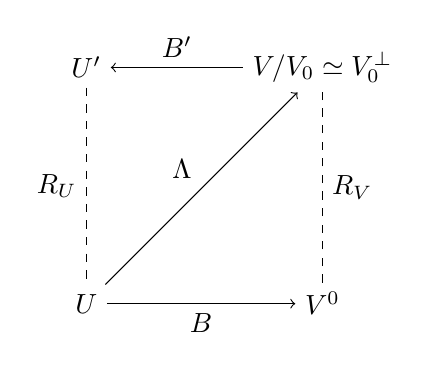
\begin{tikzpicture}
      [auto]
      \node(1) at (0, 0) {$U$};
      \node(2) at (3, 0) {$V^0$};
      \node(3) at (3, 3) {$V/V_0 \simeq V_0^\perp$};
      \node(4) at (0, 3) {$U^\prime$};
      \draw[->](1) --node[below]{$B$} (2);
      \draw[dashed](2) --node[right]{$R_V$} (3);
      \draw[->](3) --node[above]{$B^\prime$} (4);
      \draw[dashed](4) --node[left]{$R_U$} (1);
      \draw[->](1) --node[above left]{$\Lambda$} (3);
  \end{tikzpicture}
\end{center}

其中$V_0 = N(B^\prime)$,$V^0$为$V_0$的零化子空间,限制之后$R_V$仍是等距同构。

现在回过头来,对于自反Banach空间
\begin{center}
  \begin{tikzpicture}
      [auto]
      \node(1) at (0, 0) {$U$};
      \node(2) at (3, 0) {$V^\prime$};
      \node(3) at (3, 3) {$V$};
      \node(4) at (0, 3) {$U^\prime$};
      \node(5) at (-3, 0) {$U^{\prime \prime}$};
      \node(6) at (6, 3) {$V^{\prime \prime}$};
      \draw[->](1) --node[below]{$B$} (2);
      \draw[->](3) --node[above]{$B^\prime$} (4);
      \draw[dashed](2) -- (3);
      \draw[dashed](1) -- (4);
      \draw[->](1) --node[below]{$J_U$} (5);
      \draw[->](3) --node[above]{$J_V$} (6);
      \draw[dashed](4) -- (5);
      \draw[dashed](2) -- (6);
      \draw[<->] (-0.3, 1.5) --node[below]{\scriptsize{Reflexive}} (-1.2, 1.5);
      \draw[<->] (3.3, 1.5) --node[above]{\scriptsize{Reflexive}} (4.2, 1.5);
  \end{tikzpicture}
\end{center}

Conjugate in Banach, Adjoint in Hilbert

对于协调元离散问题:给定$U_{h} \subset U, V_{h} \subset V$,找$u_{h} \in U_{h}$ s.t.
\[
  b(u_{h}, v_{h})=\langle f, v_h\rangle_{V^{\prime} \times V}, \quad \forall v_{h} \in V_{h}
\]

离散问题的适定性. 只需下述离散的inf-sup条件成立
\[
  \text{d. } \qquad \inf_{u_{h} \in U_{h}} \sup _{v_{h} \in V_{h}} \frac{b\left(u_{h}, v_{h}\right)}{\left\|u_{h}\right\|_{U}\left\|v_{h}\right\|_{V}}=\inf_{v_{h} \in V_{h}} \sup _{u_{h} \in U_{h}} \frac{b\left(u_{h}, v_{h}\right)}{\left\|u_{h}\right\|_{U}\left\|v_{h}\right\|_{V}}=\beta_{h}>0 
\]

对于对称情形(Lax-Milgram定理),连续问题的适定性蕴含离散问题的适定性,但是对于非对称情形(Babuška引理)不成立,简单来说有界性和强制性是可以继承得到,但是inf-sup常数限制在小空间上就不一样了,一般来说$\beta_h \le \beta$。

误差估计:若a. + b. + c. + d. 成立,则连续和离散问题的解都是存在唯一的,且有估计
\[
  \left\|u-u_{h}\right\|_{U} \le \left(1+\frac{M}{\beta_{h}}\right) \inf _{w_{h} \in U_{h}}\left\|u-w_{h}\right\|_{U}
\]

引入投影算子$P_h: U \to U_h$ s.t. $b(u, v) = b(P_h u:=u_h, v)$,则有
\[
  \begin{aligned}
    \|u - u_h\|_U &= \|(I - P_h)u\|\\
    &=\|(I - P_h)(u - w_h)\|\\
    &\le \|I - P_h\|_{op} \|u - w_h\|_U\\
    &\le (1 + \|P_h\|_{op}) \inf_{w_h \in U_h} \|u - w_h\|_U
  \end{aligned}
\]

对于Hilbert空间中的投影算子有$\|I - P\|_{op} = \|P\|_{op}$(see Demkowicz's Notes),于是
\[
  \|u - u_h\|_U \le \|P_h\|_{op} \inf_{w_h \in U_h} \|u - w_h\|_U
\]

其中由$\beta_h \|P_h u\|_U = \sup_{v_h \in V_h} \frac{|b(P_h u, v_h)|}{\|v_h\|}= \sup_{v_h \in V_h} \frac{|b(u, v_h)|}{\|v_h\|} \le M \|u\|_U$,故$\|P_h\|_{op} \le \frac{M}{\beta_h}$。

\subsubsection{Brezzi理论}

鞍点问题连续情形:求$u \in V, p \in Q$ s.t.
\[
  \left\{\begin{array}{ll}
    a(u, v)+b(v, p)=\langle f, v\rangle_{V^{\prime} \times V} & \forall v \in V \\
    b(u, q)=\langle g, q\rangle_{Q^{\prime} \times Q} & \forall q \in Q
  \end{array}\right.
\]

其中$a(\cdot, \cdot): V \times V \to \mathbb{R}, b(\cdot, \cdot): V \times Q \to \mathbb{R}$。

\begin{enumerate}[a.]\setcounter{enumi}{4}
  \item $a(v, v) \ge \alpha\|v\|_{V}^{2}, \quad \forall v \in V_{0}$
  
  即$a(\cdot, \cdot)$在$V_0$上强制,故$A$下有界,$A^\prime$商核后下有界。
  \item $\sup _{0 \neq v \in V} \frac{b(v, q)}{\|v\|_{V}} \geq \beta\|q\|_{Q}, \quad \forall q \in Q$
  
  即$B^\prime$下有界,商左边。
\end{enumerate}

则上述连续问题存在唯一解,且有估计
\[
  \|u\|_{V}+\|p\|_{Q} \le C\left(\|f\|_{V^{\prime}}+\|g\|_{Q^{\prime}}\right)
\]

\begin{center}
  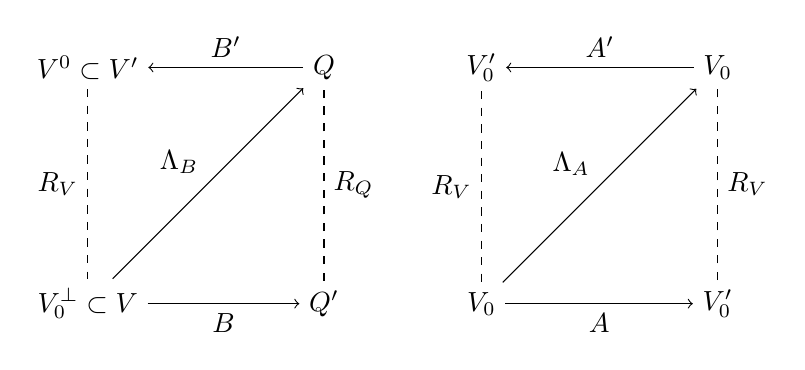
\begin{tikzpicture}
      [auto]
      \node(1) at (0, 0) {$V_0$};
      \node(2) at (3, 0) {$V_0^\prime$};
      \node(3) at (3, 3) {$V_0$};
      \node(4) at (0, 3) {$V_0^\prime$};
      \draw[->](1) --node[below]{$A$} (2);
      \draw[dashed](2) --node[right]{$R_V$} (3);
      \draw[->](3) --node[above]{$A^\prime$} (4);
      \draw[dashed](4) --node[left]{$R_V$} (1);
      \draw[->](1) --node[above left]{$\Lambda_A$} (3);

      \node(5) at (-5, 0) {$V_0^\perp \subset V$};
      \node(6) at (-2, 0) {$Q^\prime$};
      \node(7) at (-2, 3) {$Q$};
      \node(8) at (-5, 3) {$V^0 \subset V^\prime$};
      \draw[->](5) --node[below]{$B$} (6);
      \draw[dashed](6) --node[right]{$R_Q$} (7);
      \draw[->](7) --node[above]{$B^\prime$} (8);
      \draw[dashed](8) --node[left]{$R_V$} (5);
      \draw[->](5) --node[above left]{$\Lambda_B$} (7);
  \end{tikzpicture}
\end{center}

原问题等价于算子方程
\[
  \left\{\begin{array}{ll}
    Au + B^\prime p = f\\
    Bu = g
  \end{array}\right.
\]

pf: 令$V_0 = N(B)$,先由第二个方程的Babuška理论(图1)得到$u_g \in V_0^\perp$以及估计
\[
  \|u_g\|_V \le C\|g\|_{Q^\prime}
\]

再将第一个方程限制在$V_0$上,此时左边第二项消失且$f - Au \in V^0$,由Babuška理论(图2)得到$u_0 = u - u_g \in V_0$以及估计
\[
  \|u_0\|_V \le C\|f - Au_g\|_{V^\prime} \le C\|f\|_{V^\prime} + C\|u\|_V
\]

于是$u = u_g + u_0 \in V$。最后由第一个方程的Babuška理论(图1)得到p以及估计
\[
  \|p\|_Q \le C\|f - Au\|_{V^\prime} \le C\|f\|_{V^\prime} + C\|u\|_V
\]

综上结合$\|u\|_V \le \|u_g\|_V + \|u_0\|_V$可得
\[
  \|u\|_V + \|p\|_Q \le C(\|f\|_{V\prime} + \|g\|_{Q^\prime})
\]

离散问题

给定协调元空间$V_{h} \subset V, Q_{h} \subset Q$,离散问题为:求$u_{h} \in V_{h}, p_{h} \in Q_{h}$ s.t.
\[
  \left\{\begin{array}{ll}
    a\left(u_{h}, v_{h}\right)+b\left(v_{h}, p_{h}\right)=\left\langle f, v_{h}\right\rangle_{V^{\prime} \times V} \quad & \forall v_{h} \in V_{h} \\
    b\left(u_{h}, q_{h}\right)=\left\langle g, q_{h}\right\rangle_{Q^{\prime} \times Q} \quad & \forall q_{h} \in Q_{h}
  \end{array}\right.
\]

若条件e. 和f. 的离散版本$e_h.$ 和$f_h.$(LBB条件)成立,则离散问题解的适定性成立,且有误差估计
\[
  \left\|u-u_{h}\right\|_{v}+\left\|p-p_{h}\right\|_{Q} \leq C\left(\inf _{v_{h} \in V_{h}}\left\|u-v_{h}\right\|_{V}+\inf _{q_{h} \in Q_{h}}\left\|p-q_{h}\right\|_{Q}\right)
\]

pf: 由Galerkin正交性(误差方程)和离散问题解的适定性,见ppt FEM-10 p2。

对于离散问题可以把双线性泛函看成二次型$b_h(u_h, v_h) = u_h^T B v_h$,此时验证LBB条件即估计矩阵B的最小/最大特征值,一般来说这是困难的,于是引入LBB条件的一个充分条件,即Fortin准则。

\begin{thm}
  (Fortin准则)若双线性泛函$b: V \times Q \to \mathbb{R}$满足inf-sup条件,且对于协调元空间$V_h, Q_h$存在有界线性算子$\Pi_h: V \to V_h$ s.t.
  \[
    \begin{aligned}
      b(\Pi_h v, q_h) = b(v, q_h),& \quad \forall q_h \in Q_h\\
      \|\Pi_h v\|_V \le \|v\|_V,& \quad \forall v \in V
    \end{aligned}
  \]

  其中C与h无关(由$C \sim \frac{1}{\beta_h}$,说明离散inf-sup常数$\beta_h$与h无关),则LBB条件成立
\end{thm}

pf:
\[
  \begin{aligned}
    \beta\left\|q_{h}\right\|_{Q} & \leq \sup _{v \in V} \frac{b\left(v, q_{h}\right)}{\|v\|_{V}}=\sup _{v \in V} \frac{b\left(\Pi_{h} v, q_{h}\right)}{\|v\|_{V}} \\
    & \le C \sup _{v \in V} \frac{b\left(\Pi_{h} v, q_{h}\right)}{\left\|\Pi_{h} v\right\|_{V}} \leq C \sup _{v_{h} \in V_{h}} \frac{b\left(v_{h}, q_{h}\right)}{\left\|v_{h}\right\|_{V}}
  \end{aligned}
\]

-----Poisson问题
\[
  \begin{array}{l}
    V = H(\operatorname{div}, \Omega), \quad Q = L^2(\Omega), \quad V_0 = N(\operatorname{div})\\
    a(\undertilde{p}, \undertilde{q})=\int_{\Omega} \undertilde{p} \cdot \undertilde{q} dx, \quad b(\undertilde{q}, v)=\int_{\Omega} \operatorname{div} \undertilde{q} v dx
  \end{array}
\]

验证Brezzi理论条件:
\begin{enumerate}
  \item 有界性即Cauchy-Schwarz不等式。
  \item e. $a(\undertilde{p}, \undertilde{p}) = \sum_i\|p_i\|_{0, \Omega}^2 = \|\undertilde{p}\|_{0, \Omega}^2 = \|\undertilde{p}\|_{\operatorname{div}, \Omega}^2, \forall \undertilde{p} \in V_0$($\|\undertilde{p}\|_{\operatorname{div}, \Omega} = \|\undertilde{p}\|_{0, \Omega} + \|\operatorname{div} \undertilde{p}\|_{0, \Omega}$)
  \item f. 利用Poisson方程构造性证明:(构造性就是找一个成立)
  
  考虑Dirichlet边值条件的Poisson问题$\left\{\begin{array}{l}
    -\Delta \phi=q \\
    \phi|_{\partial \Omega}=0
  \end{array}\right.$,取$\undertilde{p} = - \nabla \phi \in H(\operatorname{div}, \Omega)$,则
  \[
    \begin{aligned}
      &(\operatorname{div} \undertilde{p}, q)=(-\operatorname{div} \nabla \phi, q)=(q, q)=\|q\|_{0, \Omega}^{2}\\
      &\|\undertilde{p}\|_{\operatorname{div}, \Omega}^{2}=\|\undertilde{p}\|_{0, \Omega}^{2}+\|\operatorname{div} \undertilde{p}\|_{0, \Omega}^{2}=\|\nabla \phi\|_{0, \Omega}^{2}+\|q\|_{0, \Omega}^{2} \leq C\|q\|_{0, \Omega}^{2} 
    \end{aligned}
  \]

  最后一个不等号是由正则性$\|\phi\|_{1, \Omega} \leq C\|g\|_{-1, \Omega} \leq C\|q\|_{0, \Omega}$。于是
  \[
    \sup_{0 \neq \undertilde{p} \in V} \frac{(\operatorname{div} \undertilde{p}, q)}{\|\undertilde{p}\|_{\operatorname{div}, \Omega}} \ge \frac{\|q\|_{0, \Omega}^2}{\sqrt{C}\|q\|_{0, \Omega}} = \frac{1}{\sqrt{C}}\|q\|_{0, \Omega}, \quad \forall q \in Q
  \]
\end{enumerate}

-----Stokes问题
\[
  \begin{array}{l}
    V = \left(H_0^1(\Omega)\right)^d, \quad Q = L_0^2(\Omega), \quad V_0 = N(\operatorname{div})\\
    a(\undertilde{u}, \undertilde{v})=\int_{\Omega} \nabla \undertilde{u}: \nabla \undertilde{v} dx, \quad b(\undertilde{v}, q)=-\int_{\Omega} \operatorname{div} \undertilde{v} q dx
  \end{array}
\]

验证Brezzi理论条件
\begin{enumerate}
  \item 有界性
  \item e. 由Poincaré不等式,$a(\undertilde{u}, \undertilde{u}) = \|\nabla \undertilde{u}\|_0 \ge \|u\|_1, \forall \undertilde{u} \in V$
  \item f. 考虑二维区域且边界是凸的或充分光滑。构造性证明:
  
  注意到$\operatorname{div}: V \to L_0^2(\Omega)$是满的,$\forall q \in L_0^2(\Omega), \exists \undertilde{v} \in V, -\operatorname{div} \undertilde{v} = q$,再设$\undertilde{v} = \operatorname{grad}\phi, \phi \in H^1(\Omega)$,于是$-\Delta \phi = q$。

  要想$\undertilde{v} = \nabla \phi \in V = (H_0^1(\Omega))^2$,需要$\nabla \phi \cdot \nu|_{\partial \Omega} = \nabla \phi \cdot \tau|_{\partial \Omega} = 0$,第一个条件直接加在$\phi$上,可得Neumann边值条件的Poisson问题$\left\{\begin{array}{l}
    -\Delta \phi=q \\
    \nabla \phi \cdot \nu|_{\partial \Omega}=0
  \end{array}\right.$。再去修正切向导数,为了不破坏Poisson问题,设$\left\{\begin{array}{l}
    \undertilde{w} = \operatorname{curl} \psi\\
    \psi|_{\partial \Omega} = 0\\
    \nabla \psi \cdot \nu|_{\partial \Omega} = - \nabla \phi \cdot \nu|_{\partial \Omega}
  \end{array}\right.$。故$\undertilde{u} = \undertilde{v} + \undertilde{w} \in V, \operatorname{div}\undertilde{u} = q$,由$\phi, \psi \in H^2(\Omega)$可得正则性$\|\undertilde{v}\|_{1, \Omega} \le C\|q\|_{0, \Omega}$以及$\|\undertilde{w}\|_{1, \Omega} \le C\|v\|_{0, \Omega}$。于是
  \[
    \sup_{0 \neq \undertilde{p} \in V} \frac{(\operatorname{div} \undertilde{p}, q)}{\|\undertilde{p}\|_{1, \Omega}} \ge \frac{(\operatorname{div} \undertilde{u}, q)}{\|\undertilde{u}\|_{1, \Omega}} \ge C\|q\|_{0, \Omega}, \quad \forall q \in Q
  \]
  



  
  一般区域上的结论和正则性见Girault, Raviart。
\end{enumerate}

----- Stokes问题的有限元离散

$P_2 - P_0$元
\[
  \begin{array}{l}
    S_{h}=\left\{v_{h} \in H^{1}(\Omega) \mid v_{h}|_{K} \in P_{2}(K), \forall K \in \mathcal{T}_{h}\right\} \text{ (Lagrange二次元)}\\
    M_{h}=\left\{q_{h} \in L^{2}(\Omega) \mid q_{h}|_{K} \in P_{0}(K), \forall K \in \mathcal{T}_{h}\right\} \text{ (分片常数)}\\
    V_{h}=\left(S_{h} \cap H_{0}^{1}(\Omega)\right)^{2}, Q_{h}=M_{h} \cap L_{0}^{2}(\Omega)
  \end{array} 
\]

定义$\Pi_h^1: H_0^1(\Omega) \to S_h \cap H_0^1(\Omega)$为Lagrange二次元的Scott-Zhang插值,则有插值误差估计
\[
  \left\|\undertilde{v}-\Pi_{h}^{1} \undertilde{v}\right\|_{0, K}+h_{K}|\undertilde{v}-\Pi_{h}^{1} \undertilde{v}|_{1, K} \le h_{K}|\undertilde{v}|_{1, \omega_{K}}
\]

但是$\Pi_h^1$不是可交换的,即不满足Fortin准则1. ,于是引入插值$\Pi_h^2$进行修正
\[
  \left\{\begin{array}{l}
    \Pi_{h}^{2} v\left(a_{i}\right)=0, \quad i = 1, 2, 3 \\
    \int_{e_{i}} \Pi_{h}^{2} v \mathrm{ds}=\int_{e_{i}} v \mathrm{ds}, \quad i = 1, 2, 3
  \end{array}\right.
\]

若有可交换性$b(v - \Pi_h v, q_h) = 0, \forall q_h \in Q_h$,则$\sum_K \int_K \operatorname{div}(v - \Pi_h v) q_h dx = \sum_K q_h \int_K \operatorname{div}(v - \Pi_h v) dx = 0$,故只需要$\int_K \operatorname{div}(v - \Pi_h v) dx = 0, \forall K$,其中最后一个等号是因为$q_h \in Q_h$是分片常数。

其有界性(HW 10.3)
\[
  \left\|\Pi_{h}^{2} \undertilde{v}\right\|_{0, K} \le C\left(\|\undertilde{v}\|_{0, K}+h_{K}|\undertilde{v}|_{1, K}\right)
\]

构造Fortin插值$\Pi_h$ s.t. $I - \Pi_h = (I - \Pi_h^2)(I - \Pi_h^1)$。把$(I - \Pi_h^1)v$看成一个整体,则$\Pi_h$是可交换的。
\[
  \begin{aligned}
    \left|\Pi_{h} \undertilde{v}\right|_{1, \Omega}^{2} & \le \left|\Pi_{h}^{1} \undertilde{v}\right|_{1, \Omega}^{2}+\left|\Pi_{h}^{2}\left(\undertilde{v}-\Pi_{h}^{1} \undertilde{v}\right)\right|_{1, \Omega}^{2}\\
    & \le C|\undertilde{v}|_{1, \Omega}^{2}+C \sum_{K \in \mathcal{T}_{h}} h_{K}^{-2}\left\|\Pi_{h}^{2}\left(\undertilde{v}-\Pi_{h}^{1} \undertilde{v}\right)\right\|_{1, K}^{2}\\
    & \le C|\undertilde{v}|_{1, \Omega}^{2}+C \sum_{K \in \mathcal{T}_{h}}\left(h_{K}^{-2}\left\|\undertilde{v}-\Pi_{h}^{1} \undertilde{v}\right\|_{0, K}^{2}+\left|\undertilde{v}-\Pi_{h}^{1} \undertilde{v}\right|_{1, K}^{2}\right)\\
    & \le C|\undertilde{v}|_{1, \Omega}^{2}
  \end{aligned}
\]

分别是:三角不等式,Scott-Zhang插值有界性和逆估计,$\Pi_h^2$有界性,Scott-Zhang插值误差估计。

最后有插值误差估计
\[
  \left\|\undertilde{u}-\undertilde{u}_{h}\right\|_{1, \Omega}+\left\|p-p_{h}\right\|_{0, \Omega} \leq C\left(\inf_{\undertilde{v}_{h} \in V_{h}}\left\|\undertilde{u}-\undertilde{v}_{h}\right\|_{1, \Omega}+\inf _{q_{h} \in Q_{h}}\left\|p-q_{h}\right\|_{0, \Omega}\right)
\]

若$\undertilde{u} \in\left(H^{2}(\Omega)\right)^{2}, p \in H^{1}(\Omega)$,则由估计插值误差估计可得
\[
  \left\|\undertilde{u}-\undertilde{u}_{h}\right\|_{1, \Omega}+\left\|p-p_{h}\right\|_{0, \Omega} \leq C\left(h^{2}|\undertilde{u}|_{2, \Omega}+h|p|_{1, \Omega}\right)
\]

h的阶数出自Lagrange二次元的$H^1$误差估计和分片常数的$L^2$误差估计。

\section{后验误差估计}

\newpage

\section{一些}
一些映射:
\begin{enumerate}
  \item 插值算子:$\Pi_K: C^\ell(K) \to W^{m, p}(K), \Pi_K u = \sum_i N_i(u) \Phi_i$
  \item 投影算子:$P_m: W^{m, p}(\Omega) \to P_m(\Omega)$
\end{enumerate}

一些不等式:
\begin{enumerate}
  \item 1. Young不等式: $a b \le \frac{1}{p} a^{p}+\frac{1}{q} b^{q}$. (a, b $\ge$ 0 in case you dont know)

  2. Holder不等式: $\|f \cdot g\|_{0, 1, \Omega} \le\|f\|_{0, p, \Omega}\|g\|_{0, q, \Omega}$. Proof by Young不等式.
  
  3. Minkowski不等式: $\|f+g\|_{0, p, \Omega} \le\|f\|_{0, p, \Omega}+\|g\|_{0, p, \Omega}$.
  \item Sobolev空间中的范数等价定理
  \begin{enumerate}
    \item Poincaré-Friedrichs不等式:
    \[
      \|v\|_{m, \Omega} \le C_{1}|v|_{m, \Omega}, \forall v \in H_{0}^{m}(\Omega).
    \]
    \item Poincaré不等式:
    \[
      \|v\|_{m, \Omega}^{2} \le C_{2}\left(|v|_{m, \Omega}^{2}+\sum_{|\alpha|<m}\left(\int_{\Omega} \partial^{\alpha} v dx\right)^{2}\right), \forall v \in H^{m}(\Omega).
    \]
    m = 1时:
    \[
      \|v\|_{1, \Omega}^{2} \le C_{2}\left(|v|_{1, \Omega}^{2}+\left(\int_{\Omega} v dx\right)^{2}\right), \forall v \in H^{1}(\Omega).
    \]
  \end{enumerate}
  \item Poincaré不等式:
  \[
    \left\|u-(u)_{U}\right\|_{0, p, U} \le C\|D u\|_{0, p, U} = C\sum_{i} \|\partial_i u\|_{0, p, U}, \forall u \in W^{1, p}(U).
  \]
\end{enumerate}

一些估计:
\begin{enumerate}[]
  \item 几何估计:$\|B\| \le \frac{h_{K}}{\rho_{\widehat{K}}},|\operatorname{det} B| \le C\left(\frac{h_{K}}{\rho_{\widehat{K}}}\right)^{n}$。
  \item 单元估计:$|\widehat{v}|_{m, p, \widehat{K}} \le C\|B\|^{m}|\operatorname{det} B|^{-1 / p}|v|_{m, p, K}$。
  \item 单元边界估计:$\|\widehat{v}\|_{0, p, \partial \widehat{K}} \le C\|B\|^{1 / p}|\operatorname{det} B|^{-1 / p}\|v\|_{0, p, \partial K}$。
  \item Verfürth投影估计:$\left\|u-P_{k} u\right\|_{k+1, p, \Omega} \le C(m, n, \gamma)|u|_{k+1, p, \Omega}$。
  \item 局部插值误差估计:$\|v - \Pi_K v\|_{i, p, K} \le C h^{m - i} \|v\|_{m, p, K}$
  \item 整体插值误差估计:$\left(\sum_{K \in \mathcal{T}_{h}}\left\|v-\Pi_{K} v\right\|_{s, p, K}^{p}\right)^{1 / p} \le C h^{m-s}|v|_{m, p, \Omega}$。
  \item 局部逆估计:$\|v\|_{\ell, p, K} \le C h^{m-\ell+n / p-n / q}\|v\|_{m, q, K}$。
  \item 整体逆估计:
\end{enumerate}

一些题目:

证明基本不等式

证明空间完备性

求弱形式

证明弱解在一定正则性下就是古典解





一些技巧:

空间稠密性

反证法

算子角度

一些问题:285

flag


\vspace{5pt} \hrule \vspace{5pt}

\chapter{FA}

\section{拓扑线性空间}

\subsection{Topology of TLS}
四菜一汤:代数结构(线性结构,群环域),拓扑结构(拓扑,度量,范数,内积),测度结构(可积先可测),序结构。

TLS:线性和拓扑空间,且加法和数乘(作为乘积拓扑空间到拓扑空间的映射)连续,即线性结构与拓扑结构相容。

1. $T_{\lambda, a}: X \to X, T_{\lambda, a}(x) = \lambda x + a, \lambda \in \mathbb{K}, a \in X$是拓扑同胚。

2. TLS is T2 and T3.

邻域:包含(包含点的)开集。邻域全体$\mathcal{N}(x)$。

邻域基:每个邻域都能找到更小的邻域基中的元素(仍为邻域)含于其中。(这里不需要说是谁的邻域基,因为TLS中有线性结构,因此有平移操作,任意一点处的邻域基可以由零点处的邻域基所生成,类似Lie群)考虑零点的邻域基$\mathcal{U}(\theta)$,则$\forall a \in X$的邻域可以表示成$a + U, U \in \mathcal{U}(\theta)$,进一步$V + U = \cup_{a \in V} (a + U)$是开的。两个TLS相同,若其邻域基相容,即邻域基之于TLS相当于拓扑基之于TS,事实上邻域基完全决定了TLS的拓扑。

NLS的零点的邻域基为单点基$\{ B(0, 1) \}$。(这是因为有范数)以这个单位球为起点,定义:

(a). 吸收集:$\forall x \in \textbf{X}, \exists \alpha \textbf{>} 0 \text{ s.t. } \forall |\lambda| \le \alpha, \lambda x \in S$(包含\textbf{X中}任意一点确定的仿射线段的某个伸缩)

(b). 平衡集:$\forall s \in \textbf{S}, \forall \alpha \in \mathbb{K}, |\alpha| \le 1 \text{ s.t. }  \alpha s \in S$(包含\textbf{S中}任意一点确定的仿射线段)平衡包$\bar{S}^b = \{ \alpha s | |\alpha| \le 1, s \in S \}$。(包含S的最小闭球)

(c). 凸集:$\forall \alpha \in [0, 1], \alpha S + (1 - \alpha) S \subset S$。(主打一个入乡随俗)平衡凸 = 平衡 + 凸。凸包$\bar{S}^c$。(包含S的最小凸集)平衡凸包$\bar{S}^{bc} = \overline{\bar{S}^b}^c \neq \overline{\bar{S}^c}^b$。(包含S的最小平衡凸集)(一个例子:考虑x轴和y轴正半轴构成的空间,先取平衡包是整个x轴和y轴,再取凸包是全空间,先取凸包是第一象限,再取平衡包是一三象限)

注:关于数乘,在实数域表示伸缩,在复数域表示旋转和伸缩,所以在讨论问题的时候必须先说好是实数域还是复数域,在实数域用旋转和伸缩就乱套了,事实上上面很多就是,你说的闭球什么的就都是错的。旋转是说复数域里面的伸缩放到实数域里面看有旋转的效果,这个定义想说的还是伸缩下的性质,就是仿射性质。写这个注是受到一个例子的启发。

平衡集但不是凸集的例子:考虑实数域:$\{(x, y) \in \mathbb{R}^2 | xy = 0\}$,即x轴加y轴,显然是平衡的,不是凸的。考虑复数域把$\mathbb{R}$换成$\mathbb{C}$就好了,那就是$\mathbb{C}^2 \cong \mathbb{R}^4$了。

于是我们只需要考虑实数域和伸缩就好了。

\begin{prop}
  1. 任意吸收集包含零点,但$\{ \theta \}$不吸收。(因为伸缩系数为正)

  2. 任意零点的邻域是吸收的。(零点的邻域必然包含某个$B(0, \varepsilon)$,伸缩系数取$\varepsilon$(不是零!)即可,这里使用了数乘的连续性)反之并不成立,反例:$[-2, -1) \cap \{0\} \cap (1, 2]$。

  3. 若S平衡,则S吸收 iff $\forall x \in X, \exists \alpha \neq 0, \alpha x \in S$.(平衡所以不用考虑旋转,只要存在一致的伸缩系数就好了)

  4. 平衡集的闭包是平衡的。

  5. 若平衡集的内核包含零点,则内核是平衡的。(pf by def,内核是最大开集)

  6. 凸集的内核和闭包都是凸的。

  7. 吸收集/平衡集/凸集的线性组合仍是吸收集/平衡集/凸集。

  8. $\alpha, \beta \ge 0$,S凸$\Rightarrow$ $\alpha S + \beta S = (\alpha + \beta)S$。(证相互包含)
\end{prop}

\begin{thm}
  TLS上存在“好”的邻域基$\mathcal{U}$,满足:

  1. $\forall U \in \mathcal{U}$吸收且平衡。

  2. 裂变:$\forall U \in \mathcal{U}, \exists V 
  \in \mathcal{U}$ s.t. $V + V \subset U$.

  3. $\forall U_1, U_2 \in \mathcal{U}, \exists U_3 \in \mathcal{U}$ s.t. $U_3 \subset U_1 \cap U_2$.
  
  反之,若线性空间X的子集族$\mathcal{V}$满足以上三条,则存在唯一X上的拓扑使得X构成TLS,并且$\mathcal{V}$为邻域基。这说明以上三条完全刻画了X的拓扑。
\end{thm}

\begin{pf}
  $\Rightarrow$ 令$\mathcal{U} = \{ \bar{U}^b | U \in \mathcal{N}(\theta) \}$。

  0. 先证$\mathcal{U}$确实一个邻域基,即证零点的任意邻域包含更小的平衡邻域,需要使用数乘的连续性。

  1. 吸收:包含吸收集的集合吸收。平衡:显然。

  2. 裂变:使用加法的连续性,$\exists U_1, U_2 \in \mathcal{U}$ s.t. $U_1 + U_2 \subset U$,令$V = U_1 \cap U_2$即可,要证V是平衡的。

  3. 使用数乘的连续性,令$W = U_1 + U_2$, $V = \cup_{\lambda \le \delta} \lambda W$,先证$W \in \mathcal{U}$,再证V是平衡的。(其实直接由邻域基就可以得到)

  $\Leftarrow$ 令$\mathcal{N}(x) = \{ V \subset X | \exists U \in \mathcal{U} \text{ s.t. } x + U \subset V \}$,S为开集($S \in \mathcal{O}(X)$)若$\forall s \in S, S \in \mathcal{N}(s)$.

  1. 证拓扑空间,即验证三条:空集和全集,任意并封闭,有限交(两个交)封闭。

  2. 证TLS,即证加法和数乘连续。(TLS上的线性算子,在一点处连续等价于连续等价于一致连续。但是这里就是要证TLS啊,还是得证任意一点)

  加法:$m: X \times X \to X, m(x, y) = x + y$,证在$(x, y)$处连续即证$\forall U \in \mathcal{U}, \exists U_1, U_2 \in \mathcal{U}$ s.t. $x + U_1 + y + U_2 \subset x + y + U$,由裂变令$U_1 = U_2 = V$即可。

  数乘:$p: \mathbb{K} \times X \to X, p(\alpha, x) = \alpha x$,证在$(\alpha, x)$处连续即证$\forall U \in \mathcal{U}, \exists \delta > 0, U_1 \in \mathcal{U}$ s.t. $\forall |\lambda| \le \delta, (\alpha + \lambda)(x + U_1) \subset \alpha x + U$。先用裂变和平衡证一个引理:$\forall U \in \mathcal{U}, \alpha \neq 0, \exists V \in \mathcal{U}$ s.t. $\alpha V \subset U$,再用裂变,让加一项减一项之后得到的两部分都在裂变的V里面。

  3. 证邻域基,由构造过程显然。

  4. 证(拓扑的)唯一性,拓扑由邻域基唯一确定。
\end{pf}

\begin{conc}
  \textbf{(Week 1)} TLS,邻域基,abc,TLS上存在好的邻域基:平衡吸收,裂变,交性质,邻域基决定拓扑。总之是:什么是TLS?
\end{conc}

关键词:球,弱,界。

\subsection{局部凸空间}

若S是凸或平衡凸的,则S的内核以及闭包都是凸或平衡凸的。

pf: 把内核和闭包理解为最大开集和最小闭集,由定义即可。

注:abc是线性性质,内核和闭包是拓扑性质,所以这里X是TLS。

\begin{thm}
  TLS X,若U是凸邻域,则U包含一个开的平衡凸的邻域基,即凸邻域能被开的平衡凸的邻域基(平衡吸收,裂变,交性质)生成。这样在讨论局部凸空间的时候,我们的邻域基就更好了。
\end{thm}

回到那个问题:什么时候TLS能成为NLS?我们已经知道了什么是TLS,那么什么时候能成为NLS,这时候需要局部凸空间。此时,邻域基有更好的性质,更像一个NLS的邻域基,也就是单位\textbf{球}。

这里邻域基和邻域基中的元素就按照语意自己区分一下吧。

pf: 取邻域基$V \subset U$,则$\tilde{V} = (\bar{V}^c)^{\circ}$即为所求。要证$\tilde{V}$仍为邻域基(by def),以及$\tilde{V} \subset U$(凸包是最小凸集)。

局部凸空间(LCS):若邻域基中元素全是凸集。

对于球,我们想要知道其半径,于是引入“尺子”。

LS X上的半范数$p: X \to \mathbb{R}$ if

1. 正性:$p(x) \le 0$。

2. 齐性:$p(\lambda x) = |\lambda| p(x)$。

3. 三角不等式:$p(x + y) \le p(x) + p(y)$。

范数 if 定。

由于p是从X到$\mathbb{R}$的映射,我们可以将X中的那些类球邻域和真正的球进行比较。令$V_1 = p^{-1}([0, 1)) = \{x \in X | p(x) < 1\}, V_2 = p^{-1}([0, 1]) = \{x \in X | p(x) \le 1\}$,则$V_1, V_2$都是abc的。(若$X = \mathbb{R}^n$,则$V_1 = B(0, 1), V_2 = D(0, 1)$)

pf: ab由齐性,c由三角不等式。

TLS X,有了拓扑,我们讨论p的连续性:p连续 iff $V_2 \in \mathcal{N}(\theta)$。

pf: $\Rightarrow$ 显然。 $\Leftarrow$ by def: $\forall \varepsilon > 0, \exists \frac{1}{2} \varepsilon N_2 \in \mathcal{N}(\theta)$ s.t. $p(x) \le \frac{1}{2} \varepsilon < \varepsilon$. (这里是说在原点处连续,在任意一点处类似)

\begin{thm}
  LS X,$\mathcal{P}$是其上的一族半范数,令$V(p) = \{x \in X | p(x) < 1\}$,
  \[
    \mathcal{U} = \left\lbrace \bigcap_{i = 1}^n \gamma_i V(p_i) \bigg| n \in \mathbb{N}, \gamma_i \in \mathbb{K}, p_i \in \mathcal{P} \right\rbrace, 
  \]
  则$\mathcal{U}$是使得X成为LCS的邻域基(其中元素都是凸集),并且其诱导的拓扑$\tau$是使得所有p都连续的最小拓扑(最小拓扑是说,开集的个数最少)。
\end{thm}

pf: 1. 证$\mathcal{U}$是X上的邻域基:平衡吸收和分裂由$V(p)$的abc引理,交性质由构造(伸缩的有限交)。

2. 证$p$关于$\tau$连续:由上述连续性引理。

3. 证最小拓扑:设$\hat{\tau}$是使得X为LCS和所有p都连续的拓扑,则$V(p) \in \mathcal{N}_{\hat{\tau}}(\theta)$,于是其伸缩的有限交也属于后者,即$\mathcal{U} \subset \mathcal{N}_{\hat{\tau}}(\theta)$。

记$\tau := \langle \mathcal{P} \rangle$为由$\mathcal{P}$生成的局部凸拓扑。

$(X, \langle \mathcal{P} \rangle)$,则X是$T_2$的 iff $\forall x \in X, \exists p \in \mathcal{P}$ s.t. $p(x) \neq 0$(称可分点的).

pf: $\Rightarrow$ 由构造邻域基一定长成伸缩有限交的样子,$x \notin \gamma_i V(p_i) \Leftrightarrow p_i(x) > \gamma_i$ $\Leftarrow$ 显然。

LCS X, $(Y, \langle \mathcal{P} \rangle)$,则$T: X \to Y$连续 iff $\forall p \in \mathcal{P}, p \circ T: X \to \mathbb{R}$连续。

pf is omitted.(见刘培德p25定理4.5)

例子:1. 非空集合T,X为T上有界函数全体,$p_t(x) = |x(t)|$为X上的半范数,$\mathcal{P} = \{p_t, t \in T\} \Rightarrow \tau$,则$x_n \overset{\tau}{\to} x \Leftrightarrow \forall t \in T, |x_n(t) - x(t)| \to 0$,即逐点收敛。

2. TS T,X为T上连续函数全体,K为T中紧集,$p_K(x) = \max_{t \in K} |x(t)|$为X上的半范数,$\mathcal{P} = \{p_t, t \in T\} \Rightarrow \tau$,则$x_n \overset{\tau}{\to} x \Leftrightarrow \forall K \overset{compact}{\subset} T, \max_{t \in K} |x_n(t) - x(t)| \to 0$,即一致收敛。

3. B(H)上的弱算子拓扑和强算子拓扑?(博士资格考试)

\textbf{弱}:弱拓扑的弱体现在,由一族半范数生成的局部凸拓扑是最小的。(见夏道行p147定义3.3.7)

给定一族半范数可以诱导TLS上的局部凸拓扑,反过来由LCS上的拓扑能否构造一族半范数,使得其诱导的局部凸拓扑就是原来的拓扑?其难点在于如何构造这样的半范数族。

对于LS X上的ac集A,定义其上的Minkowski函数$p_A(x) = \inf \{ \lambda, x \in \lambda A \}, \forall x \in X$。若A还是b集,则$p_A$为X上的半范数。

pf is omitted.(见刘培德p5定理1.1)

对于上述ac集A,定义$A_1 = p_A^{-1}([0, 1)) = \{x \in X | p(x) < 1\}, A_2 = p_A^{-1}([0, 1]) = \{x \in X | p(x) \le 1\}$,则有$A^{\circ} \subset A_1 \subset A \subset A_2 \subset \bar{A}$。并且$p_A$连续蕴含着$\theta \in A^{\circ}$以及$A^{\circ} = A_1, A_2 = \bar{A}$。若A还是b集,则三者等价。(下面半范数族的连续性由此而来)

pf is omitted.(见刘培德p21引理4.3)

于是LCS X上的邻域基(其中元素都是abc集)上的Minkowski函数族即为想要的半范数族。这个半范数族又会诱导新的拓扑,两种拓扑的等价性证明见刘培德p23定理4.3注2。

(d). 有界集:$\forall U \in \mathcal{N}(\theta), \exists \lambda > 0$ s.t. $S \subset \lambda U$.

有界集的刻画:$S \subset X$有界 iff $\forall \{x_n\} \in S, \alpha_n \to 0(\mathbb{K})$, we have $\alpha_n x_n \to \theta(X)$.

pf is omitted.(见刘培德p13定理3.1)

可赋范化空间:若TS X上存在范数,使得该范数诱导的拓扑即为原来的拓扑。

Kolmogorov准则:TLS X是可赋范化的 iff X是T2的,且邻域基中元素是凸有界的。

\begin{conc}
  \textbf{(Week 2)} LCS,半范数,半范数族可以生成局部凸拓扑,弱拓扑,反过来LCS上也可以构造一族半范数,即邻域基元素上的Minkowski函数族,使得其诱导的局部凸拓扑就是原来的拓扑,Minkowski函数,有界集,Kolmogorov准则。

  还是那个问题:TLS什么时候是NLS?第一周讲的是什么是TLS,其由邻域基完全刻画,所以去研究邻域基。第二周讲的LCS,此时邻域基中的元素性质更好,更像是一个球。LCS由其上的一族半范数完全刻画,所以去研究半范数。还差一点有界性,TLS就是NLS了。
\end{conc}

球:形状:abc,数(半径):Minkowski函数。

弱拓扑:局部凸拓扑,使得一族半范都连续的最小拓扑

Kolmogorov准则:TLS X是可赋范化的 iff X是T2的,且存在凸有界的邻域基。

pf: 1. $\Leftarrow$ 令$U \in \mathcal{N}(\theta)$凸有界,$\exists V \subset U$平衡凸开有界,Minkowski函数$p_V$连续,为半范数。

2. 由U有界,$\forall W \in \mathcal{N}(\theta), \exists \alpha \ge 0$ s.t. $V \subset U \subset \alpha W \Rightarrow \{ \lambda V, \lambda \ge 0 \}$构成邻域基,此时$\langle p_V \rangle$生成的拓扑就是$\tau$。

3. 由T2,$x \neq \theta \Rightarrow p_V(x) \neq 0$,故$p_V$就是X上的范数。

另外TLS X什么时候是可度量化的,需要T1和邻域基可数。

一个例子:$X = C^{\infty}[0, 1], p_{n}(f) = \max_{t \in [0, 1]} |f^{(n)}(t)|$,$\{p_{n}\}$是一族半范数,X是可度量化的(可数),但不是可赋范化的。

\section{谱测度与谱分解}

\subsection{谱测度与谱积分}

分割求和取极限:$\left\{\begin{array}{ll}
  A = \sum_{i = 1}^{\infty} \lambda_n P_n \text{ (求和在强算子拓扑意义下收敛)} \\
  I = \sum_{i = 1}^{\infty} P_n
\end{array}\right.$

\subsubsection{谱测度}

两个空间:Hilbert空间H和集合X。$\mathcal{P}$是H上的投影算子族,$\mathcal{M}$是X上的$\sigma$-代数,映射$E: \mathcal{M} \to \mathcal{P}$,若

1. $E(X) = I$.

2. 可列可加性:$E(\cup_i A_i) = \sum_i E(A_i)$,$A_i \in \mathcal{M}$两两不交。

则称E为$(X, \mathcal{M})$上(H中)的谱测度,$(X, \mathcal{M}, E)$为H中的谱测度空间。

谱测度的性质:

1. 若$A, B \in \mathcal{M}$不交,则$E(A) E(B)=E(B) E(A)=0$。

2. 若$A, B \in \mathcal{M}$,则$E(A \cup B)=E(A)+E(B)-E(A \bigcap B)$(作为投影算子)。

3. $\{E(A) \mid A \in \mathcal{M}\}$是交换算子族.

谱测度诱导$(X, \mathcal{M})$上的测度:

1. $\mu_x(A) = \langle E(A)x, x \rangle$.

2. $\mu_{x, y}(A) = \langle E(A)x, y \rangle$.

这里$x, y \in H$是给定的,所以是不确定的,由此导出不同谱积分的定义。

用$\mathcal{M}(X)$表示X上可测函数全体,$B(X, \mathcal{M})$表示X上有界可测函数全体。

\subsubsection{谱积分}

定义$f \in B(X, \mathcal{M}), f: X \to \mathbb{K}$关于谱测度E的弱谱积分$T: B(X, \mathcal{M}) \to \mathcal{P}, T[f] = \int_X f(t) E(dt)$ s.t.
\[
  \langle \int_X f(t) E(dt) x, y \rangle = \int_X f(t) \langle E(dt) x, y \rangle
\]
i.e.,
\[
  \langle I[f]x, y \rangle = \int_X f(t) \mu_{x, y}(dt)
\]

弱谱积分的性质:

1. 1.5线性。

2. 压缩性:$\|I[f]\|_{H'} \le \|f\|_{\infty}$。

3. $E(A) = \int_X 1_A(t) E(dt)$.

pf: 2. 定义双线性泛函$\Phi(x, y) = \langle I[f]x, y \rangle$,对$\Phi(x, x)$用Riesz表示定理。

一致谱积分:按照值域分割求和取极限的过程定义。

两种谱积分本质上是等价的。

第一种定义比较简单,第二种是按照值域划分的过程来定义的,主要用于证明(建立积分)。

$\forall f, g \in B(X, \mathcal{M})$,$T[f]$与$T[g]$(作为投影算子)可交换(可换族)。

pf: 上面谱测度性质第三条相当于是说对于f和g是示性函数的时候上式成立,然后再按照测度论里面的思路,先对一个示性,简单,有界可测,然后再对另一个做就好了。(这里最大的空间就是有界可测函数就完了,没有一般可测)

$\forall f, g \in B(X, \mathcal{M})$,$T[f \cdot g] = T[f] \cdot T[g]$,乘法理解为函数乘法和投影算子复合。

pf: 示性,简单(线性),有界可测(控制收敛)。

\subsection{谱系}

$\mathbb{R}$上的测度与$\mathbb{R}$上单调递增的右连续函数一一对应。

$X = \mathbb{R}$上H中的谱测度与$X = \mathbb{R}$上单调递增的右连续投影算子值函数(谱系)一一对应。

\begin{df}(谱系)
  Hilbert空间H,$\{E_\lambda\}_{\lambda \in \mathbb{R}}$是一族投影算子,若有
  \begin{enumerate}
    \item 单调性:$\forall \lambda, \mu \in \mathbb{R}, \lambda \ge \mu$,有$E_{\lambda} \ge E_{\mu}$。(投影算子值域空间的单调性,越来越大)
    \item 右连续性:$\forall \lambda \in \mathbb{R}$,有(强)$E_{\lambda + 0} = E_\lambda$。
    \item 强算子拓扑收敛:(强)$\lim_{\lambda \to -\infty} E_{\lambda}=0$,(强)$\lim_{\lambda \rightarrow+\infty} E_{\lambda}=I$。
  \end{enumerate}
\end{df}

定义中的强收敛可以弱化为弱收敛。

谱系的充要条件(见夏道行实变与泛函下p287定理6.7.3$'$)

一个例子:$E_{\lambda} f=1_{(-\infty, \lambda]}(t) f(t), f \in H = L^{2}[0,1]$。

\subsection{有界自伴算子谱分解}

有界变差空间$BV[a, b] = \{g: [a, b] \to \mathbb{R} \mid g(a) = 0, g \text{ 右连续 }, \operatorname{Var}(g) < \infty\}$,其中,1. 左端点函数值为零和右连续称为规范化,是为了之后定义范数时的正定性。2. $\operatorname{Var}(g) = \sup_{\Delta} \operatorname{Var}(g, \Delta)$. 3. 有界变差则几乎处处可导。

\begin{lem}
  $C[0, 1]^{\ast} \cong BV[0, 1]$.
\end{lem}

pf: 令$\pi: BV[0, 1] \to C[0, 1]^{\ast}, \pi(g)(f) = \int_0^1 f(t) dg(t) = \int_0^1 f(t) g'(t) dt$(测度加权还是测度),则$\pi$是$BV[0, 1]$到$C[0, 1]^{\ast}$的等距同构。

\begin{lem}(唯一性引理)
  设$v \in BV[0, 1]$,若$\int_0^1 f(t) dv(t) = 0, \forall f \in C[0, 1]$,则$v = 0$。
\end{lem}

pf: n次方,多项式(线性),连续(Weierstrass定理 + 有界线性泛函)。

\begin{lem}
  令$u(t) = \int_0^t g(s) dv(s)$,则$\int_0^1 f(t) du(t) = \int_0^1 f(t) g(t) dv(t)$。
\end{lem}

\begin{lem}
  设$A = A^{\ast} \in B(H)$为H上的自伴算子,$\langle Ax, x \rangle \in \mathbb{R}, \forall x \in H$,令$M = \sup_{\|x\| = 1}\langle Ax, x \rangle, m = \inf_{\|x\| = 1}\langle Ax, x \rangle$,则
  \begin{enumerate}
    \item $\|A\| = \max\{|m|, |M|\}$.
    \item $\sigma(A) \in [m, M]$.
    \item 谱半径$r_\sigma(A) := \sup_{\lambda \in \sigma(A)} |\lambda|$,有$r_\sigma(A) = \|A\|$。
  \end{enumerate}
\end{lem}

\begin{lem}(谱映射引理)
  设$p(\cdot)$为抽象多项式,则$\sigma(p(A)) = p(\sigma(A))$,即(算子)多项式的谱等于谱的(数值)多项式。
\end{lem}

pf by 代数基本定理。

\begin{thm}(有界自伴算子谱分解定理)

  给定$A = A^{\ast} \in B(H)$为H上的自伴算子,存在谱系$\{E_\lambda\}_{\lambda \in \mathbb{R}}$ s.t.
  \begin{enumerate}
    \item 投影性质:$\lambda \le \mu, E_\lambda E_\mu = E_\mu E_\lambda = E_\lambda$。
    \item 右连续性:$\forall \lambda \in \mathbb{R}$,有(强)$E_{\lambda + 0} = E_\lambda$。
    \item $E_\lambda = 0, \lambda < m; E_\lambda = I, \lambda \ge M$.
    \item 交换性:$E_\lambda A = A E_\lambda$。
  \end{enumerate}
  进而$f(\lambda) = \langle E_\lambda x, y \rangle$有界变差,且$\langle p(A) x, y \rangle = \int_m^M p(\lambda) d\langle E_\lambda x, y \rangle$,其中$p(\cdot)$为抽象多项式。
\end{thm}

由有界自伴算子能找到谱系。

\begin{pf}
  \quad
  \begin{enumerate}
    \item $[m, M]$上的多项式函数空间$P[m, M]$稠于连续函数空间$C[m, M]$。
    \item 固定$x, y \in H$,令$L(p) = \langle p(A)x, y \rangle$,则L是$P[m, M]$上的有界线性泛函,可以延拓到$C[m, M]$上,即$L \in C[m, M]^{\ast}$,注意这里用连续性和稠密性即可,不用Hahn-Banach延拓定理。
    \item 由引理一,$\exists V(\lambda;x, y) \in BV[m, M]$ s.t. $\pi(V) = L$ i.e. $\pi(V)(f) = L(f)$,在$P[m, M]$上即$\int_m^M f dV(\lambda;x, y) = \int_m^M f d\langle p(A)x, y \rangle$。允许$x, y \in H$动起来,则$V(\lambda;x, y)$是三变量函数。(“可进行规范化,确保唯一性”)
    \item 固定$\lambda$,$V(\lambda;x, y)$是有界共轭双线型且Hermite。共轭双线性由唯一性引理得到,有界性直接放到最大值就好了,Hermite略。
    \item 由$V(\lambda;x, y)$找到H上的自伴算子$\langle F_\lambda x, y \rangle = V(\lambda;x, y)$。下证$\{F_\lambda\}$为(我们要找的)谱系。
    \item 最主要是证投影性质,先对n次方函数证明(需要费一番周折),由唯一性引理可得。最后令$E_\lambda = F_\lambda$即可。
  \end{enumerate}
\end{pf}

\begin{rmk} \quad

  \begin{enumerate}
    \item $p(A) = \int_m^M p(\lambda) dE_\lambda$一致成立,即在强算子拓扑下成立。要想把p推广到有界可测函数f,需要控制收敛定理,这由有限测度和有界函数直接得到。
    \item 这里的积分限可以是任意$[\alpha, \beta] \supset [m, M]$,都写$[m, M]$是因为我当时没想好这么解释。
  \end{enumerate}
\end{rmk}

\begin{thm}(真正的有界自伴算子谱分解定理,提升至算子代数)

  给定$A = A^{\ast} \in B(H)$为H上的自伴算子,则$\pi: C[m, M] \to B(H), \pi(f) = f(A) = \int_m^M f(\lambda) dE_\lambda$ s.t.
  \begin{enumerate}
    \item 线性。
    \item 代数同态:$\pi(f \cdot g) = \pi(f) \cdot \pi(g)$。(Banach代数)
    \item 若B与$E_\lambda$可交换,则与$f(A)$可交换。
    \item $f(A)$正规,即$f(A)^{\ast}f(A) = f(A) f(A)^{\ast}$,进一步若f实,则$f(A)$自伴。
    \item $\pi$压缩,即$\|f(A)\| \le \|f\|_{\infty}$。
    \item $\|f(A)x\|^2 = \int_m^M |f(\lambda)|^2 d \|E_\lambda x\|^2$.
  \end{enumerate}
\end{thm}

\begin{thm}
  设$\lambda_0 \in \mathbb{R}$,则$\lambda_0 \in \rho(A)$ iff $\exists \varepsilon > 0$ s.t. $E_\lambda$在$[\lambda_0 - \varepsilon, \lambda_0 + \varepsilon]$上为常值。
\end{thm}

\begin{rmk}
  对于自伴算子$A = A^{\ast}$,
  \begin{enumerate}
    \item 设$\lambda \in \mathbb{C}$,若$\operatorname{Im}\lambda \neq 0$,则$\lambda \in \rho(A)$。
    \item 设$\lambda \in \mathbb{R}$,若$|\lambda| \ge r_\sigma(A) = \|A\|$,则$\lambda \in \rho(A)$。(什么幂级数展开)
  \end{enumerate}
\end{rmk}

\begin{pf}
  $\Leftarrow$ 令$f(\lambda) = \lambda_0 - \lambda, g(\lambda) = \left\{ \begin{array}{ll}
    \frac{1}{\lambda_0 - \lambda}, \quad \lambda \notin [\lambda_0 - \varepsilon, \lambda_0 + \varepsilon],\\
    \text{连续}, \quad \lambda \in [\lambda_0 - \varepsilon, \lambda_0 + \varepsilon].
  \end{array} \right.$则$\pi[f \cdot g] = f(A) \cdot g(A) = \int_m^M f(\lambda) \cdot g(\lambda) dE_\lambda = \int_m^{\lambda_0 - \varepsilon} + \int_{\lambda_0 - \varepsilon}^{\lambda_0 + \varepsilon} + \int_{\lambda_0 + \varepsilon}^M = 0 + I(A)$,即$g(A) = f^{-1}(A) = (\lambda_0 I - A)^{-1}$,故$\lambda_0 \in \rho(A)$。

  $\Rightarrow$ 反证法。若不是常数,则$\forall \varepsilon, \exists \lambda_0 - \varepsilon \le \lambda_1 < \lambda_2 \le \lambda_0 + \varepsilon, E_{\lambda_1} < E_{\lambda_2}$,谱系是一族投影算子,投影算子的大小是说其值域的大小,而投影算子的值域是H的线性子空间,仍为Hilbert空间,于是存在$y \in E_{\lambda_2}, \|y\| = 1, y \perp E_{\lambda_1}$,则$E_\lambda y = \left\{ \begin{array}{ll}
    y, \quad \lambda > \lambda_2,\\
    0, \quad \lambda < \lambda_1.
  \end{array} \right.$于是$\|(\lambda_0 I - A)y\|^2 = \int_m^M |\lambda_0 - \lambda|^2 d \|E_\lambda y\|^2 = \int_{\lambda_1}^{\lambda_2} |\lambda_0 - \lambda|^2 d \|E_\lambda y\|^2 \le \varepsilon^2 \|y\|^2 = \varepsilon^2$,则$\inf_{\|y\| = 1} \|(\lambda_0 I - A)y\| = 0$,这可以说明$\lambda_0 \in \sigma(A)$,矛盾!

  其中最后一句话是因为,若$\lambda_0 \in \rho(A)$,则$(\lambda_0 I - A)^{-1}$存在且有界。由$\inf_{\|y\| = 1} \|(\lambda_0 I - A)y\| = 0$,$\forall k \in \mathbb{N}, \exists y_k \in H$ s.t. $\|y_k\| = 1, \|(\lambda_0I - A)y_k\| \le \frac{1}{k}$,则$1 = \|(\lambda_0I - A)^{-1} (\lambda_0I - A)y_k\| \le \|(\lambda_0I - A)^{-1}\| \cdot \|(\lambda_0I - A)y_k\| \le \frac{1}{k} \|(\lambda_0I - A)^{-1}\|$,与其有界性矛盾。
\end{pf}

自伴算子的谱在实轴上,酉算子的谱在单位圆上,二者是代数同构,因此酉算子的谱也是“可演算的”,区别在于自伴算子的起点是多项式函数空间,酉算子的起点是三角多项式函数空间。

一些空间和映射:

1. Hilbert空间H

2. 集合X

3. $\mathcal{P} \subset B(H)$是H上的投影算子族($B(H)$的线性子空间),$P \in \mathcal{P}, P: H \to H$

4. $\mathcal{M}$是X上的$\sigma$-代数

5. X上H中的谱测度$E: \mathcal{M} \to \mathcal{P}$

6. 固定$x, y \in H$,X上的测度$\mu_x: \mathcal{M} \to \mathbb{K}, \mu_x(A) = \langle E(A)x, x \rangle; \mu_{x, y}: \mathcal{M} \to \mathbb{K}, \mu_{x, y}(A) = \langle E(A)x, y \rangle$

7. 有界可测函数$f \in B(X, \mathcal{M}), f: X \to \mathbb{K}$

8. 谱积分$T: B(X, \mathcal{M}) \to \mathcal{P}, T[f] = \int_X f(t) E(dt)$

9. 谱系$\{E_\lambda\}_{\lambda \in \mathbb{R}} \subset \mathcal{P}$,硬要说就是$E: \mathbb{R} \to \mathcal{P}$(这里$X = \mathbb{R}$,一般集合谈不了左右)

谱的定义

若$(\lambda - A)^{-1}$存在且有界,则$\lambda \in \rho(A)$称正则点,$\rho(A)$称A的预解集,$(\lambda - A)^{-1}$称A的预解式。

若否,则$(\lambda - A)^{-1}$不存在或存在但无界,此时$\lambda \in \sigma(A) = \mathbb{C} - \rho(A)$称谱点。

若不存在,说明$\lambda - A$不单,或Ker$(\lambda - A)$有维数,此时$\lambda \in \sigma_p(A)$称特征值。

若存在但无界,再若稠定,此时$\lambda \in \sigma_c(A)$称连续谱。若不稠定,此时$\lambda \in \sigma_r(A)$称剩余谱。 

\section{广义函数}

与PDE里面那个过程是一样的,就是可积函数由内积可以看成是有界线性泛函,但是有界线性泛函不一定是可积函数,所以引出一类新的“函数”,即广义函数。

空间的对偶关系:$(L^p[a, b])^{\ast} = L^q[a, b], (C[a, b])^{\ast} = BV[a, b]$。

\subsection{基本函数空间}

“广义函数是基本空间上的有界线性泛函”

\begin{df}(基本空间与拓扑(收敛性))

  \begin{enumerate}[(1).]
    \item $\mathscr{E}(\Omega) = \mathscr{E}(\Omega)$:(收敛性)$\varphi_{\nu} \rightarrow 0\left(C^{\infty}\left(\Omega\right)\right)$ if $\sup _{x \in K}\left|\partial^{\alpha} \varphi_{\nu}\right| \rightarrow 0$。(这里K是任意紧集)
    \item $\mathscr{D}(\Omega) = C^{\infty}_0(\Omega)$:(收敛性)$\varphi_{\nu} \rightarrow 0\left(C^{\infty}_0\left(\Omega\right)\right)$ if $\sup _{x \in K}\left|\partial^{\alpha} \varphi_{\nu}\right| \rightarrow 0$。(这里要求$\varphi_{\nu}$的支集包含在同一个紧集中,即K)
    \item $\mathscr{P}(\Omega)$:(定义)首先要求函数$u \in \mathscr{E}(\Omega)$,其次满足速降条件,其有三个等价描述:
    \begin{enumerate}[1.]
      \item $\forall \alpha, p, \lim _{|x| \rightarrow \infty} x^{\alpha} \partial^{p} \varphi(x)=0$。
      \item $\forall \alpha, p, x^{\alpha} \partial^{p} \varphi(x)$在$\Omega$上有界。
      \item $\forall k, p, (1 + |x|^2)^k \partial^{p} \varphi(x)$在$\Omega$上有界。
    \end{enumerate}
    (收敛性)$\varphi_{\nu} \rightarrow 0\left(\mathscr{P}\left(\Omega\right)\right)$ if $\sup_{x \in \Omega}\left|x^{\alpha} \partial^{p} \varphi_{\nu}(x)\right| \rightarrow 0, $。
  \end{enumerate}
\end{df}

\begin{rmk}
  \begin{enumerate}
    \item 基本函数空间上甚至没有度量,是一个拓扑线性空间,进一步是局部凸空间,其上的半范数族为$\mathcal{P} = \{ p_{K, \alpha}(\varphi) = \sup_{x \in K}\left|\partial^{\alpha} \varphi(x) \right|\}$。
    \item 基本函数空间是完备的。完备是拓扑概念,因为Cauchy列和收敛列都可以用拓扑定义。
  \end{enumerate}
\end{rmk}

\begin{df}
  磨光算子:$\varphi(x)=\left\{\begin{array}{ll}
    e^{\frac{1}{|x|^{2}-1}}, & |x|<1 \\
    0, & |x| \geqslant 1
  \end{array}\right.$,$\alpha(x)=\frac{1}{\int_{\mathbb{R}^n} \varphi(x) dx} \varphi(x)$是其单位化,$\alpha_{\varepsilon}(x)=\frac{1}{\varepsilon^{n}} \alpha\left(\frac{x}{\varepsilon}\right)$。令$J_{\epsilon} u = u_{\epsilon} = u * a_{\epsilon}$,则$J_{\epsilon}$称为磨光算子,即有(若u局部可积)$J_{\epsilon} u \in C^{\infty}$。
\end{df}

截断函数略。

\begin{prop}(空间包含关系)

  基本空间有:$\mathscr{E}(\mathbb{R}^n) \supset \mathscr{P}(\mathbb{R}^n) \supset \mathscr{D}(\mathbb{R}^n)$。
  
  广义函数空间有:$\mathscr{E}'(\mathbb{R}^n) \subset \mathscr{P}'(\mathbb{R}^n) \subset \mathscr{D}'(\mathbb{R}^n)$。

  另外:$L_{loc}'(\Omega) \subset \mathscr{D}'(\Omega)$。
\end{prop}

证明即由定义证有界线性泛函,并不是平凡的。

\subsection{广义函数及其运算}

\begin{thm}(广义函数的刻画)

  \begin{enumerate}
    \item 若$T \in \mathscr{D}'(\Omega)$,则对任一紧集$K \subset \Omega$,存在常数$C(K) > 0$和非负整数$m(K)$,使得
    \[
      |\langle T, \varphi\rangle| \leqslant C \sup _{\substack{x \in \Omega \\|\alpha| \leqslant m}}\left|\partial^{\alpha} \varphi(x)\right|, \forall \varphi \text{ s.t. supp} \varphi \subset K.
    \]
    反之,若T为$\mathscr{D}(\Omega)$上的线性泛函,且上式成立,则$T \in \mathscr{D}'(\Omega)$。
    \item 若$T \in \mathscr{E}'(\Omega)$,则存在紧集$K \subset \Omega$、常数$C > 0$和非负整数$m$,使得
    \[
      |\langle T, \varphi\rangle| \leqslant C \sup _{\substack{x \in K \\|\alpha| \leqslant m}}\left|\partial^{\alpha} \varphi(x)\right|, \forall \varphi \in \mathscr{E}(\Omega).
    \]
    反之,若T为$\mathscr{E}(\Omega)$上的线性泛函,且上式成立,则$T \in \mathscr{E}'(\Omega)$。
    \item 若$T \in (\mathscr{P})'(\mathbb{R}^n)$,则存在常数$C > 0$和非负整数$m, N$,使得
    \[
      |\langle T, \varphi\rangle| \leqslant C \sum_{|\alpha| \leqslant m} \sup _{\substack{x \in \mathbb{R}^n}} {(1 + |x|^2)}^N \left|\partial^{\alpha} \varphi(x)\right|, \forall \varphi \in \mathscr{P}(\mathbb{R}^n).
    \]
    反之,若T为$\mathscr{P}(\mathbb{R}^n)$上的线性泛函,且上式成立,则$T \in (\mathscr{P})'(\mathbb{R}^n)$。
  \end{enumerate}
\end{thm}

广义函数的性质

\begin{df}
  广义函数的支集(讨论广义函数在一点的取值是没有意义的,因为Lebesgue可积函数允许在一个零测集上改变取值,但是广义函数在一个开集上的值是可以定义的):设$T \in \mathscr{D}'(\Omega)$,称T在$\Omega' \subset \Omega$内为0,若$\langle T, \varphi \rangle = 0, \forall \varphi \in \mathscr{D}(\Omega')$。广义函数的支集定义为取零值的最大开集的余集。
\end{df}

\begin{thm}
  设$T \in \mathscr{D}'(\Omega)$,则$T \in \mathscr{E}'(\Omega)$ iff T紧支。
\end{thm}

\begin{df}
  广义函数的极限:$T_k$弱收敛于0,若$\langle T_k, \varphi \rangle \to 0, \forall \varphi$。

  弱极限与弱$\ast$极限:
  \begin{enumerate}
    \item Let $x_n, x \in X$, then $x_n \overset{w}{\longrightarrow} x$ if $f(x_n) \longrightarrow f(x), \forall f \in X^{\ast}$.
    \item Let $f_n, f \in X^{\ast}$, then $f_n \overset{w-\ast}{\longrightarrow} f$ if $f_n(x) \longrightarrow f(x), \forall x \in X$.
  \end{enumerate}
\end{df}

\begin{df}
  广义函数的导数:$\left\langle\frac{\partial T}{\partial x_{k}}, \varphi\right\rangle = -\left\langle T, \frac{\partial \varphi}{\partial x_{k}}\right\rangle, \forall \varphi \in \mathscr{D}\left(\mathbb{R}^{n}\right)$以及高阶导数$\left\langle\partial^{\alpha} T, \varphi\right\rangle=(-1)^{|\alpha|}\left\langle T, \partial^{\alpha} \varphi\right\rangle, \forall \varphi \in \mathscr{D}\left(\mathbb{R}^{n}\right)$。广义函数无穷阶可导并且求导次序可交换。
\end{df}

\begin{df}
  广义函数的卷积:(形式定义)$\langle S * T, \varphi\rangle=\left\langle S_{x},\left\langle T_{y}, \varphi(x+y)\right\rangle\right\rangle, \forall \varphi \in \mathscr{D}\left(\mathbb{R}^{n}\right)$。S和T中至少有一个紧支,则$S * T \in \mathscr{D}'(\mathbb{R}^{n})$
\end{df}

\begin{prop}(卷积的性质)
  \begin{enumerate}
    \item 结合律,交换律
    \item 单位元为Dirac函数
    \item $\partial^\alpha(S * T) = (\partial^\alpha S) * T = S * (\partial^\alpha T)$
  \end{enumerate}
\end{prop}

广义函数的Fourier变换略。

\vspace{60pt}























% \input{parts/PFM.tex}

% \input{parts/Python.tex}

\vspace{5pt} \hrule \vspace{5pt}

$\ddot \smile$

\end{document}